\documentclass[12pt,a4paper,oneside]{JITH}
%\documentclass[12pt,a4paper,twoside]{JITH}

\usepackage{amsmath,amsfonts,mathdots,amssymb, mathtools}
\usepackage{graphicx}
\usepackage[caption=false]{subfig}
\usepackage[hidelinks]{hyperref}
\usepackage[printonlyused]{acronym}
\usepackage{bm}
\usepackage[alf]{abntex2cite} % citações e referências ABNT (NBR 10520 / NBR 6023)
\usepackage{pdfpages}
\usepackage{booktabs}
\usepackage{array}
\usepackage{tabularx}
\usepackage{pifont}
\usepackage{indentfirst}
\usepackage{float}
\usepackage{listings}



% % % % % % % % % % % % % % % % % % % % % % % % % % %
% Pacotes adicionados % % % % % % % % % % % % % % % %
% % % % % % % % % % % % % % % % % % % % % % % % % % %
\usepackage{easyReview} %%para revisoes
\setreviewsoff
%%how to:
%%\replace{This part of the text needs to be replaced}{for this newer part of the text}
%%\comment{This text will receive a comment.}{This is the comment I have!}.
%%\replace{This part of the text needs to be replaced}{for this newer part of the text}.
%%\add{This text is been added now}
%%\remove{This text is to be removed}
%%\highlight{A text with the highlight command}.
%%\alert{A text with the alert command}
\newcommand{\R}{\mathbb{R}}
\newcommand{\N}{\mathbb{N}}
\newcommand{\Q}{\mathbb{Q}}
\newcommand{\Obstacles}{\mathbb{O}}
\renewcommand{\S}{\mathbb{S}}
\newcommand{\F}{\mathcal{F}}
\newcommand{\vect}[1]{\boldsymbol{#1}}		% vectors
\newcommand{\matr}[1]{\boldsymbol{#1}}		        % 
\newcommand{\set}[1]{\boldsymbol{#1}}

\newcommand{\origin}{\vect{O}}

\newcommand{\vX}{\vect{x}}					% x-axis
\newcommand{\vY}{\vect{y}}					% y-axis
\newcommand{\vZ}{\vect{z}}					% z-axis

\newcommand{\posScalar}{p}
\newcommand{\angScalar}{\theta}
\newcommand{\velScalar}{v}
\newcommand{\angVelScalar}{\omega}
\newcommand{\linVelScalar}{\nu}
\newcommand{\accScalar}{a}
\newcommand{\angAccScalar}{\alpha}

\newcommand{\pos}{\vect{\posScalar}}
\newcommand{\ang}{\vect{\angScalar}}
\newcommand{\vel}{\vect{\velScalar}}
\newcommand{\angVel}{\vect{\angVelScalar}}
\newcommand{\jointVel}{\dot{\vect{\angScalar}}}
\newcommand{\linVel}{\vect{\linVelScalar}}
\newcommand{\acc}{\vect{\accScalar}}
\newcommand{\angAcc}{\vect{\angAccScalar}}

\newcommand{\q}{\vect{q}}					% q configuration
\newcommand{\rotMat}{\matr{R}}              %rotation matrix
\newcommand{\rotMatab}[2]{\rotMat^\text{#1}_\text{#2}}

%%%%%%world frame
\newcommand{\WLetter}{0}
\newcommand{\FW}{\F_\text{\WLetter}} %robot frame
\newcommand{\originW}{\origin_\text{\WLetter}}
\newcommand{\vXW}{\vX_\text{\WLetter}}					% x-axis
\newcommand{\vYW}{\vY_\text{\WLetter}}					% y-axis
\newcommand{\vZW}{\vZ_\text{\WLetter}}					% z-axis
\newcommand{\velW}{\vel^\text{\WLetter}}
\newcommand{\accW}{\acc^\text{\WLetter}}
\newcommand{\angVelW}{\angVel^\text{\WLetter}}

%%%%%%robot frame
\newcommand{\RLetter}{R}
\newcommand{\FR}{\F_\text{\RLetter}} %robot frame
\newcommand{\originR}{\origin_\text{\RLetter}}
\newcommand{\vXR}{\vX_\text{\RLetter}}					% x-axis
\newcommand{\vYR}{\vY_\text{\RLetter}}					% y-axis
\newcommand{\vZR}{\vZ_\text{\RLetter}}					% z-axis
\newcommand{\velR}{\vel^\text{\RLetter}}

\newcommand{\rotMatWR}{\rotMatab{\WLetter}{\RLetter}}
\newcommand{\vXRnew}{\vX'_{\text{\WLetter}}}					% x-axis
\newcommand{\vYRnew}{\vY'_{\text{\WLetter}}}					% y-axis
\newcommand{\vZRnew}{\vZ'_{\text{\WLetter}}}					% z-axis

%%%%%%State Space

\newcommand{\stateVec}{\vect{x}}
\newcommand{\inputVec}{\vect{u}}
\newcommand{\outputVec}{\vect{y}}

\newcommand{\refVec}{\vect{r}}
\newcommand{\posRef}{\pos_{\text{ref}}}
\newcommand{\velRef}{\vel_{\text{ref}}}

\newcommand{\stateStart}{\stateVec_{\text{start}}}
\newcommand{\stateGoal}{\stateVec_{\text{goal}}}
\newcommand{\posStart}{\pos_{\text{start}}}
\newcommand{\posGoal}{\pos_{\text{goal}}}
\newcommand{\CC}{\set{CC}}
\newcommand{\VO}{\set{V\!O}}
\newcommand{\RVO}{\set{RV\!O}}
\newcommand{\ORCA}{\set{O\!RC\!A}}

\newcommand{\teq}{\text{eq}}
\newcommand{\tineq}{\text{ineq}}
\newcommand{\tORCA}{\text{ORCA}}

\newcommand{\udq}[1]{\textit{\textbf{\underbar{#1}}}}

%% Legendas e fontes no padrão ABNT (NBR 14724): título acima, fonte abaixo
\usepackage{caption}
\captionsetup{position=top,labelsep=endash,font=small,justification=centering,skip=6pt}
% Quadros (ABNT: conteúdo textual, bordas fechadas)
\usepackage{newfloat}
\DeclareFloatingEnvironment[fileext=loq,listname={Lista de Quadros},name=Quadro,placement=htbp,within=chapter]{quadro}
\newcommand{\fonte}[1]{\par\vspace{4pt}{\centering\footnotesize Fonte: #1\par}}
\newcommand{\nota}[1]{{\centering\footnotesize Nota: #1\par}}

%% % % % % % %
\onehalfspacing
\setcounter{secnumdepth}{3}
\setcounter{tocdepth}{3}

\begin{document}
\sloppy
% % % % % % % % % % % % % % % % % % % % % % % % % % %
\author{João Matheus Nascimento Dias}
\docTitle{Uma abordagem hardware/software para aquisição de sinais digitais com a RP2350}

\docType{1}	%%TCC=1; Qualificação Mestrado=2; Dissertação=3; Qualificacao Doutorado=4; Tese=5;

% % % % % % % % % % % % % % % % % % % % % % % % % % % % % %
% % % % % % % % % % % % % % % % % % % % % % % % % % % % % %
%
\orientador{Erick de Andrade Barboza}	%%Nome 
\tituloOrientador{Prof. Dr.}
\coorientador{} %%Nome
\tituloCoorientador{Prof. Dr.}
%
\memberA{A definir}%%Nome
\filiationA{Prof. Dr., IC-UFAL}%%Titulo, Instituicao

\memberB{A definir}%%Nome
\filiationB{Prof. Dr., IC-UFAL}%%Titulo, Instituicao
%

\memberC{A definir}%%Nome
\filiationC{Prof. Dr., IC-UFAL}%%Titulo, Instituicao
%

\memberD{}%%Nome
\filiationD{Prof. Dr., UFAL}%%Titulo, Instituicao
%
\memberE{}%%Nome
\filiationE{Prof. Dr., UFAL}%%Titulo, Instituicao
%
% % % % % % % % % % % % % % % % % % % % % % % % % % % % % %
% % % % % % % % % % % % % % % % % % % % % % % % % % % % % %


\setMonth{}
\setDate{}
\setYear{}
\setLocation{Maceió, Alagoas}

% % % % % % % % % % % % % % % % % % % % % % % % % % % % % %
% % % % % % % % % % % % % % % % % % % % % % % % % % % % % %	% % % % % % % % % % % % % % %
% % % % % % % % % % % % % % % % % % % % % % % % % % %
\capa
\folhaDeRosto
%\includepdf{Cap00/Ficha Catalografica.pdf}
%\includepdf{Cap00/TCC_FormularioAvaliação.pdf}
%\folhaDeAprovacao

% % % % % % % % % % % % % % % % % % % % % % % % % % %
% Opcionais % % % % % % % % % % % % % % % % % % % % %
% % % % % % % % % % % % % % % % % % % % % % % % % % %
% \dedicatoria %opcional
% \agradecimentos %opcional
% \epigrafe %opcional



% % % % % % % % % % % % % % % % % % % % % % % % % % %
% Obrigatórios  % % % % % % % % % % % % % % % % % % % 
% % % % % % % % % % % % % % % % % % % % % % % % % % %
\resumo
\abstract
% % % % % % % % % % % % % % % % % % % % % % % % % % %
% % % % % % % % % % % % % % % % % % % % % % % % % % %
\listoffigures

\cleardoublepage
% % % % % % % % % % % % % % % % %
\listoftables
\cleardoublepage
\listofquadros
\cleardoublepage
\simbolos
\cleardoublepage
\abreviaturas
\cleardoublepage
% % % % % % % % % % % % % % % % % % % % % % % % % % %
% % % % % % % % % % % % % % % % % % % % % % % % % % %
%\renewcommand{\contentsname}{Summary}
\tableofcontents
\cleardoublepage
% % % % % % % % % % % % % % % % % % % % % % % % % % %
% % % % % % % % % % % % % % % % % % % % % % % % % % %
\pagenumbering{arabic}

\pagestyle{myheadings}
\renewcommand{\chaptermark}[1]{\markboth{#1}{}}
\renewcommand{\sectionmark}[1]{\markright{#1}}
% % % % % % % % % % % % % % % % % % % % % % % % % % %
% Incluir capítulos aqui  % % % % % % % % % % % % % %
% % % % % % % % % % % % % % % % % % % % % % % % % % %
\chapter{Introdução}\label{cap:introducao}

O avanço da \ac{IoT}, da Indústria 4.0 e da computação de borda tem elevado
continuamente a complexidade dos sistemas embarcados. Dispositivos modernos
combinam múltiplos protocolos de comunicação: \ac{I2C}, \ac{SPI}, \ac{UART},
\ac{CAN}, RS-485, dentre outros protocolos, para interligar sensores, atuadores
e outros subsistemas, de modo que diagnosticar, depurar e verificar esses
sistemas exige a captura simultânea de vários sinais digitais com precisão
temporal estrita \cite{gis2021}.

O problema central que motiva este trabalho é a escolha, na prática de
engenharia, entre duas estratégias de aquisição de sinais digitais no
microcontrolador RP2350: a leitura de pinos de \ac{GPIO} pela própria \ac{CPU},
e o uso de periféricos dedicados de captura. A leitura de \ac{GPIO} por
software é a primeira solução que qualquer desenvolvedor considera, por ser
simples, portável e não exigir o domínio de um periférico específico. Laços de
amostragem por software, no entanto, têm a frequência limitada pelo clock e
pelo número de instruções por iteração. Ademais, interrupções e tarefas
auxiliares introduzem \emph{jitter} de execução que pode vir a corromper a base
de tempo da aquisição \cite{gis2021,hui2023,regehr2005}.

Diante desse cenário, distintas soluções vêm sendo exploradas, tanto no âmbito
acadêmico quanto no ecossistema de hardware e software abertos. De um lado,
sistemas de aquisição de alta taxa baseados em hardware dedicado, como soluções
por \ac{FPGA}, atingem taxas de amostragem elevadas ao custo de maior
complexidade de projeto e maior barreira de entrada. \citeonline{hercog2014} e
\citeonline{romanov2021} demonstram, na direção oposta, que instrumentação de
aquisição e análise lógica de baixo custo baseada em microcontrolador é viável
e reprodutível. O projeto Sigrok oferece uma suíte universal e multiplataforma
para aquisição e análise de sinais, e seu front-end gráfico PulseView
disponibiliza mais de duzentos decodificadores de protocolo prontos
\cite{sigrok2026}. No hardware, o microcontrolador RP2350, da Raspberry Pi,
representa uma mudança de paradigma para a aquisição de dados de baixo custo:
além de dois núcleos ARM Cortex-M33, o chip integra o subsistema de \ac{PIO},
composto por máquinas de estados de hardware capazes de amostrar pinos com
exatidão de ciclo, de forma independente dos núcleos principais
\cite{rpi2024ds}. \citeonline{gis2021} e \citeonline{ungurean2020} caracterizam
experimentalmente o \emph{jitter} e o não determinismo temporal da execução em
microcontroladores, fornecendo o arcabouço conceitual e metodológico para as
fontes de \emph{jitter} discutidas na Seção~\ref{sec:determinismo};
\citeonline{regehr2005} e \citeonline{mogul1997} estabelecem o mecanismo pelo qual
sistemas dirigidos a interrupção saturam e perdem eventos sob alta taxa; e
\citeonline{weber2025}, \citeonline{starkey2024} e \citeonline{mehr2025} exploram o \ac{PIO} e
o \ac{DMA} do RP2040/RP2350 como periféricos de temporização determinística em
instrumentação científica. Nenhum desses trabalhos, entretanto, contrapõe as
duas arquiteturas de aquisição \emph{na mesma plataforma e sob as mesmas
      condições}. Quantificar o custo de abandonar o hardware dedicado em favor da
leitura de \ac{GPIO} por software segue, portanto, sendo uma lacuna prática, e
essa informação orienta diretamente a escolha de arquitetura de firmware em
projetos de baixo custo baseados em microcontrolador. É essa dimensão
comparativa (\ac{PIO} com \ac{DMA} $\times$ \ac{GPIO} lido pela \ac{CPU}),
ausente tanto nos projetos comunitários quanto na literatura consultada, que
este trabalho se propõe a preencher.

\section{Objetivos}

\subsection{Objetivo geral}

Avaliar experimentalmente o impacto da arquitetura de aquisição de dados em
sistemas embarcados, comparando o desempenho entre uma abordagem de hardware
dedicado, baseada no uso de \ac{PIO} associado ao \ac{DMA}, e uma abordagem
software, que utiliza \ac{GPIO} controlado pela \ac{CPU}, no contexto de um
analisador lógico embarcado com transmissão contínua de dados via \ac{USB}.

\subsection{Objetivos específicos}

Para atender ao objetivo geral, definem-se os seguintes objetivos
específicos:

\begin{enumerate}
  \item Implementar uma segunda versão do firmware do dispositivo, com
        aquisição integralmente por software em núcleo único, mantendo
        idênticos o protocolo de comunicação com o \emph{host}, a pilha
        \ac{USB} e a codificação \ac{RLE}, de modo que a única variável entre
        as versões comparadas seja a arquitetura de aquisição.
  \item Definir e instrumentar quatro métricas de desempenho, a saber, taxa
        máxima de amostragem sustentada, \emph{jitter} de amostragem, perda de
        amostras em captura contínua e ocupação de \ac{CPU}, com critérios
        operacionais estabelecidos antes da coleta.
  \item Montar uma bancada automatizada de medição, com onda quadrada de
        referência e analisador lógico comercial como referência externa,
        capaz de executar as repetições de cada condição sem intervenção
        manual.
  \item Comparar as duas arquiteturas sob condições idênticas, reportando,
        além dos p-valores, o tamanho de efeito e o intervalo de confiança de
        cada diferença medida.
\end{enumerate}

\section{Organização do trabalho}

O restante deste trabalho está organizado da seguinte forma. O
Capítulo~\ref{cap:fundamentacao} apresenta a fundamentação teórica: amostragem
de sinais digitais, determinismo temporal em sistemas embarcados, técnicas de
aquisição por software e por hardware no RP2350, e o ecossistema de software
aberto utilizado, encerrando com os trabalhos relacionados. O
Capítulo~\ref{cap:metodologia} descreve os materiais e métodos: a plataforma de
hardware, as duas arquiteturas de firmware comparadas, a bancada experimental e
a definição das métricas e procedimentos. O Capítulo~\ref{cap:resultados}
apresenta e discute os resultados experimentais. O Capítulo~\ref{cap:conclusao}
conclui o trabalho, retomando as limitações e indicando trabalhos futuros.

\cleardoublepage
% % % % % % % % % % % % % % % % % % % % % % % % % % %
\chapter{Fundamentação Teórica}\label{cap:fundamentacao}

Este capítulo reúne os conceitos necessários para situar a comparação entre
as arquiteturas de aquisição investigadas neste trabalho. Parte-se do
teorema da amostragem e das fontes de erro temporal que afetam um sistema de
aquisição embarcado (Seções~\ref{sec:determinismo} a~\ref{sec:interrupt}),
segue-se para os mecanismos de hardware do RP2350 empregados na abordagem
dedicada, isto é, \ac{PIO}, \ac{DMA} e o \ac{RLE} (Seção~\ref{sec:hardware}), e
para a discussão sobre a ausência de \ac{RTOS} no projeto
(Seção~\ref{sec:baremetal-vs-rtos}). Por fim, apresenta-se o ecossistema
Sigrok/PulseView e o protocolo sigrok-pico (Seção~\ref{sec:sigrok-pico}),
sobre o qual ambos os firmwares comparados são construídos, e revisam-se os
trabalhos relacionados que motivam a comparação proposta.

\section{Aquisição de sinais digitais e o teorema da amostragem}

A transformação de um sinal contínuo no tempo em uma sequência digital é regida
pelo teorema da amostragem de Nyquist--Shannon, que estabelece que um sinal
deve ser amostrado a uma taxa pelo menos superior ao dobro de sua maior
componente de frequência para que possa ser reconstruído sem ambiguidade
\cite{nyquist1928,shannon1949,proakis1996}. Quando essa condição é violada,
ocorre o fenômeno de \emph{aliasing}: componentes acima da metade da taxa de
amostragem aparecem mascaradas como frequências mais baixas nos dados
adquiridos, corrompendo permanentemente a informação capturada 
\cite{smith1999}. Como ilustra a Figura~\ref{fig:aliasing}, quando a taxa de
amostragem é insuficiente ($f_s < 2f_{sinal}$), os pontos amostrados (em
destaque) passam a descrever uma senoide de frequência muito menor que a do
sinal original, produzindo um alias que substitui irreversivelmente a
informação real.

\begin{figure}[H]
  \centering
  \caption{Efeito de \emph{aliasing} na amostragem de uma senoide.}
  \label{fig:aliasing}
  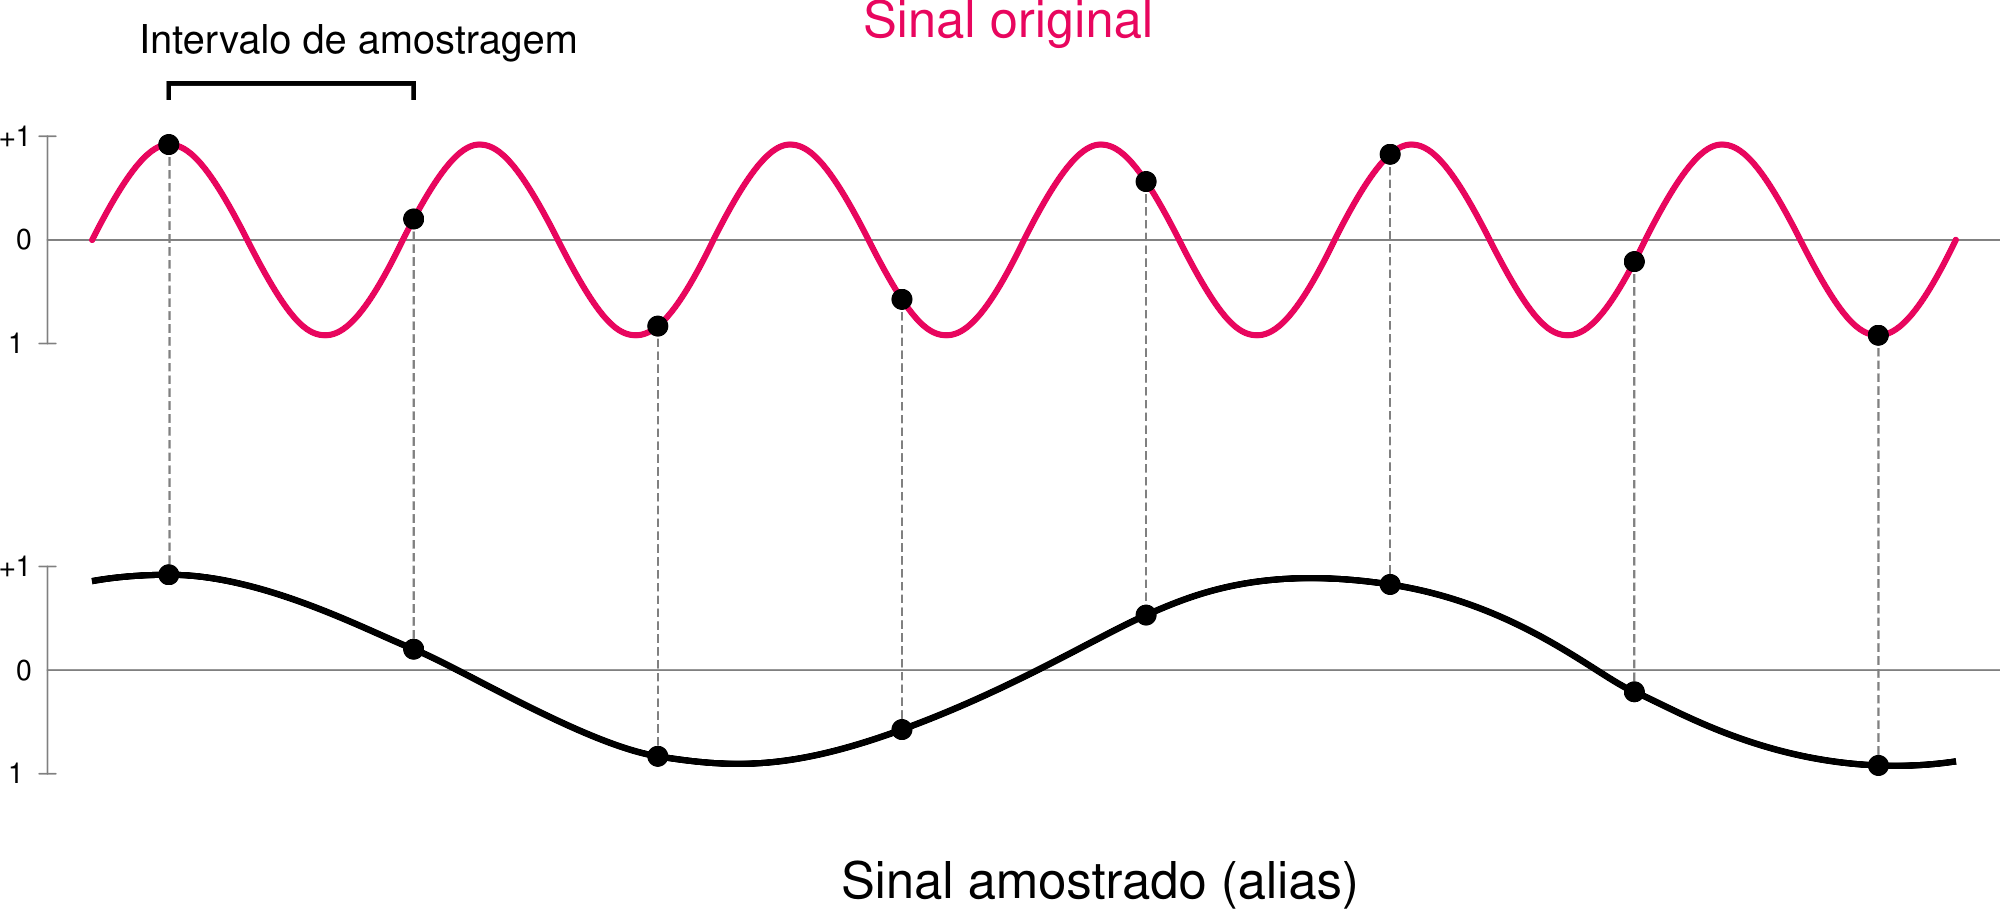
\includegraphics[width=0.7\linewidth]{Cap02/img/aliasing_wikimedia.png}
  \fonte{adaptado de \citeonline{krol_aliasing}, licença CC0.}
  \nota{sinal original em rosa; sinal percebido a partir das amostras em preto.}
\end{figure}

Para um analisador lógico, o requisito prático é ainda mais estrito que o
limite teórico. A reconstrução fiel de uma forma de onda digital, incluindo
a posição temporal das bordas, a largura de pulsos estreitos e \emph{glitches}, exige tipicamente uma taxa de amostragem de quatro a dez vezes a frequência
fundamental do sinal observado e, mais importante, exige que o intervalo entre
amostras seja constante: qualquer variação no período de amostragem se
traduz diretamente em erro na posição medida das bordas
\cite{smith1999,gis2021}.

\section{Determinismo temporal em sistemas embarcados}\label{sec:determinismo}

Em sistemas de aquisição, o termo determinismo designa a propriedade
de um evento de software ou hardware ocorrer em instantes previsíveis,
ciclo a ciclo. Três grandezas caracterizam o desvio desse ideal
\cite{lee2017,gis2021,alonso2024}:

\begin{itemize}
  \item \textbf{Latência}: o atraso entre um evento físico (por exemplo, uma borda de sinal) e a reação do sistema (o registro da amostra ou o início da captura); na Figura~\ref{fig:latencia-jitter-vazao}, corresponde ao deslocamento entre o evento esperado e a resposta real;
  \item \textbf{\emph{Jitter}}: a variação estatística dessa latência ou, no caso da amostragem periódica, a variação do intervalo entre amostras consecutivas em torno do período nominal; na Figura~\ref{fig:latencia-jitter-vazao}, é a diferença de latência de um ciclo para outro;
  \item \textbf{Vazão} (\emph{throughput}): a quantidade de dados que o sistema sustenta por unidade de tempo sem perdas; na Figura~\ref{fig:latencia-jitter-vazao}, é a taxa de amostras sustentada no intervalo observado.
\end{itemize}

\begin{figure}[H]
  \centering
  \caption{Latência, \emph{jitter} e vazão.}
  \label{fig:latencia-jitter-vazao}
  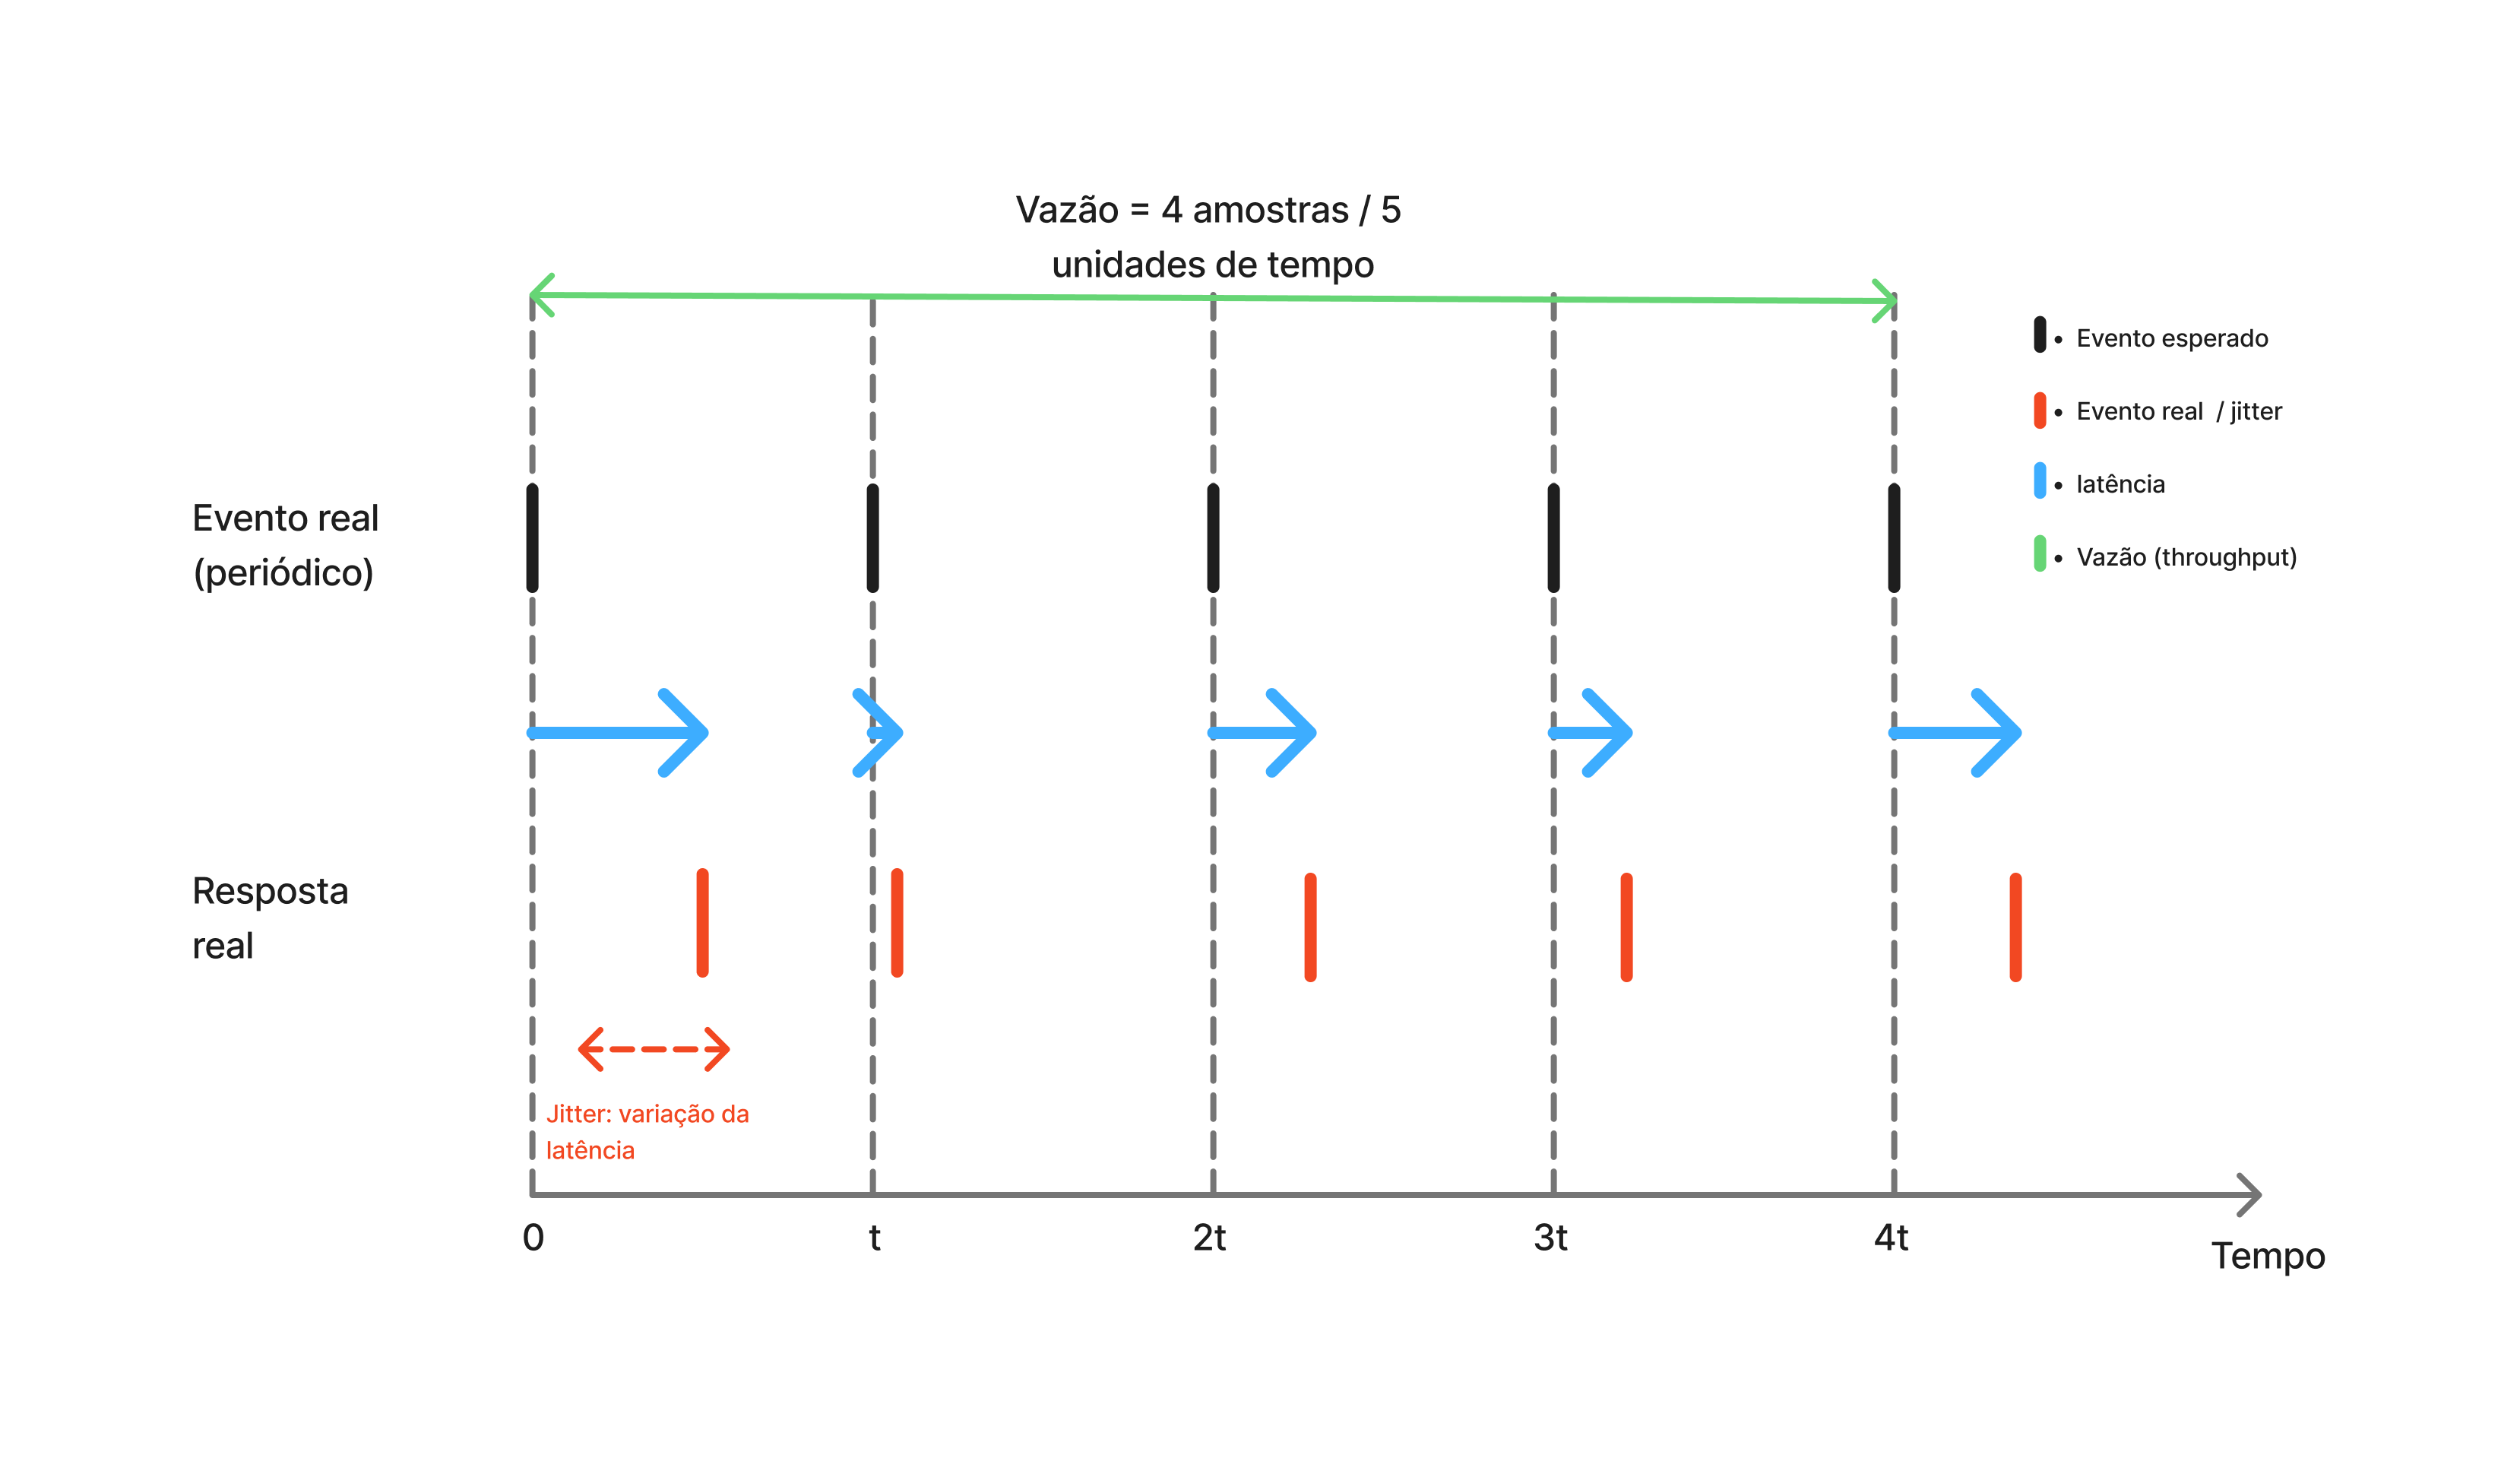
\includegraphics[width=0.85\linewidth]{Cap02/img/latencia_jitter_vazao.png}
  \fonte{Autoria própria.}
\end{figure}

Em um microcontrolador executando o padrão \ac{GPIO} com \ac{CPU}, captura de
sinais digitais por \emph{polling} ou interrupção, as causas vistas na Figura~\ref{fig:latencia-jitter-vazao}
tornam-se observáveis na Figura~\ref{fig:fontes-jitter-gpio-cpu}: diversas
fontes degradam o determinismo \cite{lee2017,ungurean2020,alonso2024}:

\begin{enumerate}
  \item \textbf{Latência de interrupção}: entre a ativação de uma \ac{IRQ} e a primeira instrução útil da \ac{ISR} decorre, já no melhor caso, da ordem de uma dezena de ciclos (tipicamente 12 no Cortex-M33, para salvamento de contexto, resolução de prioridade e busca do vetor), e esse número cresce e varia conforme a instrução em execução no momento e o estado do \emph{pipeline} \cite{arm2021};
  \item \textbf{Concorrência de interrupções}: \acp{ISR} de maior prioridade (por exemplo, da pilha \ac{USB}) atrasam a \ac{ISR} ou o laço de aquisição de forma imprevisível;
  \item \textbf{Troca de contexto (\acs{RTOS})}: em sistemas com escalonador, o \emph{tick} periódico e as trocas de tarefa consomem ciclos e adiam o atendimento de eventos; como o firmware de referência deste trabalho é \emph{bare-metal}, construído sobre o Raspberry Pi Pico \ac{SDK} e sem \ac{RTOS} (Seção~\ref{sec:baremetal-vs-rtos}), essa fonte específica não se aplica à implementação avaliada, mas é listada aqui por completude, já que caracteriza o padrão \ac{GPIO} com \ac{CPU} em geral;
  \item \textbf{Hierarquia de memória}: em chips que executam código diretamente da flash externa, em modo de \ac{XIP}, uma falha de cache impõe esperas de dezenas de ciclos no meio de um laço que se pretendia de tempo constante;
  \item \textbf{Arbitragem de barramento}: acessos simultâneos de \ac{CPU}, \ac{DMA} e periféricos à mesma \ac{SRAM} podem inserir ciclos de espera.
\end{enumerate}


A Figura~\ref{fig:fontes-jitter-gpio-cpu} resume essa cadeia de fontes, do evento físico
ao registro final da amostra. Para a amostragem periódica, o efeito agregado dessas fontes é o \emph{jitter}
de amostragem, que corrompe a base de tempo da aquisição: uma amostra tomada
tarde demais desloca a borda medida, e o erro não é recuperável por
pós-processamento. É por essa razão que plataformas de aquisição de alta
velocidade tradicionalmente recorrem a hardware dedicado, \acp{ASIC} ou \acp{FPGA}, em
que a amostragem é síncrona a um clock físico e imune ao estado do software
\cite{dai2017,gis2021}. O custo dessas soluções, entretanto, é justamente a
barreira que a instrumentação baseada em microcontrolador busca contornar,
conforme demonstram \citeonline{hercog2014} e \citeonline{romanov2021}.

\begin{figure}[htbp]
  \centering
  \caption{Fontes de não determinismo no padrão GPIO+CPU.}
  \label{fig:fontes-jitter-gpio-cpu}
  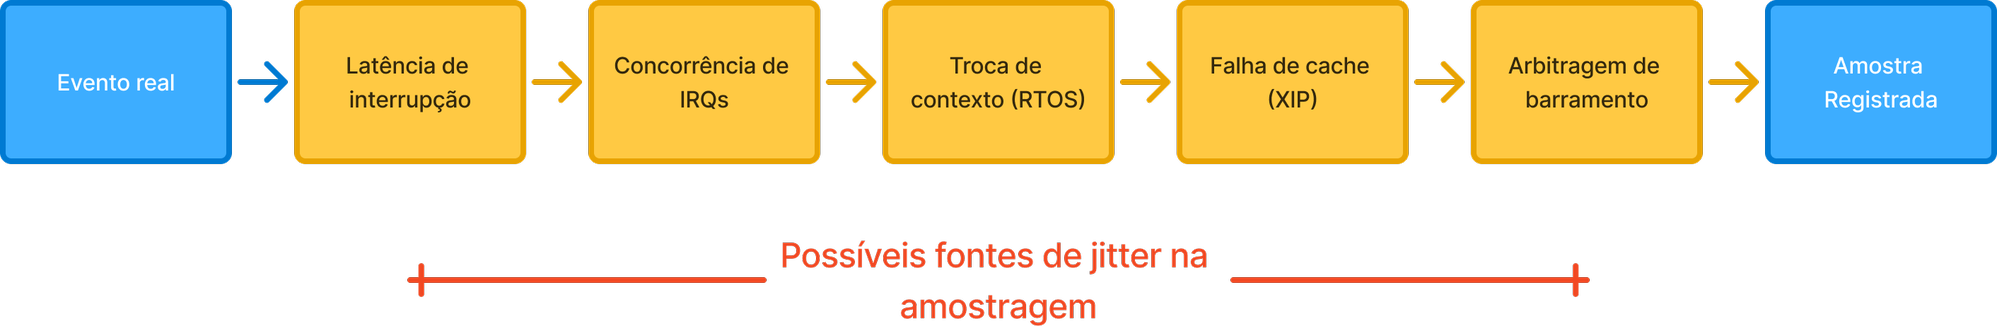
\includegraphics[width=0.9\linewidth]{Cap02/img/fontes_jitter_gpio_cpu.png}
  \fonte{Autoria própria.}
\end{figure}

\section{Aquisição por software}

\subsection{Aquisição com \emph{polling}}\label{sec:polling}

A abordagem mais direta para capturar sinais digitais em um \ac{MCU} é ler
periodicamente o registrador de entrada dos \acp{GPIO} com a própria \ac{CPU}, técnica
conhecida como \emph{polling} \cite{patterson2017}. Um laço mínimo de
amostragem executa, a cada iteração: a leitura do registrador de entrada, o
armazenamento do valor em um buffer, o avanço do ponteiro e o desvio
condicional de volta ao início. A taxa de amostragem máxima é, portanto,
limitada por:

\begin{equation}\label{eq:fsmax}
  f_{s,\max} = \frac{f_{clk}}{C_{iter}}
\end{equation}

\noindent em que $f_{clk}$ é a frequência da \ac{CPU} e $C_{iter}$ o número de ciclos por iteração do laço. Mesmo em um laço cuidadosamente otimizado em C ou assembly, da ordem de 4 a 8 ciclos por iteração em um Cortex-M33 com buffer em \ac{SRAM}, um clock de \ac{CPU} de 150\,MHz limita a amostragem a poucas dezenas de mega-amostras por segundo \emph{no melhor caso}, e qualquer instrução adicional (verificação de parada, controle de taxa, empacotamento) reduz esse teto proporcionalmente \cite{patterson2017,rpi2024ds}.

Mais grave que o teto de vazão é a instabilidade do período: para
amostrar a uma taxa \emph{programável} (e não simplesmente ``o mais rápido
possível''), o laço precisa calibrar sua duração com instruções de espera ou
comparação contra um \emph{timer}, e cada evento assíncrono (interrupção da
pilha \ac{USB}, falha de cache \ac{XIP}, acesso concorrente de \ac{DMA} à \ac{SRAM}) alonga
iterações individuais, produzindo \emph{jitter}. Desabilitar as interrupções
elimina parte do problema, mas impede o atendimento da comunicação com o \emph{host}
durante a captura, o que inviabiliza a captura contínua com transmissão
simultânea (\emph{streaming}).

\subsection{Aquisição com \emph{interrupção}}\label{sec:interrupt}

A alternativa por interrupção, configurar uma \ac{IRQ} de borda no \ac{GPIO} e
registrar amostras na \ac{ISR}, desloca o problema sem resolvê-lo: em frequências
altas, transições rápidas geram interrupções em cadência superior à capacidade
de atendimento da \ac{CPU}, sobrecarregando-a e causando perda de amostras e
corrupção de dados, fenômeno descrito na literatura de sistemas como
\emph{receive livelock}, em que a vazão útil colapsa a zero quando a taxa de
eventos excede a capacidade de atendimento da \ac{CPU}
\cite{mogul1997,regehr2005,souza2020}. Por isso, a aquisição por interrupção é
adequada apenas a sinais esparsos e lentos e não foi incluída na comparação
experimental deste trabalho, que adota o \emph{polling} como representante da
abordagem por software.

Uma mitigação relevante em \acp{MCU} de dois núcleos é \textbf{dedicar um núcleo
  inteiro ao laço de amostragem}, deixando o outro responsável pela comunicação.
Essa variante elimina a disputa direta entre amostragem e \ac{USB}, mas não elimina
o teto de vazão do laço nem as interferências de barramento e de memória e
ocupa integralmente um recurso computacional que, na arquitetura por hardware,
permanece livre. Essa variante é descrita na Seção~\ref{sec:firmware-b}, mas
não foi avaliada experimentalmente, ficando como trabalho futuro
(Seção~\ref{sec:trabalhos-futuros}).

\section{Aquisição por hardware: RP2350B}\label{sec:hardware}


\subsection{O microcontrolador RP2350}

O RP2350, da Raspberry Pi, é um microcontrolador de dois núcleos, ARM
Cortex-M33 ou RISC-V Hazard3, selecionáveis na inicialização, operando
tipicamente a 150\,MHz, com 520\,KB de \ac{SRAM} interna (512\,KB principais, distribuídos em oito
bancos, e dois bancos auxiliares de 4\,KB) e sem
memória flash interna: o código reside em uma flash \ac{QSPI} externa e é executado
via \ac{XIP} com cache \cite{rpi2024ds}. O chip dispõe de um
\ac{SIO}, que permite à \ac{CPU} ler o estado de todos os \acp{GPIO} em uma única
instrução, recurso central para a variante por software deste trabalho, além de
um conversor analógico-digital de 12 bits e dos subsistemas \ac{PIO} e \ac{DMA} descritos
a seguir. A variante RP2350B, utilizada na plataforma deste trabalho, expõe 48
\acp{GPIO} \cite{rpi2024ds}. A Figura~\ref{fig:rp2350-bus} mostra o
\emph{crossbar} \ac{AHB}5 que interliga esses recursos: os dois núcleos, o \ac{DMA} e os
periféricos (incluindo os três blocos \ac{PIO}) disputam as portas de \ac{SRAM}, \ac{XIP} e
\ac{APB}, e é justamente nesse ponto de disputa que se origina a arbitragem de
barramento citada como fonte de \emph{jitter} na Seção~\ref{sec:determinismo}.

\begin{figure}[htbp]
  \centering
  \caption{\emph{Crossbar} AHB5 do RP2350.}
  \label{fig:rp2350-bus}
  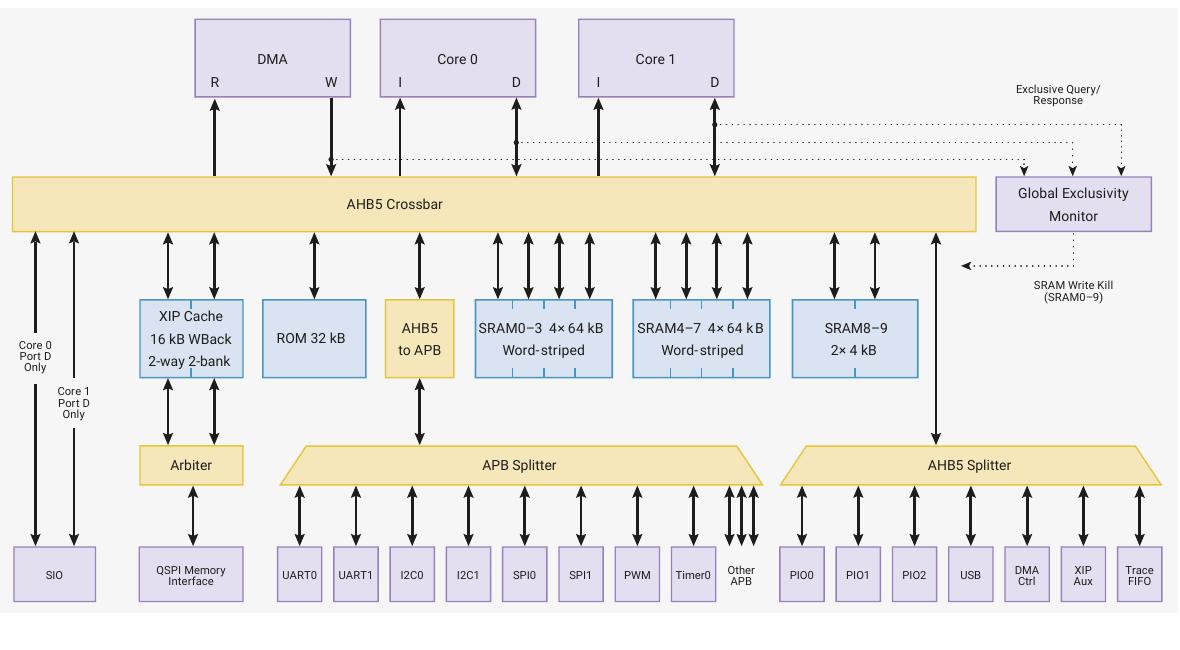
\includegraphics[width=0.7\linewidth]{Cap02/img/rp2350_bus_fabric.png}
  \fonte{\citeonline{rpi2024ds}.}
\end{figure}

\subsection{O subsistema PIO}\label{sec:pio}

O \ac{PIO} (\emph{Programmable Input/Output}) é o diferencial arquitetural da
família RP2 para aplicações de aquisição. Trata-se de blocos independentes
contendo, cada um, quatro \acp{SM} de hardware que executam um
conjunto de instruções próprio, minimalista e determinístico, em que cada
instrução executa em exatamente um ciclo do clock da máquina de estados
\cite{rpi2024ds}. O RP2350 integra três blocos \ac{PIO}, totalizando doze máquinas
de estados. A Figura~\ref{fig:pio-block} detalha a organização interna de um
desses blocos: as quatro máquinas de estado independentes compartilham a
memória de instruções e trocam dados com o barramento do sistema por meio de
\acp{FIFO} de hardware, sem intervenção da \ac{CPU}.

\begin{figure}[H]
  \centering
  \caption{Diagrama de blocos do PIO.}
  \label{fig:pio-block}
  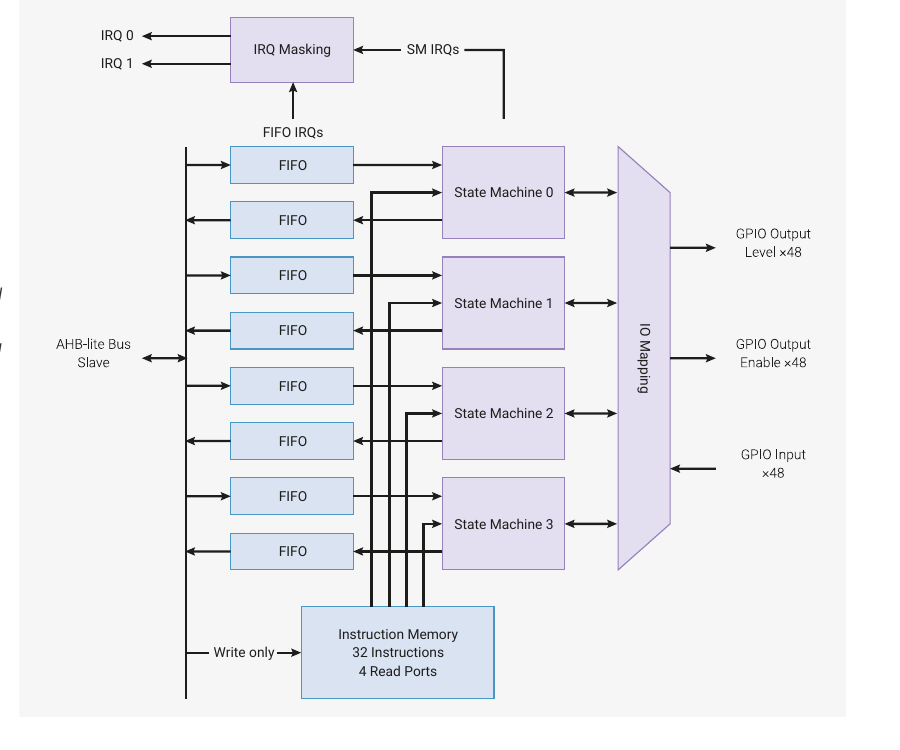
\includegraphics[width=0.75\linewidth]{Cap02/img/rp2350_pio_block_diagram.png}
  \fonte{\citeonline{rpi2024ds}.}
\end{figure}

Diferentemente de um laço de software na \ac{CPU}, uma máquina de estados \ac{PIO} pode
amostrar múltiplos pinos simultaneamente e empurrar os dados para um buffer
\ac{FIFO} de hardware, sem sofrer latência de interrupção, sobrecarga de troca de
contexto ou \emph{jitter} de execução, pois opera de forma totalmente
independente dos núcleos principais \cite{rpi2024ds,weber2025,mehr2025}. O
período de amostragem é definido por um divisor de clock fracionário próprio de
cada máquina de estados:

\begin{equation}\label{eq:clkdiv}
  \text{clkdiv} = \frac{f_{sys}}{f_{sample}}
\end{equation}

\noindent em que o divisor é representado em ponto fixo, com parte fracionária
de oito bits \cite{rpi2024ds}. Para divisores inteiros, o período de amostragem
é rigorosamente fixo em ciclos do clock do sistema. Para divisores
fracionários, a máquina de estados aproxima a taxa média alternando entre dois
períodos inteiros adjacentes, o que introduz um \emph{jitter} determinístico de
até um ciclo de $f_{sys}$, cerca de 6,7\,ns a 150\,MHz, no instante de
cada amostra \cite{rpi2024ds}. Esse limite é duas ordens de grandeza menor que
o período de amostragem nas taxas aqui investigadas e, ao contrário do laço de
\emph{polling} (Seção~\ref{sec:polling}), não depende do caminho de execução da
\ac{CPU} nem da latência de interrupção. Essa previsibilidade decorre do próprio
conjunto de instruções do \ac{PIO}, resumido a seguir.

\subsubsection{O conjunto de instruções do PIO}\label{sec:pio-isa}

O \ac{PIO} executa um conjunto reduzido de nove instruções, todas com duração fixa
de um ciclo de clock da máquina de estados (exceto quando programadas para
aguardar explicitamente), o que torna o tempo de execução de qualquer programa
previsível em tempo de compilação \cite{rpi2024ds}. Para a aquisição de
sinais digitais, duas instruções são centrais:

\begin{itemize}
  \item \texttt{in pins, N}: desloca o estado instantâneo de N pinos de
  entrada para o registrador de deslocamento e, quando este se enche, empurra
  automaticamente seu conteúdo para o \ac{FIFO} de recepção. Um programa de captura
  mínimo é essa única instrução em laço, produzindo uma amostra de N pinos por
  ciclo com comportamento \emph{cycle-accurate} que espelha o determinismo de
  um \ac{FPGA} a uma fração do custo \cite{rpi2024ds};
  \item \texttt{jmp pin}: desvia o fluxo do programa conforme o estado
  instantâneo de um \ac{GPIO} designado, sem consumir ciclos adicionais de
  amostragem, permitindo implementar disparo (\emph{trigger}) por borda ou por
  nível inteiramente em hardware \cite{rpi2024ds,starkey2024}.
\end{itemize}

\subsection{O subsistema DMA}

A captura contínua em alta taxa gera um fluxo de dados que rapidamente excede a
capacidade dos \acp{FIFO} internos do \ac{PIO} (quatro palavras por máquina de estados;
oito quando os \acp{FIFO} de transmissão e recepção são concatenados). Para evitar
transbordamento e perda de dados, emprega-se o controlador de \ac{DMA}: um
subsistema de hardware especializado em transferir dados entre periféricos e
memória sem intervenção da \ac{CPU} \cite{patterson2017,rpi2024ds}. No RP2350, cada
canal de \ac{DMA} pode ser ritmado pelo \ac{DREQ} do
periférico, de modo que a transferência avança automaticamente quando há dados
novos e estaciona quando o \ac{FIFO} esvazia. A Figura~\ref{fig:dma-architecture}
detalha essa arquitetura interna: gerentes de leitura e escrita independentes
movimentam dados entre memória e periféricos através de \acp{FIFO} de endereço e de
transferência, operando sobre o barramento do sistema sob supervisão apenas
dos registradores de controle e status.

\begin{figure}[H]
  \centering
  \caption{Arquitetura do controlador de DMA do RP2350.}
  \label{fig:dma-architecture}
  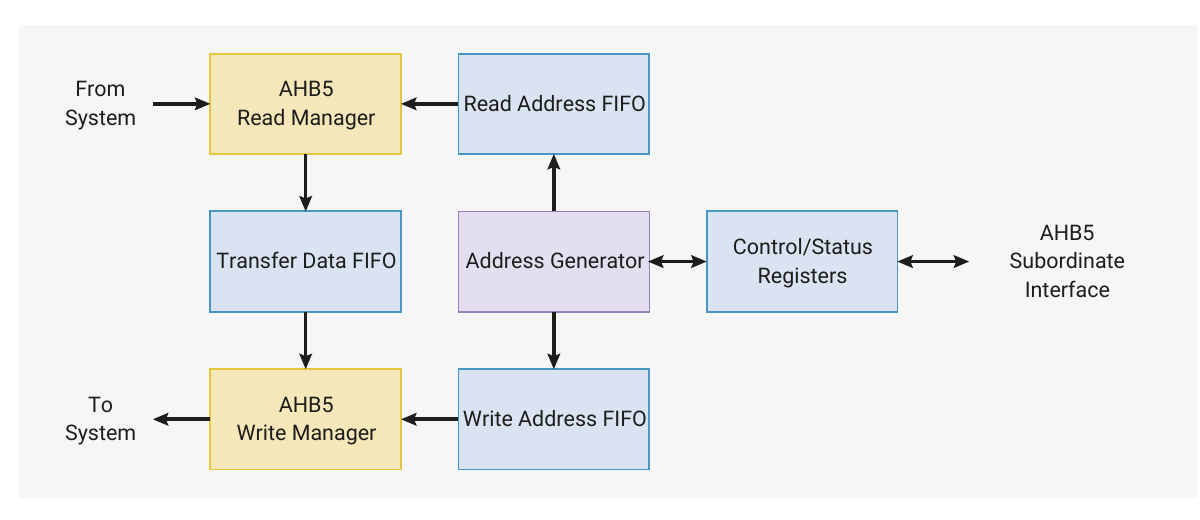
\includegraphics[width=0.85\linewidth]{Cap02/img/rp2350_dma_architecture.png}
  \fonte{\citeonline{rpi2024ds}.}
\end{figure}

Dois recursos são particularmente relevantes para aquisição contínua: o
\textbf{encadeamento de canais} e a operação em \textbf{\emph{ping-pong}}, em
que dois canais (ou dois blocos de descritores) se alternam entre duas metades
de um buffer enquanto o \ac{DMA} preenche uma metade, a \ac{CPU} (ou um segundo canal)
escoa a outra, com uma interrupção sinalizando cada troca de metade. Essa
técnica desacopla completamente a produção de amostras
(\ac{PIO}$\rightarrow$\ac{DMA}$\rightarrow$\ac{SRAM}) do consumo (\ac{SRAM}$\rightarrow$\ac{USB}),
permitindo \emph{streaming} sem lacunas \cite{rpi2024ds}.

Essa arquitetura reduz drasticamente a cadeia de fontes de \emph{jitter}
identificada para o padrão \ac{GPIO} com \ac{CPU} (Figura~\ref{fig:fontes-jitter-gpio-cpu}).
Como ilustra a Figura~\ref{fig:fontes-jitter-pio-dma}, o trecho crítico,
máquina de estados do \ac{PIO} $\rightarrow$ \ac{FIFO} de hardware $\rightarrow$
transferência via \ac{DMA} para a \ac{SRAM}, é inteiramente síncrono ao clock da
máquina de estados e ocorre sem intervenção da \ac{CPU}, portanto livre das fontes
de \emph{jitter} de software. O efeito de um
eventual atraso nesse trecho também muda de natureza: como a amostra já foi
capturada pelo \ac{PIO} no instante correto, um atraso na troca de \emph{buffer}
não desloca o instante de nenhuma amostra, e o risco passa a ser
\emph{overflow} da \ac{FIFO} (perda de amostras), não \emph{jitter} de
temporização.

\begin{figure}[H]
  \centering
  \caption{Fontes de não determinismo no padrão PIO+DMA.}
  \label{fig:fontes-jitter-pio-dma}
  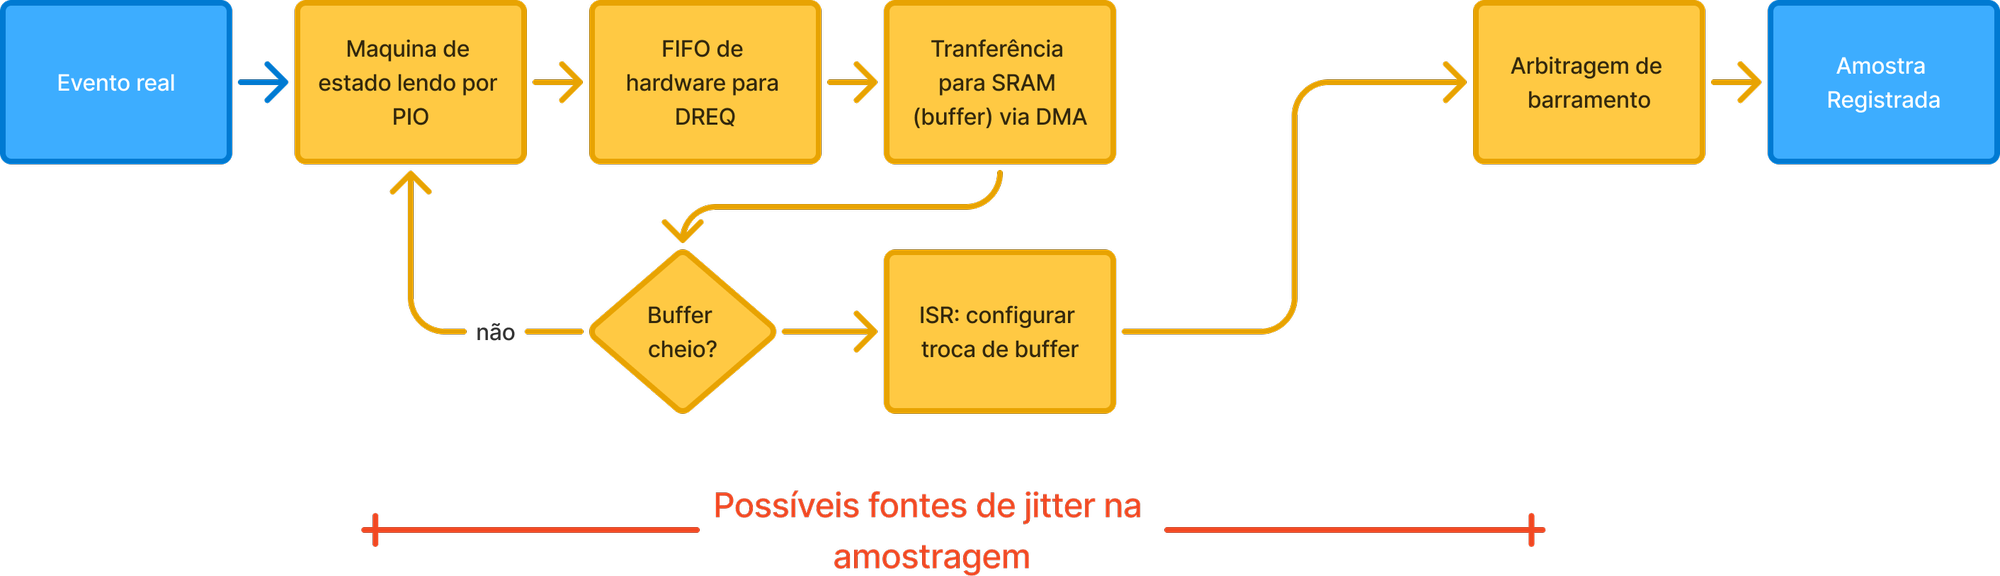
\includegraphics[width=0.95\linewidth]{Cap02/img/fontes_jitter_pio_dma.png}
  \fonte{Autoria própria.}
\end{figure}

A delegação da movimentação de dados ao \ac{DMA} é uma estratégia bastante conhecida
para maximizar a eficiência de sistemas embarcados com recursos restritos,
já que libera a \ac{CPU} de copiar cada dado entre periférico e memória
\cite{rpi2024ds}.

\subsection{Codificação (RLE)}

Depois que o \ac{DMA} deposita as amostras na \ac{SRAM}, a \ac{CPU} volta a entrar no
caminho de dados, mas fora do trecho crítico de captura: sua tarefa é
comprimir o \emph{buffer} por \acf{RLE} antes do envio via \ac{USB}, reduzindo a banda exigida
quando as linhas permanecem estáveis por várias amostras consecutivas. Em
vez de transmitir cada amostra, o \ac{RLE} transmite o valor e o número de
repetições consecutivas desse valor: uma linha estável por milhares de
amostras ocupa poucos \emph{bytes}. O ganho, porém, depende do sinal: um
sinal com transições a quase toda amostra praticamente não se compacta, de
modo que a banda exigida do \ac{USB} passa a depender do padrão capturado, efeito
que condiciona o desenho experimental (Seção~\ref{sec:bancada}). O formato
exato dos pares valor--repetição é definido pelo protocolo sigrok-pico
(Seção~\ref{sec:sigrok-pico}) e resumido na Seção~\ref{sec:firmware-a}.

\section{\emph{Bare-metal} \emph{versus} RTOS}\label{sec:baremetal-vs-rtos}

Um \acf{RTOS} introduz um escalonador cujo
\emph{tick} periódico realiza trocas de contexto entre tarefas, atribuindo
fatias de tempo e prioridades a cada uma delas. Esse mecanismo resolve um
problema de concorrência entre tarefas de propósito geral, mas não elimina o
não determinismo inerente ao restante do sistema: a latência de
escalonamento soma-se, e não substitui, as demais fontes de \emph{jitter}
discutidas na Seção~\ref{sec:determinismo} (latência de interrupção,
hierarquia de memória, arbitragem de barramento). Para uma tarefa em que a
temporização deve ser exata em ciclos e livre de \emph{jitter}, como a
amostragem de um analisador lógico, a sincronização de software oferecida por
um \ac{RTOS} não traz benefício sempre que a temporização crítica puder ser
garantida diretamente pelo hardware, e não pelo software
\cite{ungurean2020,hui2023}.

\section{O ecossistema Sigrok/PulseView e o protocolo sigrok-pico}\label{sec:sigrok-pico}

O Sigrok é uma suíte de software livre, portável e multiplataforma para
aquisição e análise de sinais, que abstrai dezenas de instrumentos por meio da
biblioteca \texttt{libsigrok}; o PulseView é seu \emph{front-end} gráfico, com
biblioteca de mais de duzentos decodificadores de protocolo: \ac{I2C}, \ac{SPI}, \ac{UART},
\ac{CAN}, RS-232, RS-485, entre outros, aplicáveis diretamente sobre os dados
capturados \cite{sigrok2026}. A Figura~\ref{fig:pulseview} mostra essa
decodificação em funcionamento: a faixa superior exibe um decodificador de
protocolo sobrepondo os bytes reconhecidos às formas de onda digitais brutas
exibidas logo abaixo.

\begin{figure}[htbp]
  \centering
  \caption{Captura decodificada no PulseView.}
  \label{fig:pulseview}
  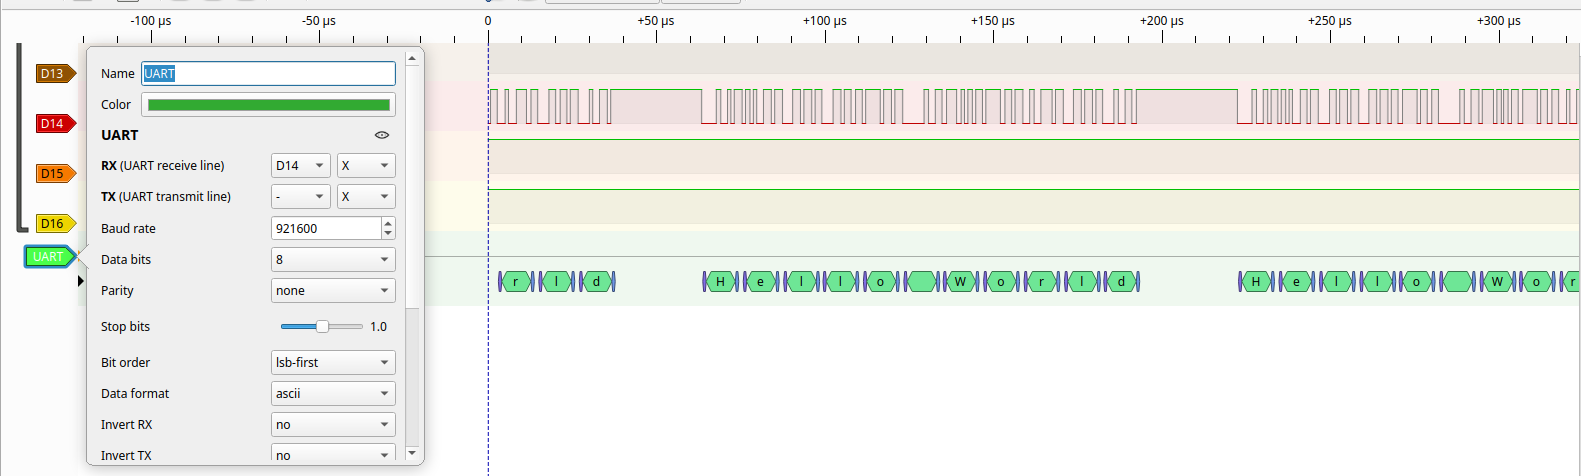
\includegraphics[width=0.95\linewidth]{Cap02/img/pulseview_screenshot.png}
  \fonte{adaptado de \citeonline{sigrok2026} (licença GNU GPL).}
\end{figure}

A adoção desse ecossistema como interface de
\emph{host} elimina os custos de licenciamento associados a softwares proprietários de
análise e transfere ao \emph{host} todo o processamento pesado (decodificação,
medição, exportação), exigindo do firmware apenas a conformidade com a
especificação do protocolo serial \textbf{sigrok-pico} \cite{picocoder2023}:
um protocolo textual simples sobre \ac{USB} \ac{CDC} explicitado no Quadro~\ref{qua:comandos}.

\section{Trabalhos relacionados}

O uso de microcontroladores da família RP2 como analisadores lógicos de baixo
custo tem precedentes na comunidade de software livre. O projeto
\textbf{sigrok-pico} \cite{picocoder2023}, origem do protocolo adotado,
implementa captura de até 21 canais digitais via \ac{PIO} com transferência por \ac{DMA}
no RP2040, com \emph{fork} posterior para o RP2350, e outros projetos
comunitários seguem a mesma linha. Esses projetos demonstram a viabilidade
da abordagem do \ac{PIO} associado ao \ac{DMA}, mas nenhum deles quantifica o ganho
sobre a alternativa por software: a escolha pelo \ac{PIO} é assumida como
evidente e não é medida.

Na literatura acadêmica, os trabalhos consultados cobrem partes da questão,
mas não a comparação em si. \citeonline{hercog2014} e \citeonline{romanov2021}
mostram que instrumentação de aquisição e análise lógica baseada em
microcontrolador é viável e reprodutível, sem contrapor arquiteturas de
captura. \citeonline{gis2021} e \citeonline{ungurean2020} caracterizam
experimentalmente o \emph{jitter} e o não determinismo da execução em
microcontroladores, fornecendo o arcabouço para as fontes discutidas na
Seção~\ref{sec:determinismo}, mas não em um instrumento de aquisição.
\citeonline{regehr2005} e \citeonline{mogul1997} descrevem o mecanismo pelo qual
sistemas dirigidos a interrupção saturam sob alta taxa de eventos
(Seção~\ref{sec:interrupt}). Por fim, \citeonline{weber2025}, \citeonline{starkey2024}
e \citeonline{mehr2025} empregam o \ac{PIO} e o \ac{DMA} do RP2040/RP2350 como periféricos
de temporização determinística em instrumentação científica, adotando o
hardware dedicado sem medi-lo contra a leitura por software. Nenhum desses
trabalhos mede, na mesma plataforma e sob as mesmas condições, taxa
sustentada, \emph{jitter}, perda de amostras e ocupação de \ac{CPU} das duas
arquiteturas, que é a comparação conduzida neste trabalho
(Capítulo~\ref{cap:metodologia}).
O Quadro~\ref{qua:trabalhos-relacionados} resume esse posicionamento.

\begin{quadro}[H]
  \centering
  \caption{Trabalhos relacionados.}
  \label{qua:trabalhos-relacionados}
  \small
  \begin{tabularx}{\linewidth}{|>{\raggedright\arraybackslash}p{3.1cm}|>{\raggedright\arraybackslash}X|>{\centering\arraybackslash}p{2.35cm}|>{\centering\arraybackslash}p{2.7cm}|}
    \hline
    \textbf{Trabalho} & \textbf{Contribuição} & \textbf{Usa PIO+DMA} & \textbf{Compara arquiteturas} \\ \hline
    \citeonline{picocoder2023} & Analisador lógico \ac{PIO}+\ac{DMA} no RP2040/RP2350; origem do protocolo sigrok-pico & \ding{51} & \ding{55} \\ \hline
    \citeonline{hercog2014}; \citeonline{romanov2021} & Instrumentação de aquisição e análise lógica baseada em microcontrolador & \ding{55} & \ding{55} \\ \hline
    \citeonline{gis2021}; \citeonline{ungurean2020} & Caracterização experimental do \emph{jitter} e do não determinismo em microcontroladores & \ding{55} & \ding{55} \\ \hline
    \citeonline{mogul1997}; \citeonline{regehr2005} & Saturação de sistemas dirigidos a interrupção (\emph{receive livelock}) & \ding{55} & \ding{55} \\ \hline
    \citeonline{weber2025}; \citeonline{starkey2024}; \citeonline{mehr2025} & \ac{PIO}/\ac{DMA} como temporização determinística em instrumentação científica & \ding{51} & \ding{55} \\ \hline
    \textbf{Este trabalho} & Taxa sustentada, \emph{jitter}, perda e ocupação de \ac{CPU} das duas arquiteturas, na mesma plataforma & \ding{51} & \ding{51} \\ \hline
  \end{tabularx}
  \fonte{Autoria própria.}
\end{quadro}

\cleardoublepage
% % % % % % % % % % % % % % % % % % % % % % % % % % %
\chapter{Metodologia}\label{cap:metodologia}

Este capítulo descreve como a comparação entre as arquiteturas de aquisição é
conduzida experimentalmente. Apresenta-se primeiro a visão geral do método,
junto com a bancada experimental e o hardware utilizado
(Seção~\ref{sec:bancada}), seguidos da implementação de cada firmware
(Seções~\ref{sec:firmware-a} e~\ref{sec:firmware-b}), das métricas e
procedimentos adotados em cada experimento (Seção~\ref{sec:metricas}) e da
análise estatística (Seção~\ref{sec:analise-estatistica}).

\section{Visão geral do método}

Este trabalho conduz uma comparação experimental controlada entre duas
arquiteturas de firmware de aquisição executando sobre o mesmo hardware, o
mesmo protocolo de \emph{host} e as mesmas condições de teste. O foco central é a
análise comparativa entre as configurações, mudando apenas o mecanismo de
amostragem e transporte interno dos dados, permanecendo idênticos a placa, o
clock do sistema, a pilha \ac{USB} (TinyUSB), o protocolo sigrok-pico, a
codificação \ac{RLE}, o software do \emph{host} e os sinais de estímulo. Dessa forma, diferenças
observadas nas métricas podem ser atribuídas à arquitetura de aquisição,
excluindo possíveis variações externas. Duas diferenças decorrem da própria
arquitetura e são mantidas de propósito: o disparo, feito pelo \ac{PIO} em A
e por comparação em software em B, e o tamanho dos \emph{buffers} de
amostras, maior em B para reduzir suas pausas de amostragem
(Seção~\ref{sec:firmware-b}). O hardware é tomado como plataforma
fixa, e a variável investigada é exclusivamente a arquitetura de firmware.

São comparadas duas configurações de firmware:

\begin{itemize}
  \item \textbf{Firmware A}: aquisição por \ac{PIO} com transferência por \ac{DMA} (Seção~\ref{sec:firmware-a});
  \item \textbf{Firmware B}: aquisição por leitura dos \acp{GPIO} pela própria \ac{CPU}, por meio do bloco \ac{SIO} e das funções do Pico \ac{SDK} \cite{rpi2024sdk} (Seção~\ref{sec:firmware-b}).
\end{itemize}

\subsection{Delimitação de autoria e disponibilidade dos artefatos}\label{sec:autoria}

Os dois firmwares comparados neste trabalho foram escritos pelo autor, assim
como a extensão do protocolo para consulta da ocupação de \ac{CPU} (comando
\texttt{'o'}), a instrumentação pelo contador de ciclos \ac{DWT}, a bancada
automatizada de medição e os \emph{scripts} de análise estatística. São de
terceiros, e tomados como plataforma fixa, a placa de aquisição
\cite{nivuciis_msa}, o protocolo de comunicação com o \emph{host}, herdado do
projeto sigrok-pico \cite{picocoder2023}, e a pilha \ac{USB} TinyUSB,
distribuída com o Pico \ac{SDK} \cite{rpi2024sdk}. O Firmware A é tomado como
linha de base da comparação; o Firmware B foi implementado especificamente para
esta investigação, em \emph{branch} dedicado a partir do mesmo \emph{commit}
base.

Os dois firmwares, os programas da bancada, os \emph{scripts} de análise e os
dados brutos de todas as repetições estão publicamente disponíveis
\cite{dias2026artefatos}, de modo que as medições relatadas no
Capítulo~\ref{cap:resultados} possam ser auditadas e repetidas por terceiros
\cite{collberg2016}.

\subsection{Bancada experimental}\label{sec:bancada}

A bancada experimental segue as recomendações da literatura de avaliação de
desempenho de sistemas computacionais para controle de variáveis externas e
rastreabilidade dos resultados \cite{georges2007,hoefler2015}: instrumentos,
versões de software e procedimentos de coleta são fixados e registrados antes
da execução das medições, de modo que a variável independente observada seja
exclusivamente a arquitetura de firmware (Seção~\ref{sec:firmware-a}
e~\ref{sec:firmware-b}).

A Figura~\ref{fig:conjunto} mostra o diagrama e a montagem física da
bancada, cujos componentes são descritos a seguir.

\begin{figure}[htbp]
  \centering
  \caption{Bancada experimental.}
  \label{fig:conjunto}
  \subfloat[Diagrama de fluxo da bancada.\label{fig:img1}]{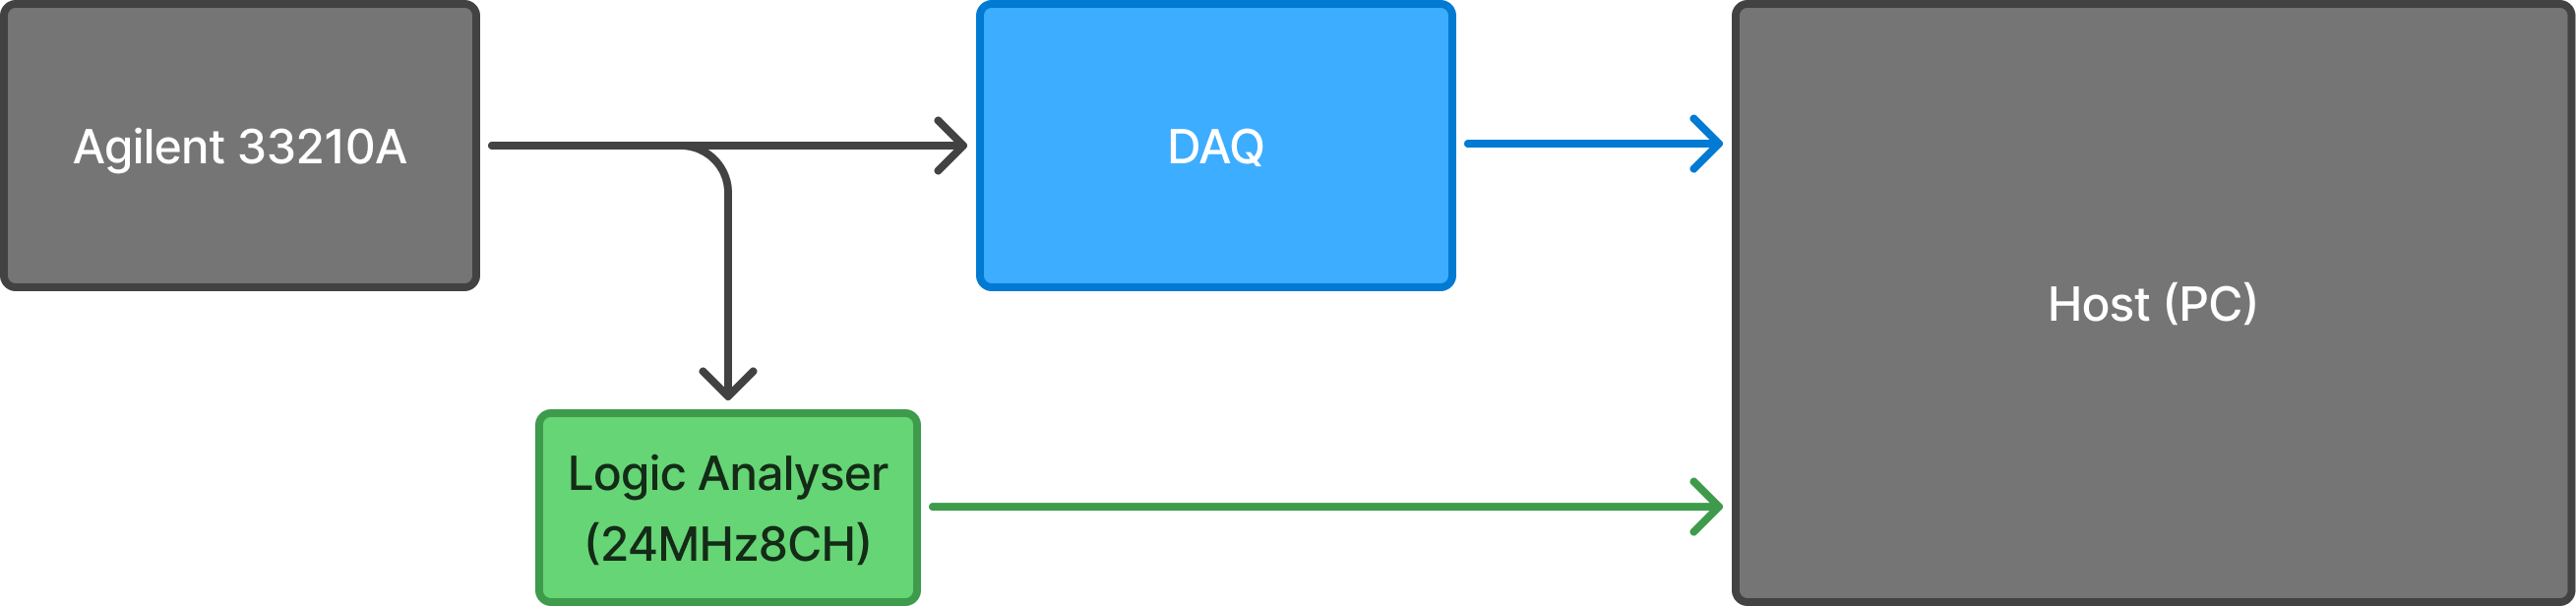
\includegraphics[width=0.45\linewidth]{Cap03/img/bancada_diagrama.png}}
  \hfill
  \subfloat[Montagem física: (A) gerador de funções Agilent 33210A; (B) DAQ baseado no RP2350B; (C) instrumento de referência.\label{fig:img2}]{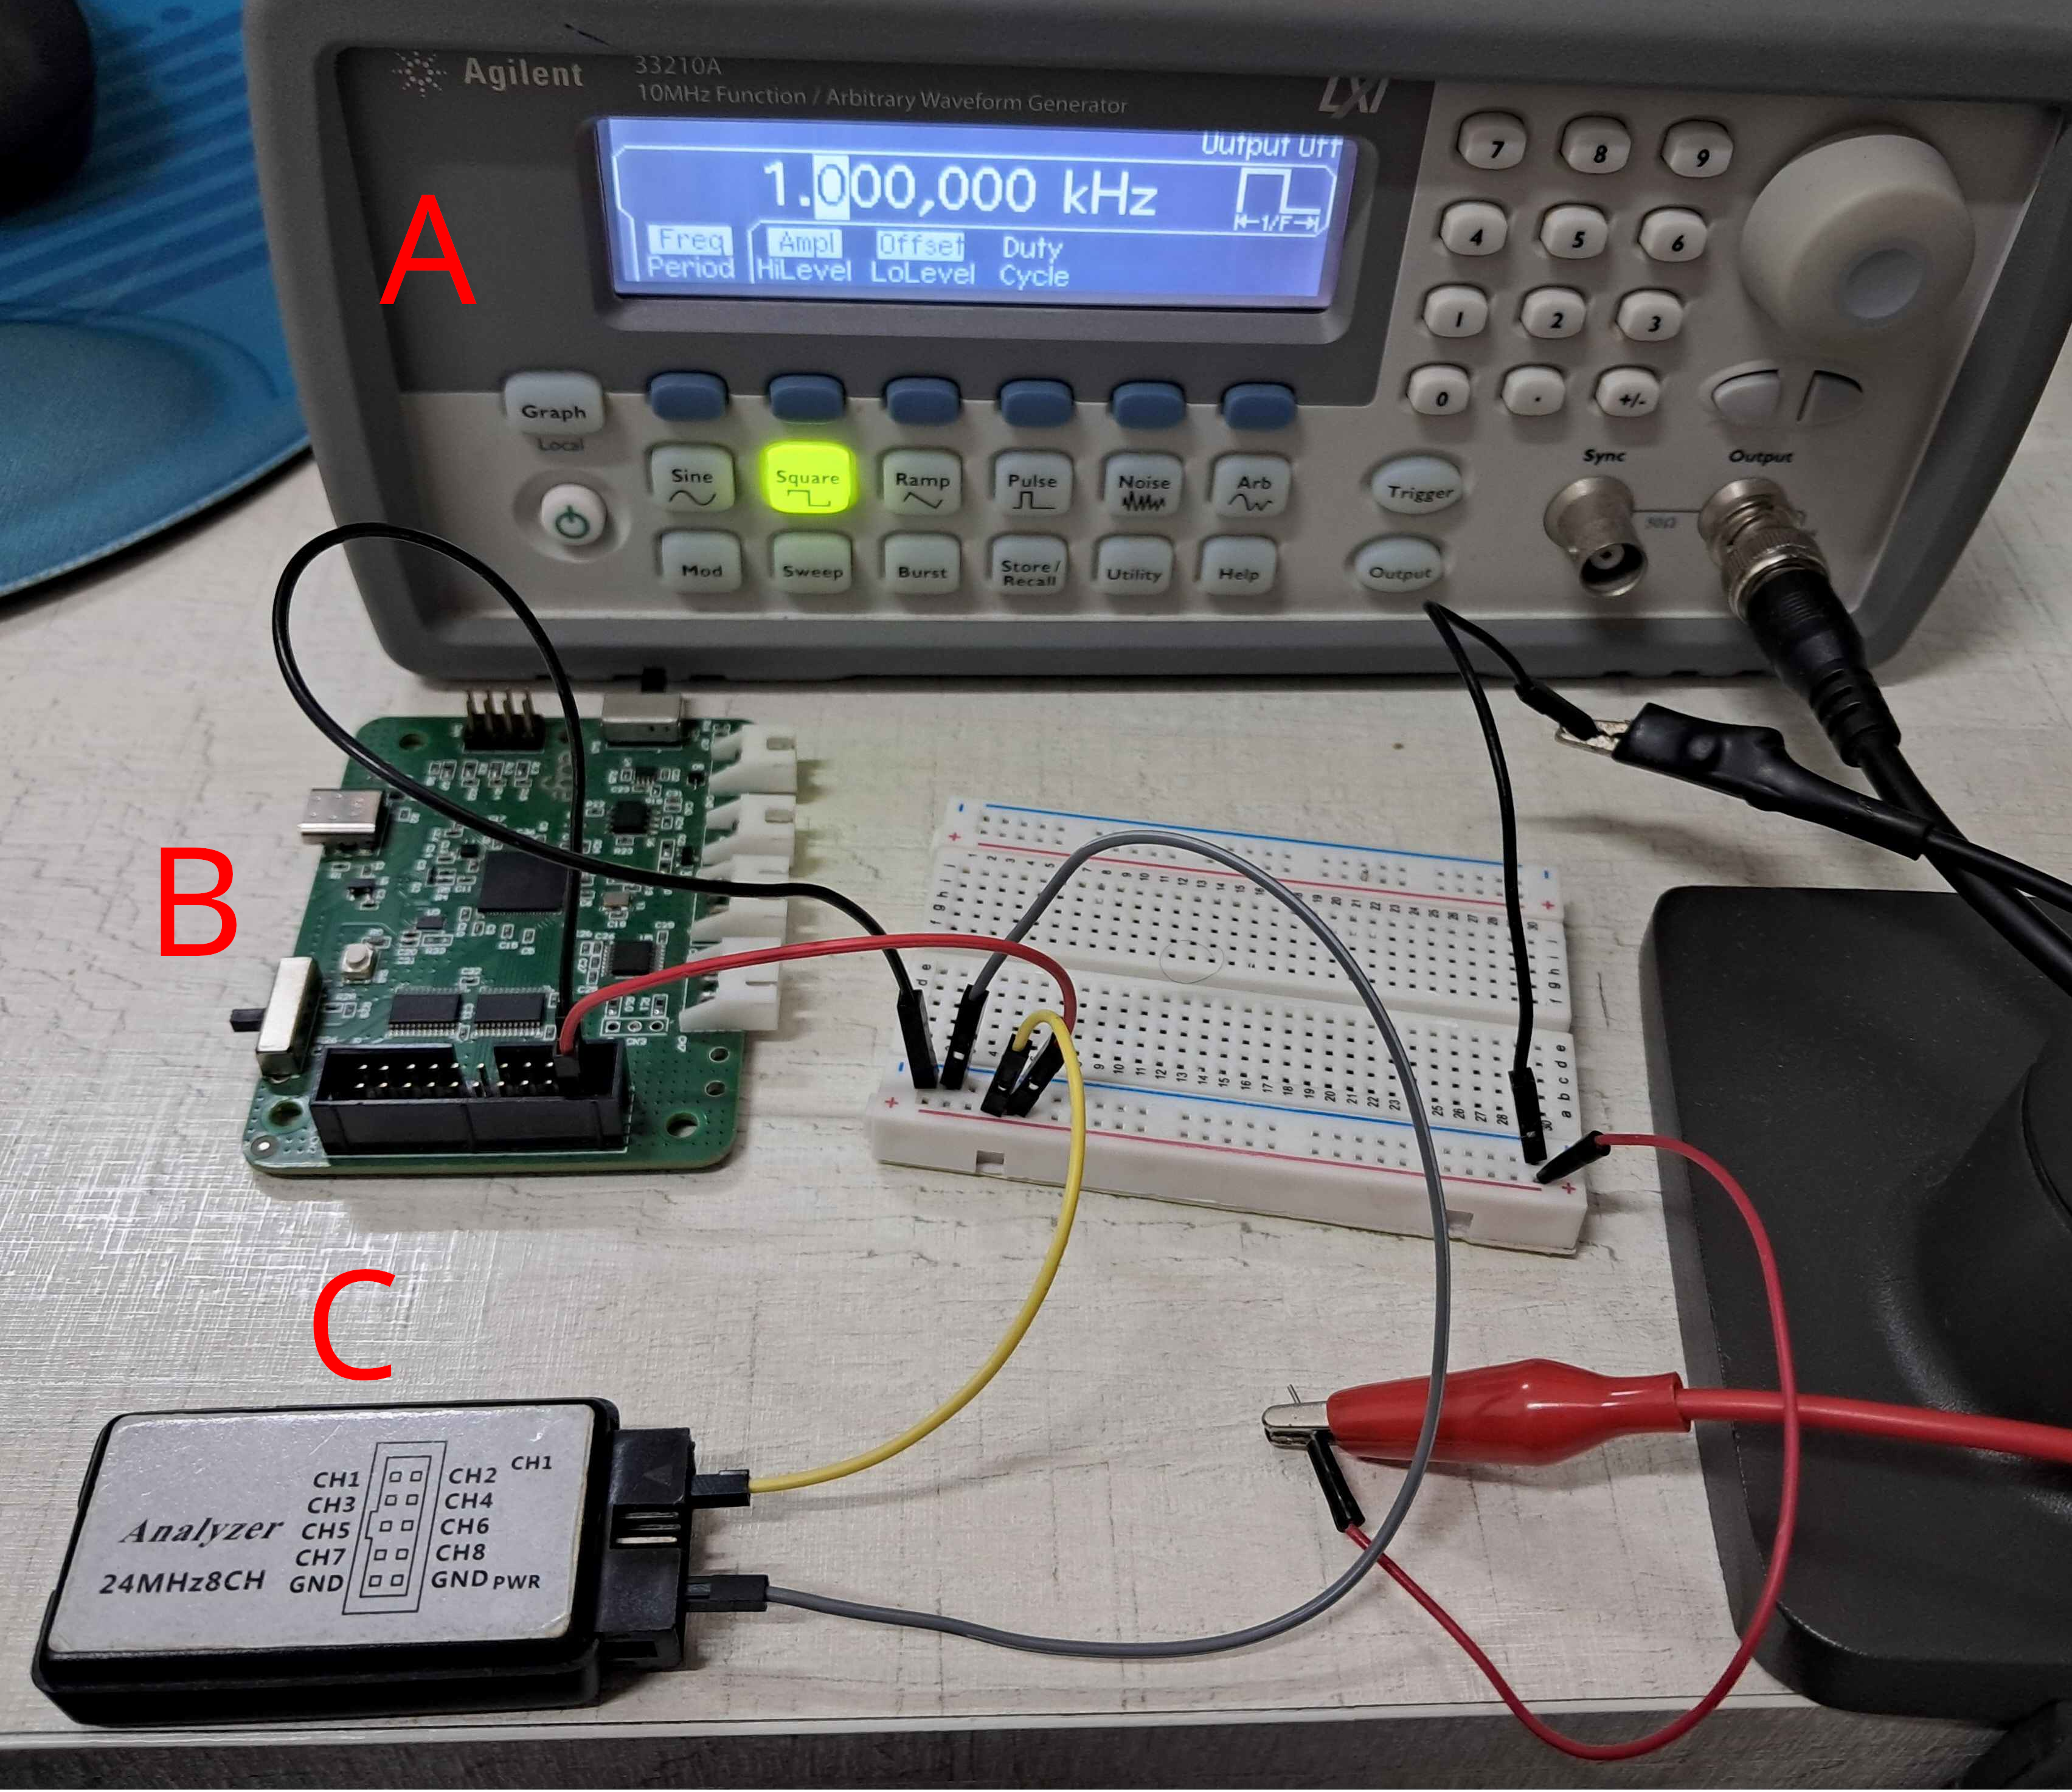
\includegraphics[width=0.45\linewidth]{Cap03/img/bancada_fisica.png}}
  \fonte{Autoria própria.}
\end{figure}

\subsubsection{Placa de aquisição e gerador de sinais}\label{sec:hardware-daq}

A plataforma é o \ac{DAQ}, centrado na RP2350B, com doze canais de
aquisição digital acessíveis por conector de cabo plano de 20 vias (com
tradução de nível para alvos de 1,8\,V a 5,0\,V) e interfaces passivas de
barramento industrial RS-485 e RS-232, não exercitadas nos experimentos, comunicando-se com o \emph{host} por \ac{USB} 2.0
Full Speed.

\begin{figure}[htbp]
  \centering
  \caption{Placa de aquisição (DAQ) baseada no RP2350B.}
  \label{fig:placa-daq}
  \subfloat[Face superior.]{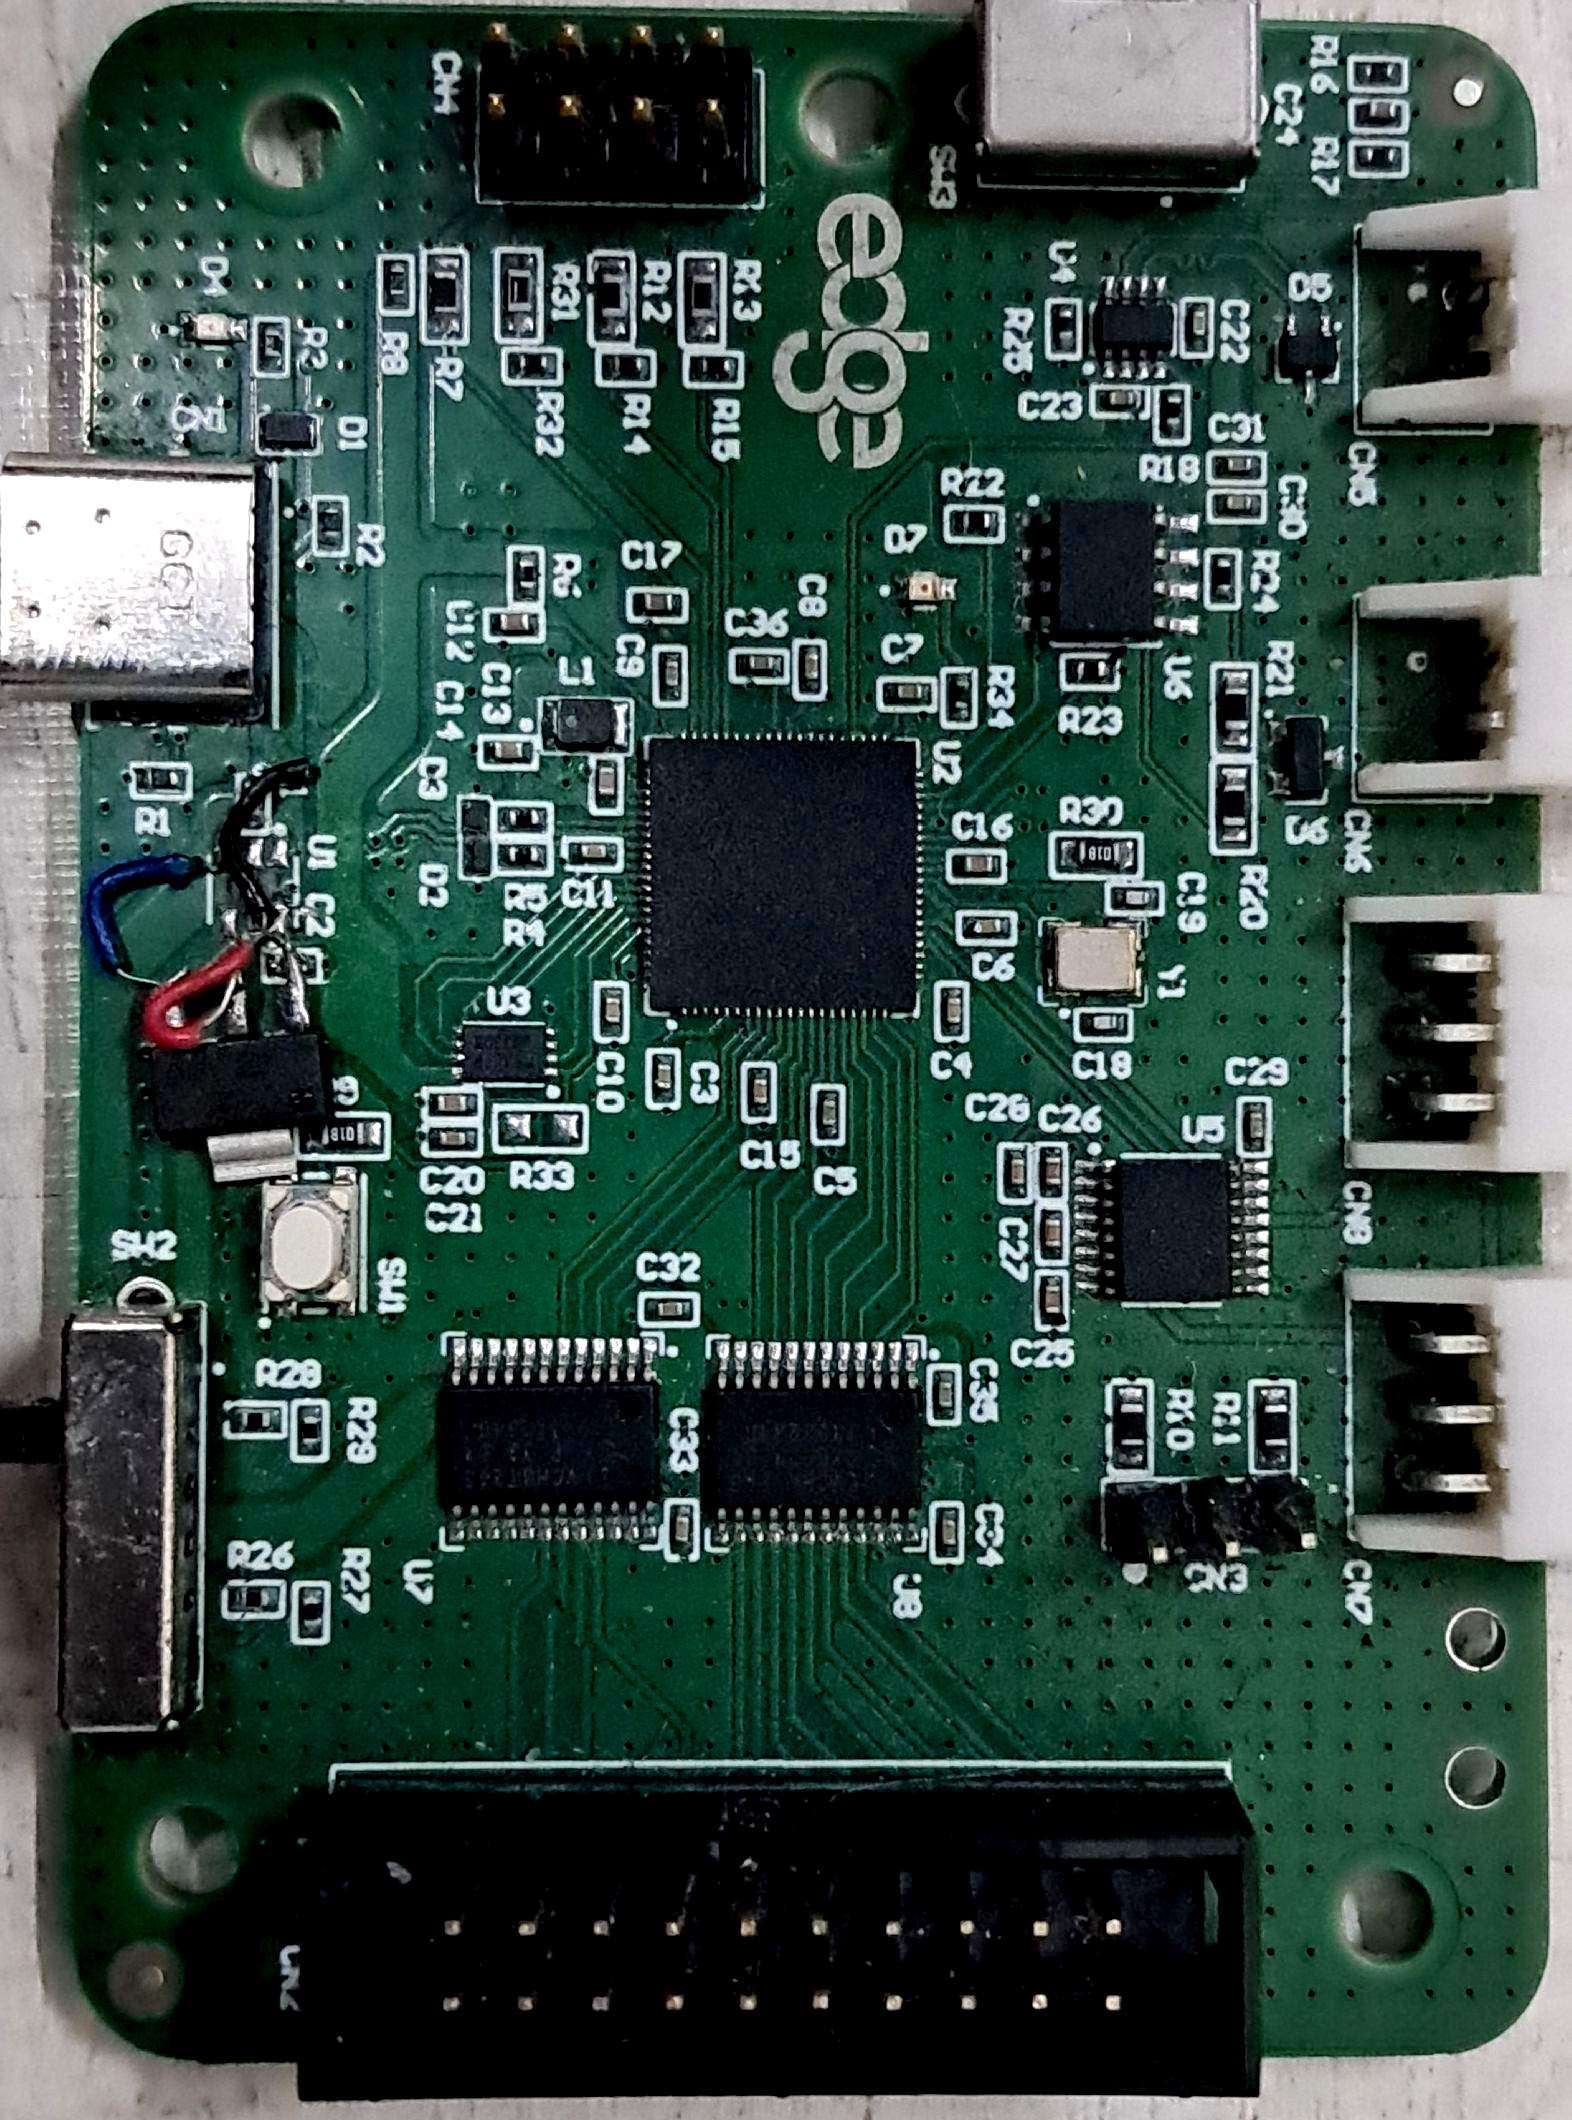
\includegraphics[width=0.45\linewidth]{Cap03/img/placa_daq_top.jpg}}
  \hfill
  \subfloat[Face inferior.]{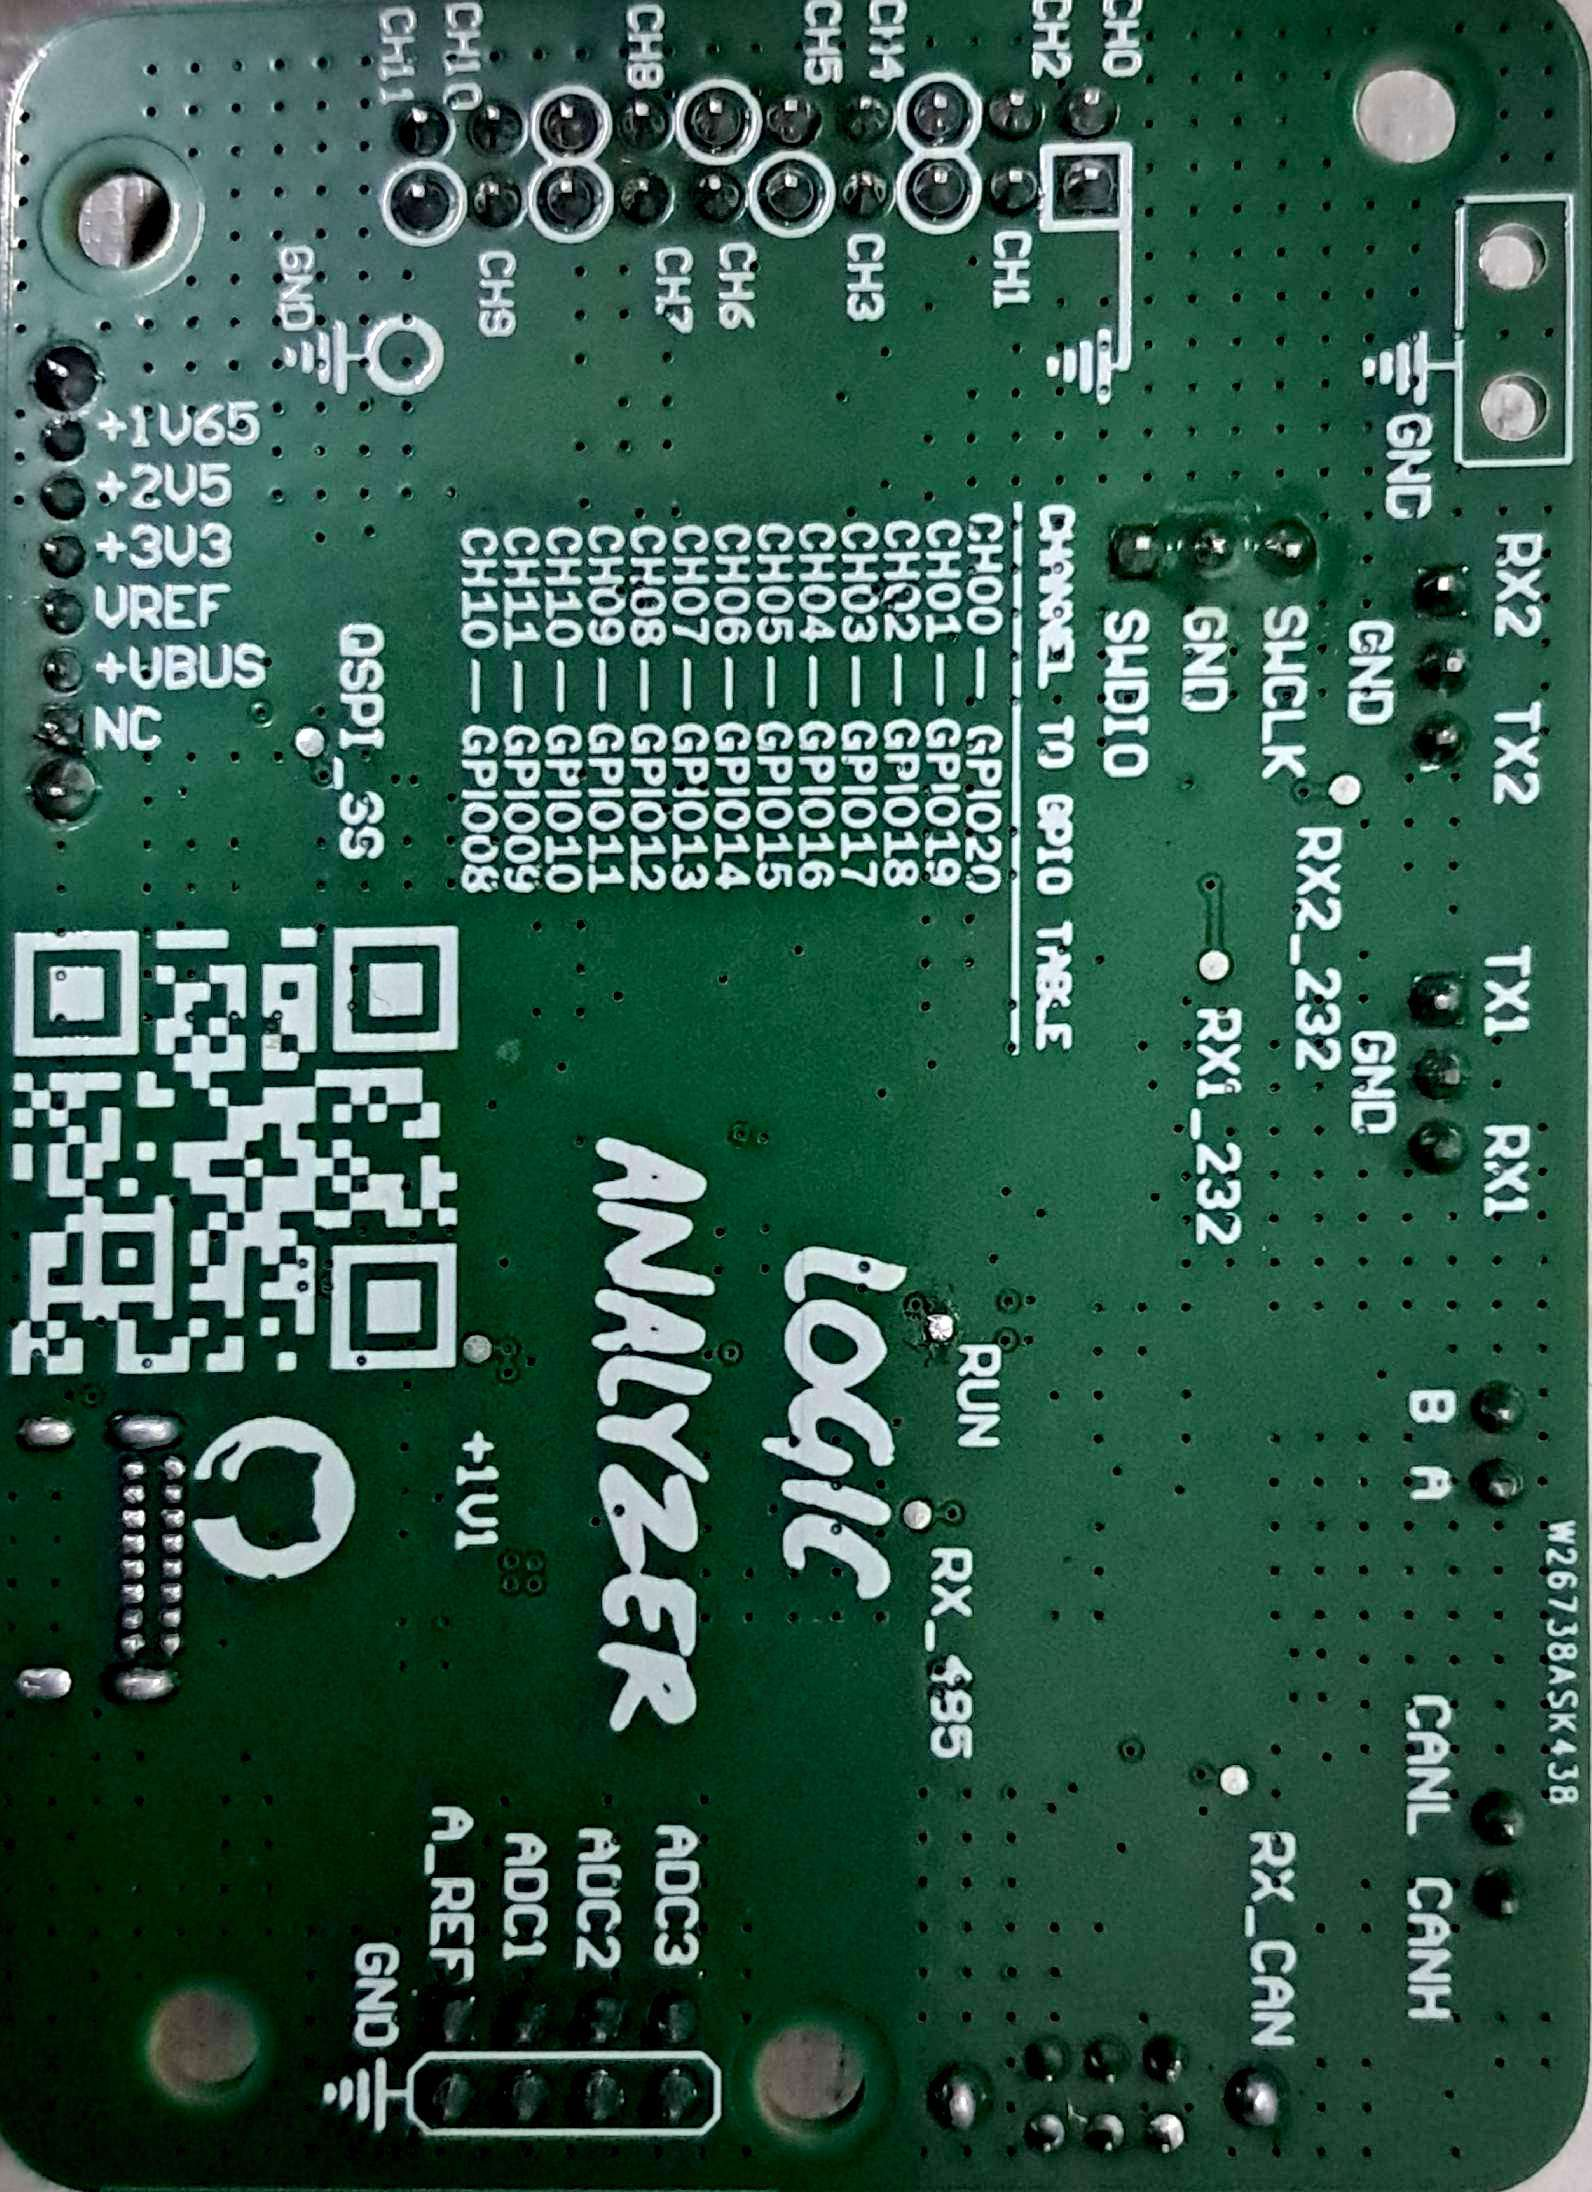
\includegraphics[width=0.45\linewidth]{Cap03/img/placa_daq_bottom.jpg}}
  \fonte{\citeonline{nivuciis_msa}.}
\end{figure}

Em altas velocidades, a integridade física do sinal impõe requisitos ao próprio
hardware de captura: trilhas devem ser tratadas como linhas de transmissão, com
impedância controlada e caminho de retorno de baixa indutância, sob pena de
reflexões e interferência eletromagnética corromperem o sinal antes mesmo da
amostragem \cite{bogatin2011,fan2010,morrison2007}. Esses aspectos foram
observados no projeto da placa utilizada neste trabalho
(Figura~\ref{fig:placa-daq}).

Um gerador de funções Agilent 33210A (até 10\,MHz) produz o sinal de entrada
de todos os ensaios.

\begin{figure}[htbp]
  \centering
  \caption{Gerador de funções Agilent 33210A.}
  \label{fig:gerador-agilent}
  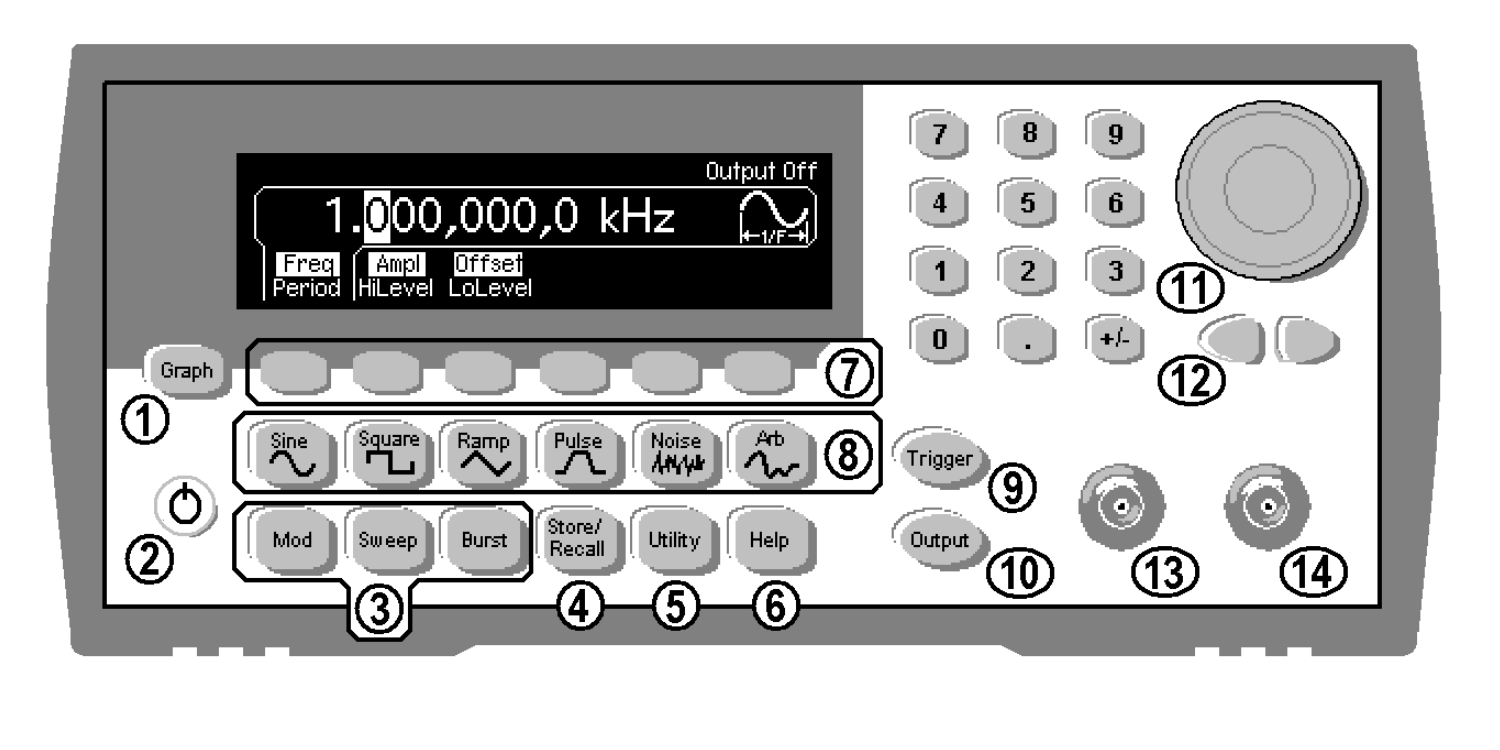
\includegraphics[width=0.5\linewidth]{Cap03/img/gerador_agilent_33210a.png}
  \fonte{adaptado de \citeonline{agilent2008}.}
\end{figure}

Como a banda do \ac{USB} 2.0 Full Speed (12\,Mbit/s) é ordens de grandeza inferior à
taxa de produção de amostras no limite da plataforma, o \ac{RLE}
(Seção~\ref{sec:sigrok-pico}) e o buffer em \ac{SRAM} são componentes essenciais do
caminho de dados em ambas as arquiteturas comparadas \cite{picocoder2023}.

\subsubsection{Instrumentos, \emph{host} e medição}\label{sec:bancada-instrumentos}

\begin{itemize}
  \item \textbf{Gerador de padrões:} o gerador de funções Agilent 33210A (Figura~\ref{fig:gerador-agilent}), configurado para produzir a onda quadrada de 100\,kHz usada em M1, M2 e M3 (em M4, 1\,MHz; ver Seção~\ref{sec:metricas}), aplicada em paralelo ao canal D3 do \ac{DAQ} e ao analisador lógico de referência. A frequência de 100\,kHz foi escolhida porque a compactação \ac{RLE} mantém o fluxo abaixo do teto do \ac{USB} Full-Speed em toda a faixa de taxas varrida; com 1\,MHz, o fluxo quase não se compacta e a medida passa a refletir o barramento, e não o amostrador.

  \item \textbf{Instrumento de referência:} analisador lógico \ac{USB} genérico de 8 canais e 24\,MHz, baseado no microcontrolador Cypress CY7C68013A (FX2LP) e compatível com o \emph{software} da Saleae (Figura~\ref{fig:instrumento-ref}), controlado pelo software Logic~2 (versão 2.4.44) por meio de sua \ac{API} de automação, usado como contador de bordas externo e para aferição da frequência do gerador. A cada repetição, o \emph{script} do \emph{host} arma o \ac{DAQ} e o analisador na mesma borda de subida e compara as duas capturas da mesma janela. Operado a 12\,MS/s, o analisador resolve o tempo em passos de 83,3\,ns, isto é, 120 amostras por período da onda de 100\,kHz, margem suficiente para a contagem de bordas e de períodos frente às taxas do \ac{DAQ} (até $\approx 5$\,MS/s). Sua base de tempo depende de um cristal sem calibração rastreável, o que limita a exatidão absoluta da frequência medida à tolerância desse cristal (tipicamente dezenas de ppm). A medição externa de tempos por um pino de \emph{debug} comutado pelo firmware não foi empregada (Seção~\ref{sec:trabalhos-futuros}); a métrica M4 é medida internamente por \ac{DWT} (item a seguir).

  \begin{figure}[htbp]
    \centering
    \caption{Analisador lógico de referência (FX2LP, 8 canais, 24\,MHz).}
    \label{fig:instrumento-ref}
    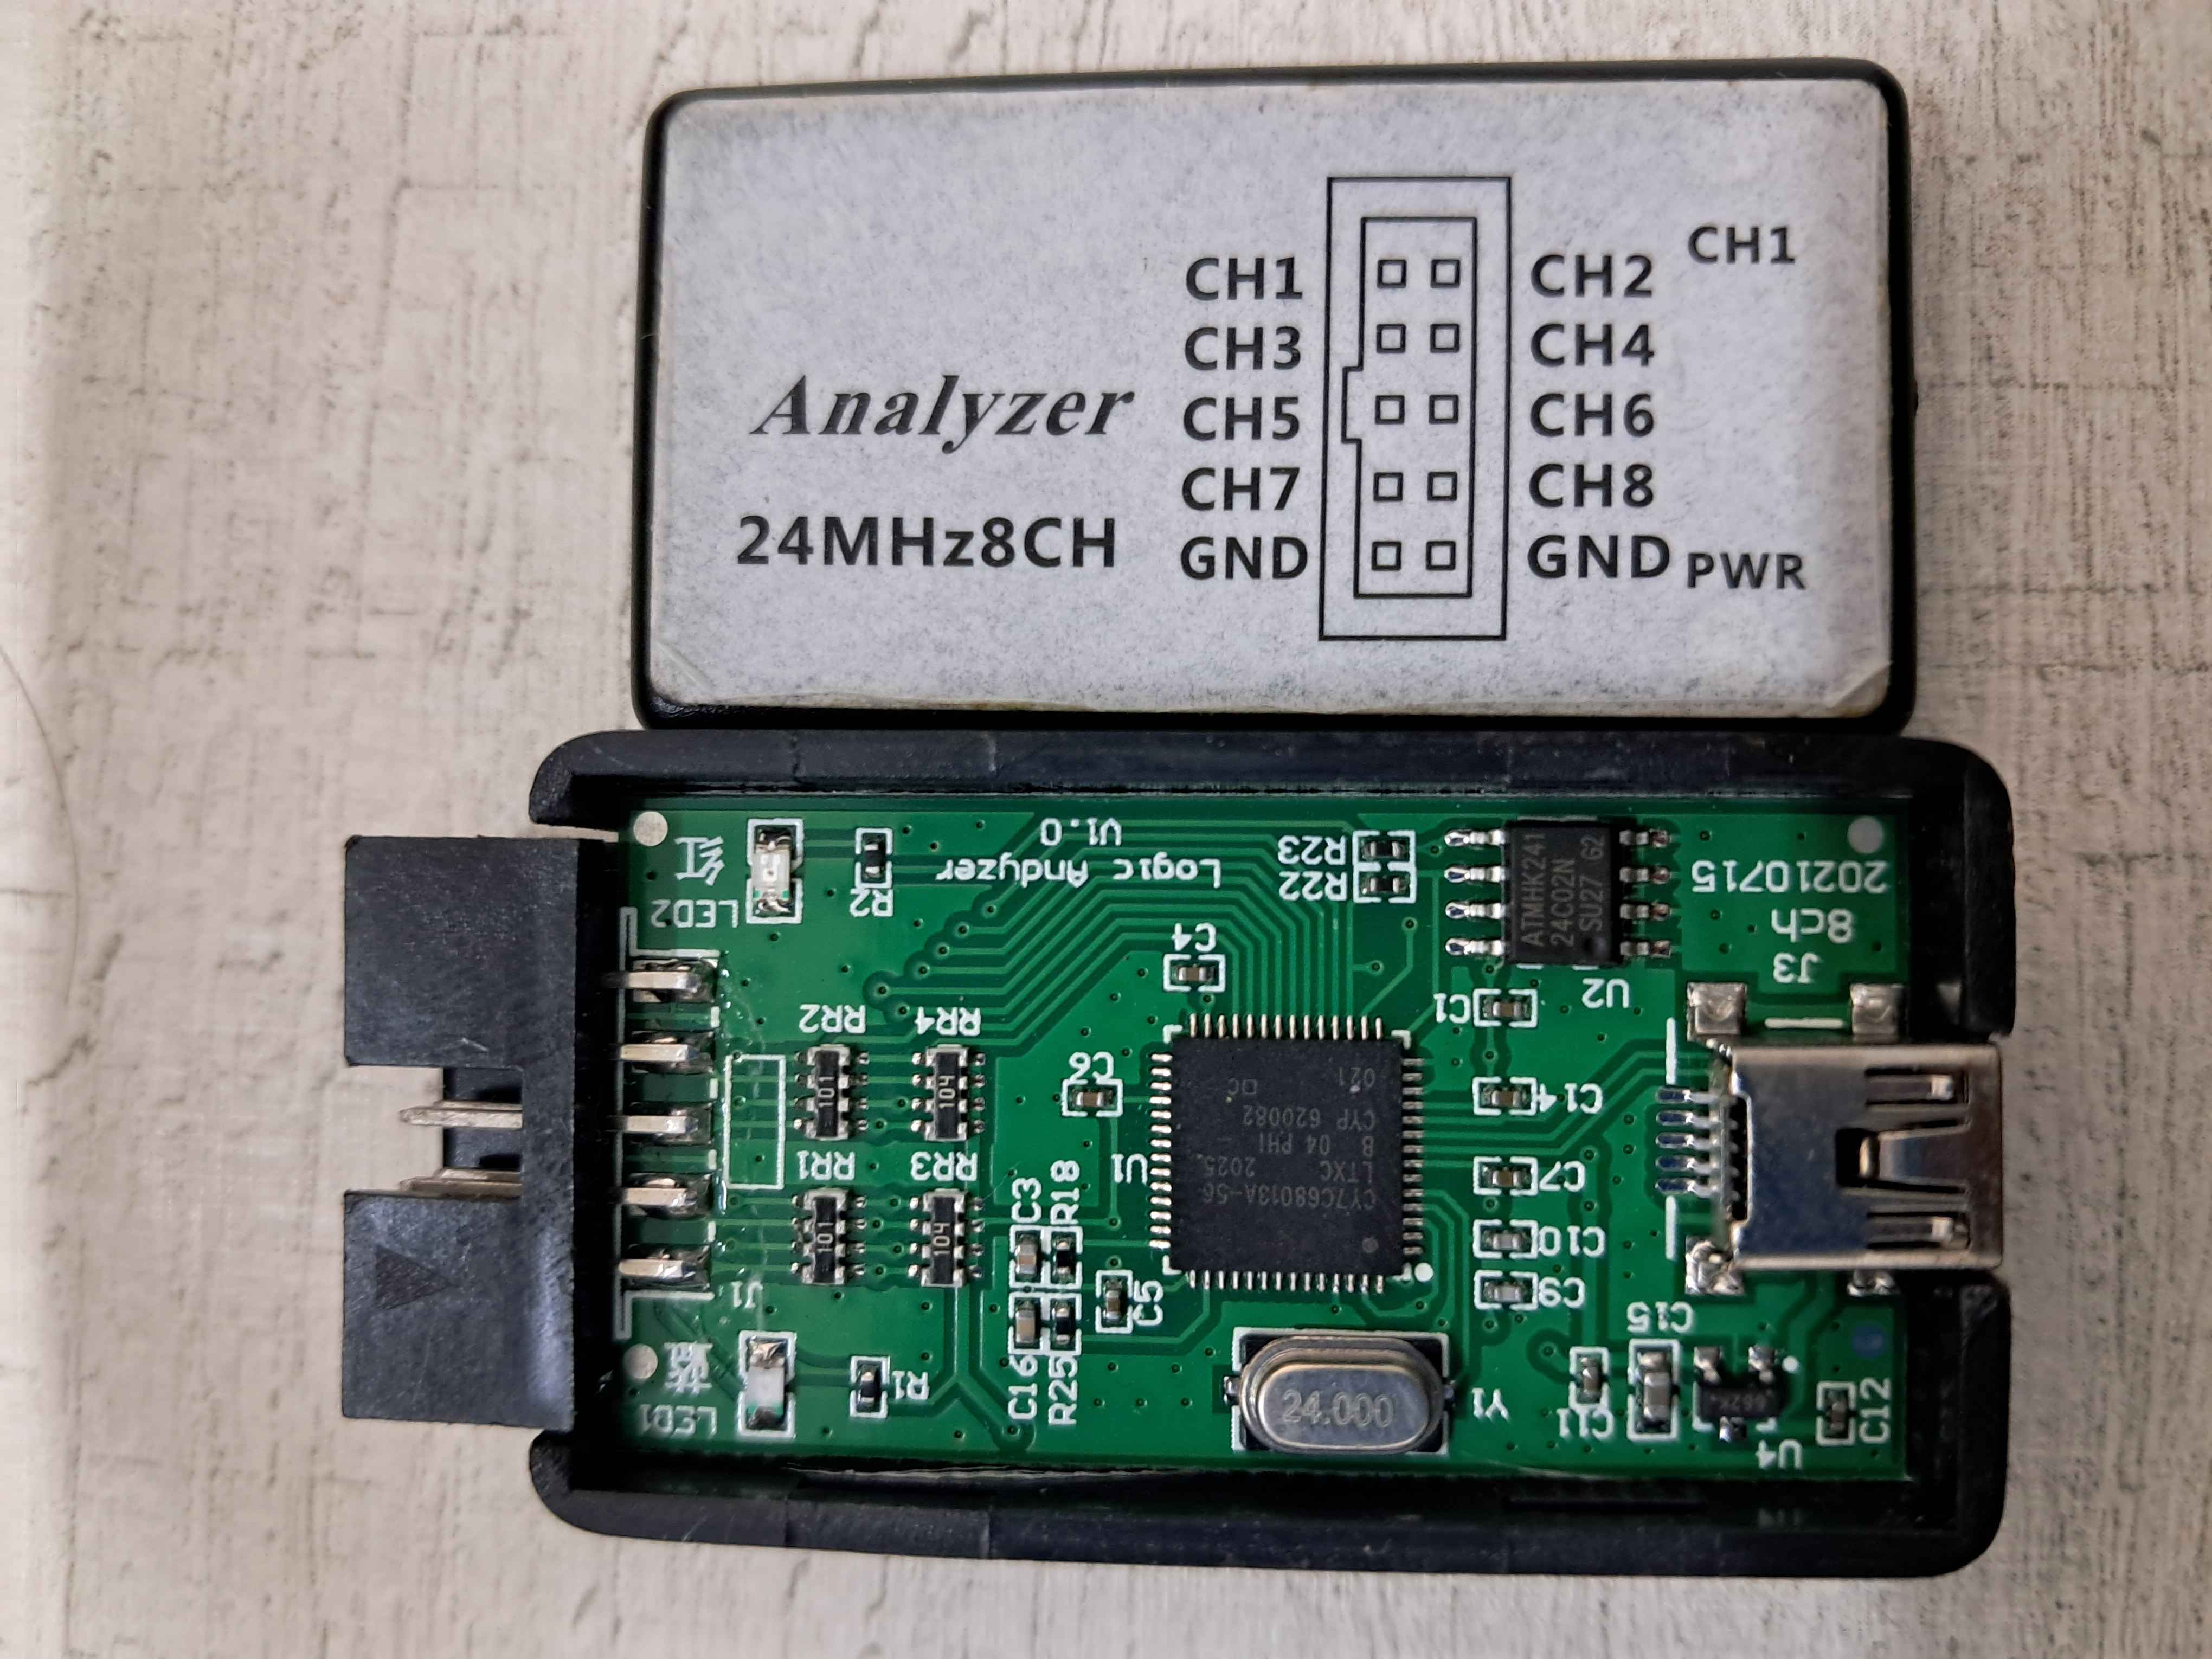
\includegraphics[width=0.5\linewidth]{Cap03/img/intrumento_ref.png}
    \fonte{Autoria própria.}
  \end{figure}

  \item \textbf{Host:} o mesmo computador para todas as medições, com os scripts em \texttt{benchmarks/} (Seção~\ref{sec:metricas}) controlando a captura via protocolo sigrok-pico (repetições, varreduras de taxa); versões fixadas e registradas.

  \item \textbf{Medição interna:} contador de ciclos \ac{DWT} (\texttt{DWT->CYCCNT}) do Cortex-M33 para ciclos por amostra e ocupação de \ac{CPU} \cite{arm2021}, exposto ao \emph{host} por um comando de protocolo dedicado (\texttt{'o'}, fora do conjunto sigrok-pico padrão) consultado por \texttt{benchmarks/m4\_cpu\_occupancy.py}. A perda de amostras não é contada no firmware: é medida no \emph{host}, a partir do fluxo entregue, e o transbordamento da fila de \emph{buffers} de A aparece ao \emph{host} como aborto da captura (\texttt{!!!}).

  \item \textbf{Análise:} scripts Python (diretório \texttt{benchmarks/} do repositório público do trabalho \cite{dias2026artefatos}) para contagem de bordas contra a referência, extração de períodos, histogramas de \emph{jitter} e estatística descritiva, de modo a viabilizar a repetibilidade integral do experimento por terceiros \cite{collberg2016}.
\end{itemize}

Antes das medições finais, a bancada foi validada executando M1 e M3 com
ambos os firmwares e comparando as capturas com a referência. Essa validação
revelou um defeito na primeira versão do Firmware A, que rearmava o \ac{PIO}
e o \ac{DMA} a cada bloco sem sinalizar a lacuna resultante; o defeito foi
corrigido, e todas as medições reportadas no Capítulo~\ref{cap:resultados}
usam a versão corrigida, descrita na Seção~\ref{sec:firmware-a}.

\section{Implementação dos firmwares}\label{sec:firmware}

Ambos os firmwares foram construídos sobre o Pico \ac{SDK}, em C
\emph{bare-metal}, e organizam-se em módulos: \ac{ADC}, captura, abstração de
\ac{PIO}/DMA ou \ac{GPIO}/CPU, protocolos sigrok, interfaces seriais e utilitários \ac{USB}
com \emph{TinyUSB}, distribuída com o \ac{SDK} \cite{rpi2024sdk}. A opção por
firmware \emph{bare-metal}, sem \ac{RTOS}, decorre de a temporização crítica
ser garantida pelo hardware (\ac{PIO}/DMA) e não por um escalonador de tarefas
(Seção~\ref{sec:hardware}); as \acp{API} leves do Pico \ac{SDK} (\texttt{pico\_time},
\texttt{hardware\_*}) oferecem acesso direto aos periféricos com sobrecusto
próximo de zero \cite{rpi2024sdk}. Os dois firmwares implementam o mesmo
conjunto de comandos do protocolo, resumido no Quadro~\ref{qua:comandos}.

\begin{quadro}[H]
  \centering
  \caption{Comandos do protocolo sigrok-pico.}
  \label{qua:comandos}
  \small
  \begin{tabularx}{\linewidth}{|l|>{\raggedright\arraybackslash}X|}
    \hline
    \textbf{Comando} & \textbf{Descrição}                             \\ \hline
    \texttt{i}       & Consulta de identificação                      \\ \hline
    \texttt{R}       & Define a taxa de amostragem (5\,kHz--120\,MHz em A; até $\approx 4{,}05$\,MHz em B) \\ \hline
    \texttt{L}       & Define o número de amostras (1--1.000.000)     \\ \hline
    \texttt{a}       & Consulta a escala do canal analógico           \\ \hline
    \texttt{A}       & Habilita/desabilita canal analógico            \\ \hline
    \texttt{D}       & Habilita/desabilita canal digital              \\ \hline
    \texttt{F}       & Captura de comprimento fixo                    \\ \hline
    \texttt{C}       & Captura contínua                               \\ \hline
    \texttt{t}       & Configura disparo                              \\ \hline
    \texttt{o}       & Consulta a ocupação de \acs{CPU} (extensão deste trabalho) \\ \hline
  \end{tabularx}
  \fonte{Autoria própria.}
\end{quadro}

\subsection{Firmware A (linha de base): aquisição por PIO+DMA}\label{sec:firmware-a}

\begin{figure}[htbp]
  \centering
  \caption{Arquitetura do Firmware A (PIO+DMA).}
  \label{fig:fw-a-arch}
  \vspace{-1cm}
  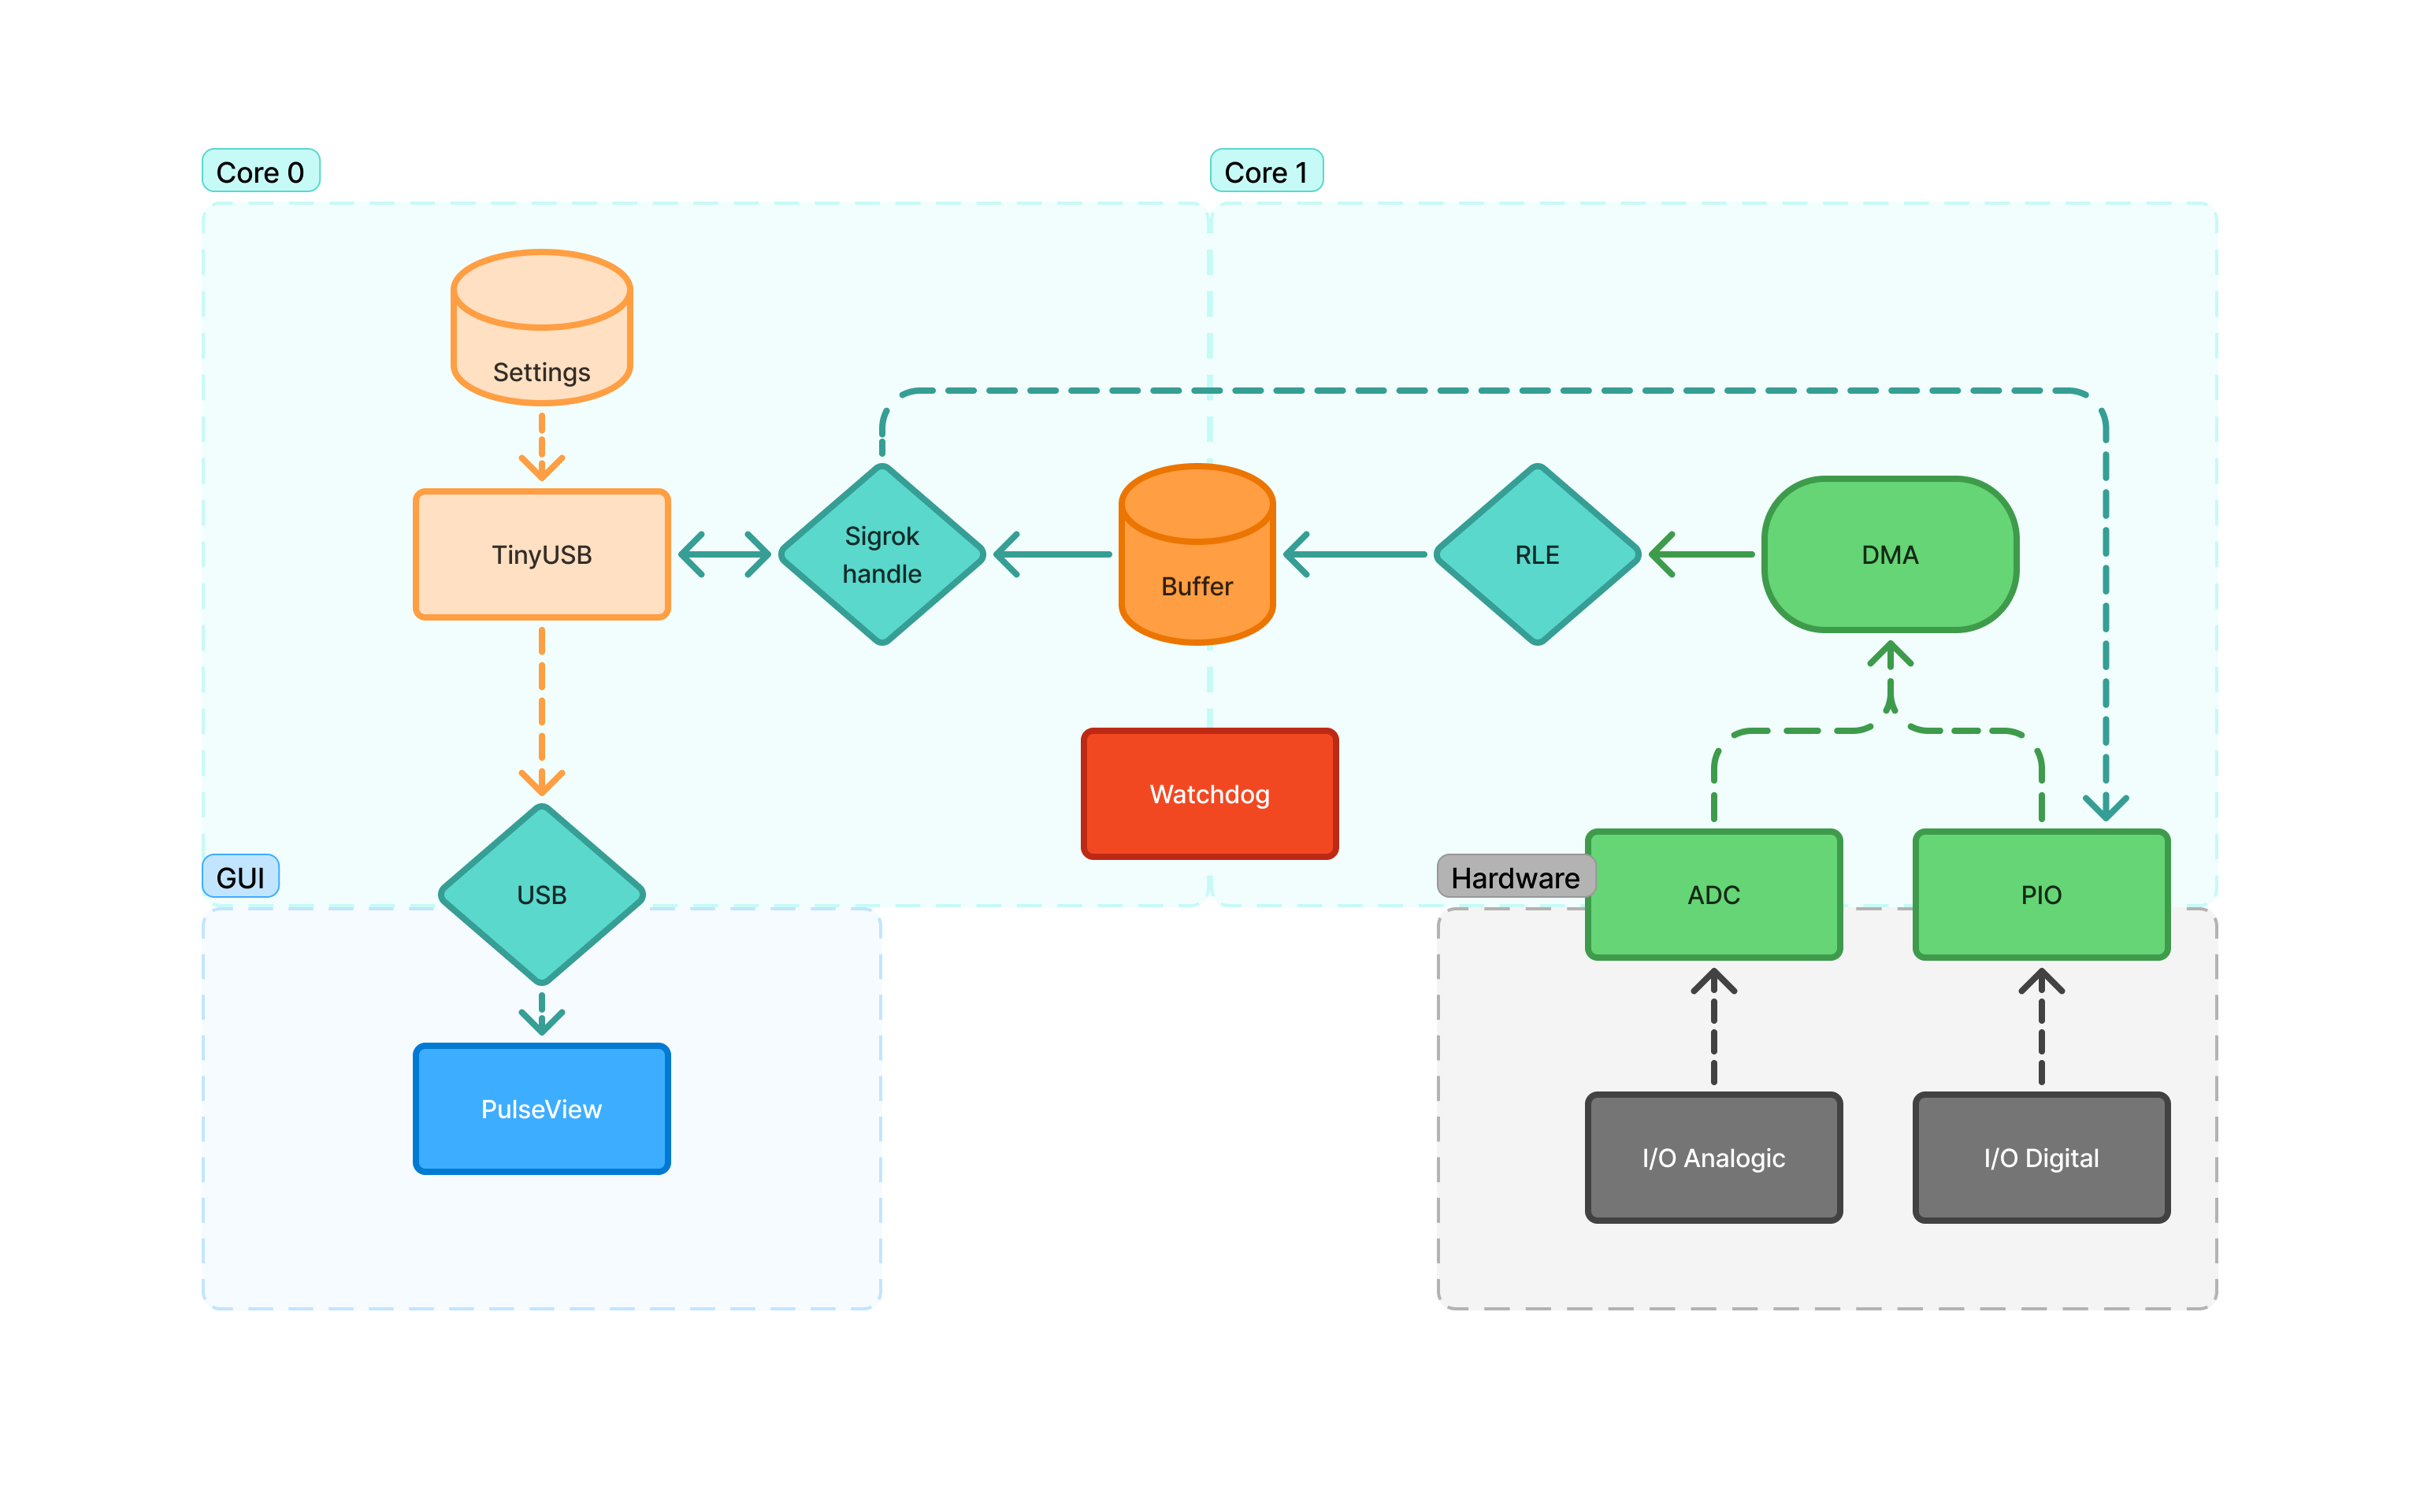
\includegraphics[width=1\linewidth]{Cap03/img/fw_A_arch.png}
  \vspace{-2cm}
  \fonte{Autoria própria.}
\end{figure}

O firmware A (Figura~\ref{fig:fw-a-arch}) implementa a amostragem inteiramente em hardware. Seis variantes
de programa \ac{PIO} são compiladas no binário: a mais simples executa em laço a
instrução \texttt{in pins, 12}, amostrando os doze canais digitais a cada ciclo
do clock da máquina de estados, com \emph{autopush} para o \ac{FIFO} a cada amostra
de 12 bits, que é o caminho de taxa máxima, com \emph{jitter} limitado ao divisor de
clock da máquina de estados (Equação~\ref{eq:clkdiv}). As demais
variantes antepõem ao laço de captura um estágio de espera baseado em
\texttt{jmp pin}, que monitora o \ac{GPIO} de disparo sem custo sobre a temporização
da captura subsequente, implementando disparo assistido por hardware (borda de
subida, borda de descida, qualquer borda, nível alto e nível baixo). Em todos
os casos, a taxa é programada pelo divisor de clock da máquina de estados
(Equação~\ref{eq:clkdiv}), cobrindo o intervalo de 5\,kHz a 120\,MHz exposto ao
\emph{host}.

O transporte das amostras também ocorre sem intervenção da \ac{CPU} no caminho
de cada amostra. Nas capturas apenas digitais, de comprimento fixo
(\texttt{F}) ou contínuas (\texttt{C}) e com ou sem disparo, dois canais de
\ac{DMA}, ritmados pelo \ac{DREQ} do \ac{FIFO} de recepção do \ac{PIO}, transferem as amostras
(unidades de 16 bits) para dois \emph{buffers} de 1\,024 amostras em \ac{SRAM} em
regime de \emph{ping-pong}: cada canal, ao completar seu \emph{buffer},
dispara o outro por encadeamento (\emph{chain}), de modo que a amostragem
nunca para; a interrupção de fim de bloco apenas contabiliza o \emph{buffer}
produzido e verifica se a \ac{CPU} já liberou o anterior. Se a \ac{CPU} ainda não tiver
consumido um \emph{buffer} quando o \ac{DMA} precisar reescrevê-lo, a fila de dois
\emph{buffers} transbordou: o firmware aborta a captura e envia ao \emph{host} o
marcador de erro \texttt{!!!} do protocolo, em vez de descartar amostras em
silêncio. Com disparo, o programa \ac{PIO} espera a condição via \texttt{jmp pin} e
só então entra no mesmo laço de amostragem, de forma que o disparo apenas
determina o início da captura. Na captura contínua, o \ac{DMA} é armado uma única
vez e o fluxo é fatiado nos blocos de $L$ amostras definidos pelo comando
\texttt{L}, cada um encerrado por um marcador com a contagem de \emph{bytes}
do bloco (\texttt{\$n+}), que permite ao \emph{host} verificar a completude. Apenas
as capturas com canais analógicos usam um caminho distinto, em que a \ac{CPU}
rearma o \ac{DMA} a cada bloco; esse caminho não é exercitado nos experimentos.
Em todos os casos, fora do caminho crítico de amostragem, a \ac{CPU} aplica \ac{RLE}
aos \emph{buffers} capturados, em que sequências de até 32 amostras idênticas
consecutivas colapsam em três \emph{bytes}, e os transmite ao \emph{host} via \ac{USB}
\ac{CDC} (TinyUSB).

Durante a captura, portanto, a \ac{CPU} permanece \textbf{fora do caminho de
  amostragem}: em nenhum dos dois modos ela lê os pinos ou conta ciclos por
amostra; seu papel se limita a monitorar \ac{DMA} e conexão \ac{USB} e, entre blocos,
codificar e transmitir os dados já amostrados, abortando a captura se o \emph{host}
desconectar. Essa é a propriedade arquitetural cujo valor este trabalho
quantifica.

\subsection{Firmware B: aquisição por GPIO+CPU}\label{sec:firmware-b}

\begin{figure}[htbp]
  \centering
  \caption{Arquitetura do Firmware B (GPIO+CPU).}
  \label{fig:fw-b-arch}
  \vspace{-1cm}
  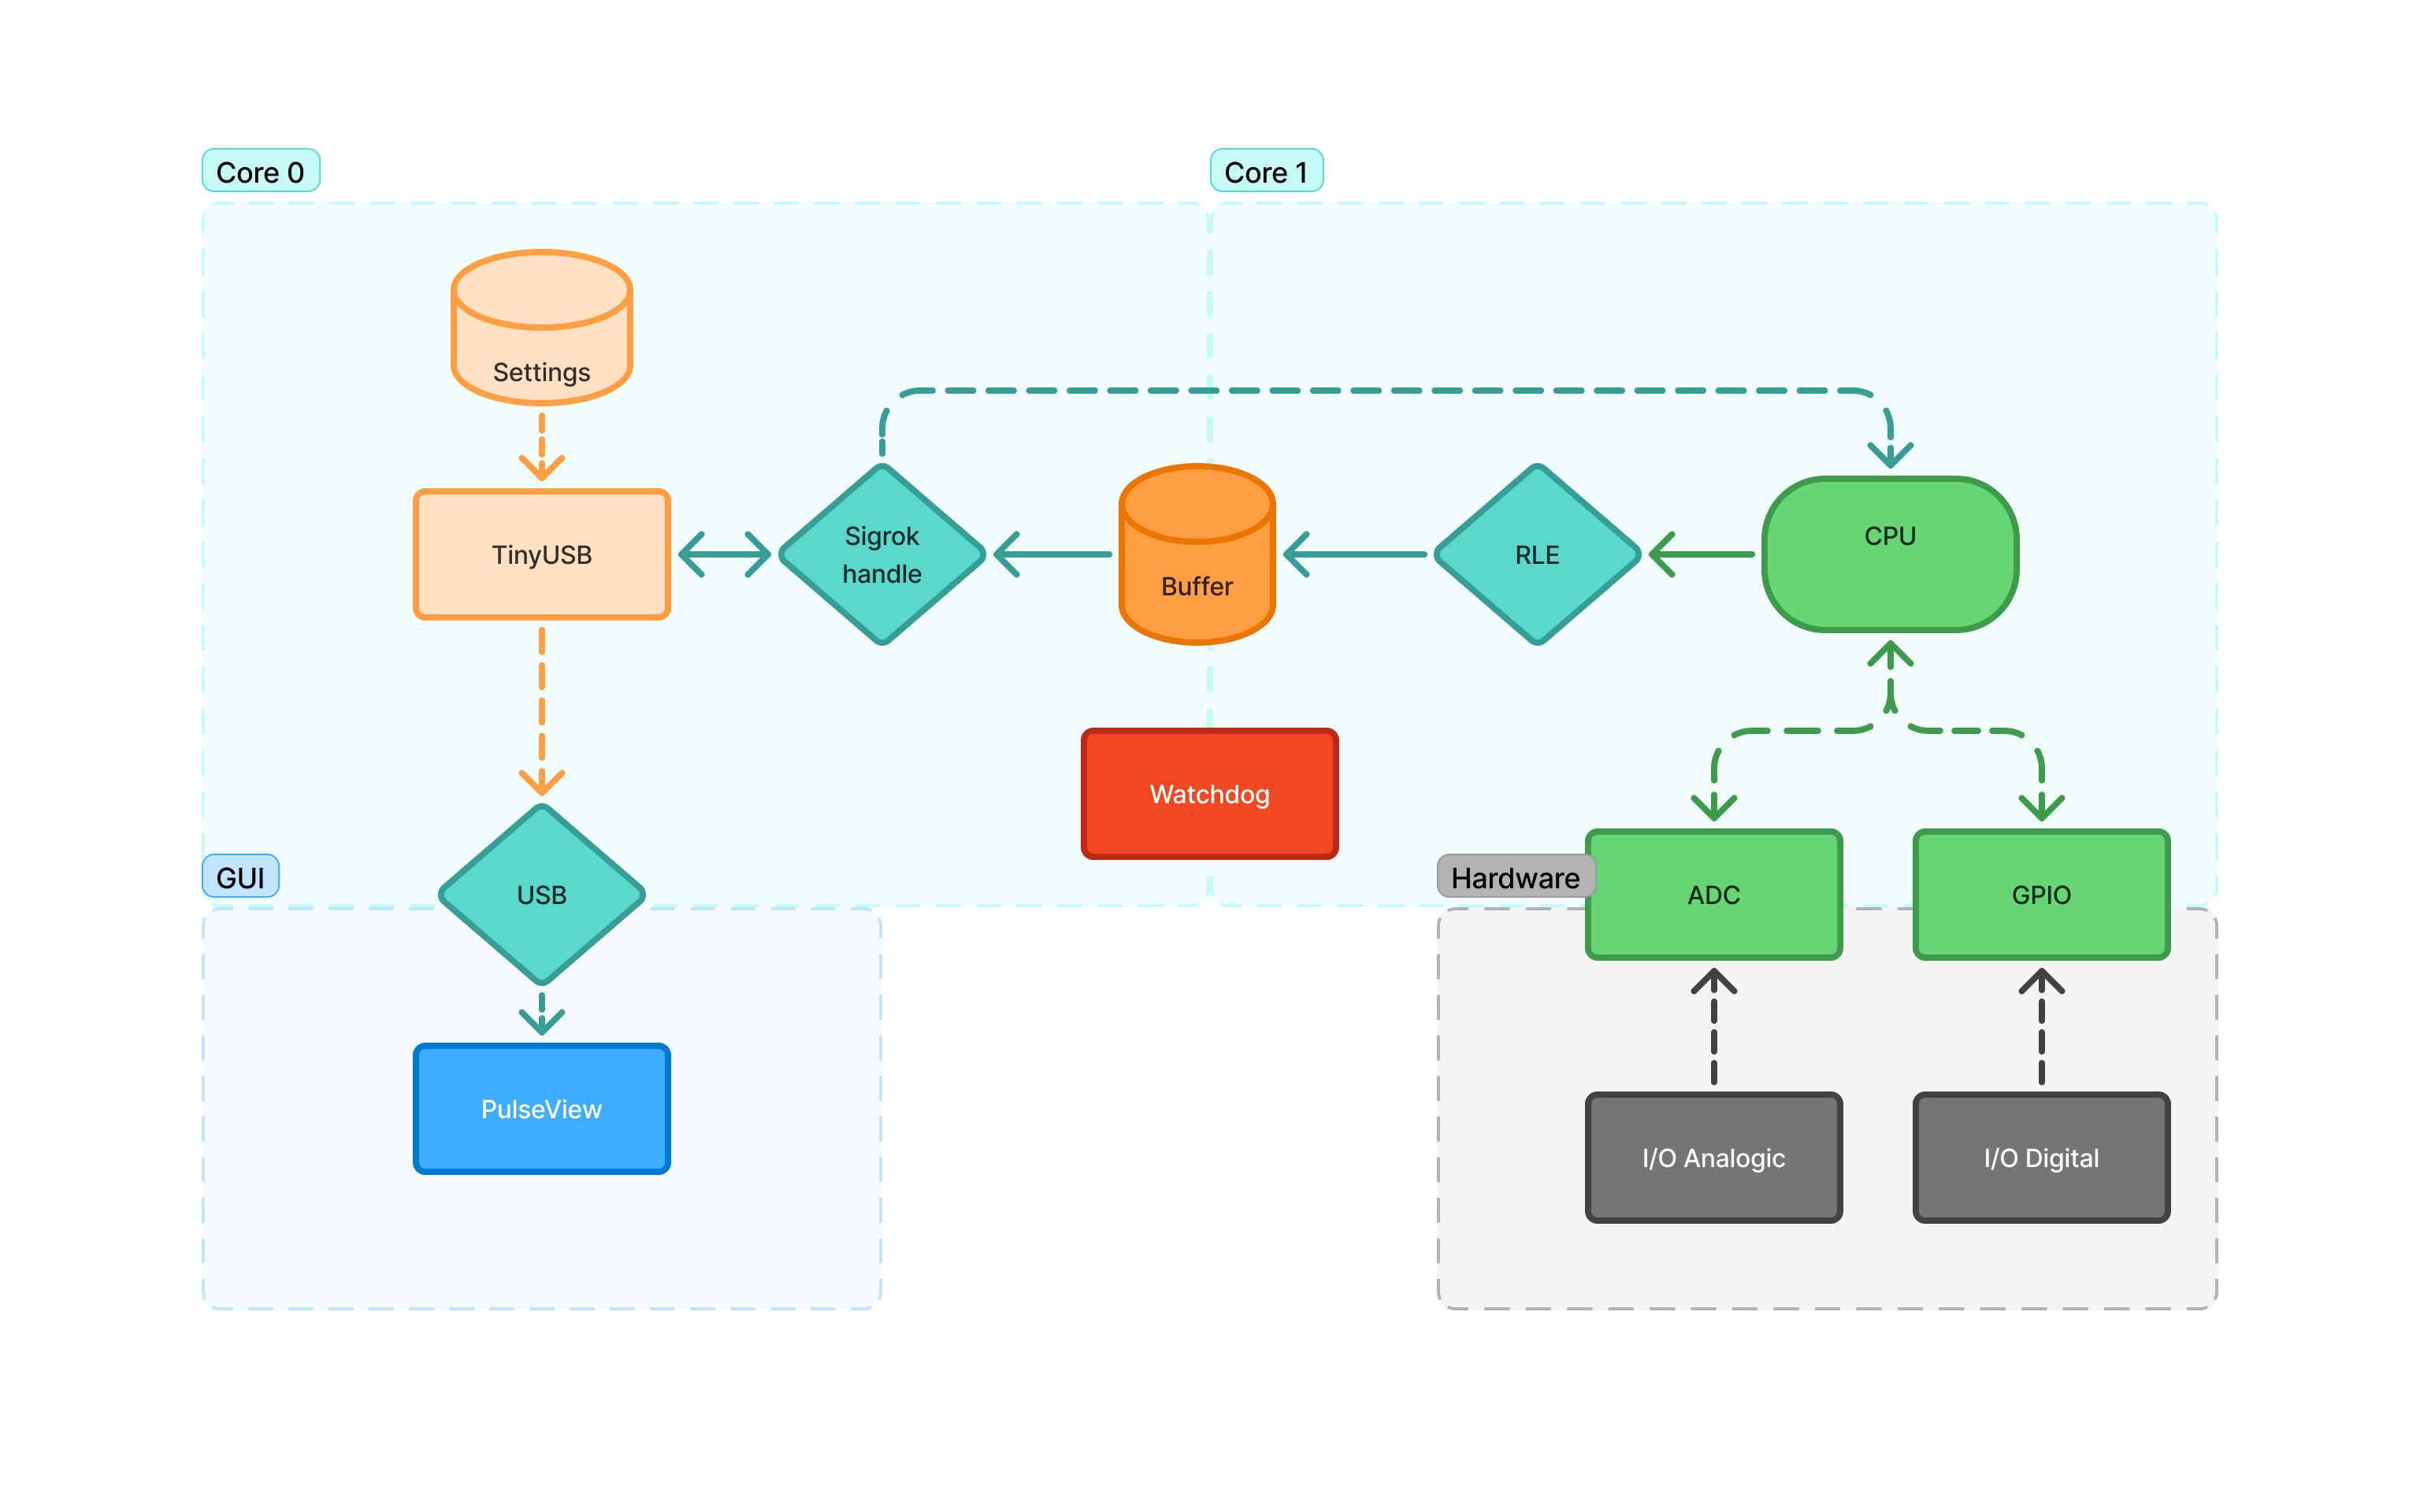
\includegraphics[width=1\linewidth]{Cap03/img/fw_B_arch.png}
  \vspace{-2cm}
  \fonte{Autoria própria.}
\end{figure}

O firmware B (Figura~\ref{fig:fw-b-arch}) substitui os estágios de amostragem e transporte do caminho de
dados por software, mantendo inalterados os estágios de codificação e
transmissão (\ac{RLE}, TinyUSB, protocolo, formato das amostras). As amostras são
obtidas pela leitura do registrador de entrada do bloco \ac{SIO}, no \ac{SDK}
\texttt{gpio\_get\_all()}, que retorna o estado de todos os \acp{GPIO} em uma
única leitura de 32 bits, da qual se extraem os 12 bits dos canais; essa é a
forma mais rápida de leitura de \ac{GPIO} disponível à \ac{CPU} no RP2350. O núcleo do
firmware é um laço apertado que lê o \ac{SIO}, armazena a amostra no buffer e
controla o período pelo contador de ciclos \texttt{CYCCNT} da unidade \ac{DWT}, que conta os
ciclos de $f_{clk}$: cada amostra espera o seu próprio prazo absoluto, obtido
somando o período ao prazo anterior, com a parte fracionária do período
acumulada em ponto fixo para que capturas longas não derivem. Assim, um atraso
eventual do laço atinge apenas a amostra em que ocorre, e as seguintes retomam
a grade de tempo, em vez de alongar todos os períodos. Na inicialização, o
firmware mede o custo de uma iteração do laço ($C_{iter}$) e recusa taxas que
exijam menos ciclos por amostra que esse custo acrescido de uma margem de
5\,\%. O laço é escrito em C e executado a partir da flash (\acs{XIP}), com as
interrupções habilitadas, como em uma aplicação convencional.

Uma variante adicional, prevista no projeto mas não avaliada nos experimentos
deste trabalho, explora os dois núcleos do RP2350: o núcleo 1 executa
exclusivamente o laço de amostragem, escrevendo em um buffer circular em \ac{SRAM},
enquanto o núcleo 0 executa TinyUSB, o protocolo e o \ac{RLE}, consumindo esse
buffer. A sincronização usa índices de escrita/leitura em posições de memória
distintas (produtor único/consumidor único), sem travas no caminho quente, e as
interrupções permanecem desabilitadas no núcleo 1 durante a captura. Todos
os resultados do Capítulo~\ref{cap:resultados} referem-se à variante de núcleo
único, em que o mesmo núcleo amostra, codifica e transmite.

O disparo por borda/nível, por sua vez, é implementado por comparação em
software no próprio laço (leitura, máscara e comparação com o estado anterior),
ao contrário do Firmware A, cujo disparo é assistido por hardware via \ac{PIO}
(Seção~\ref{sec:firmware-a}). Fora esses pontos, nada muda em relação ao
Firmware A: protocolo sigrok-pico, \ac{RLE}, TinyUSB e seus \emph{buffers}, clock do
sistema e placa são idênticos, e mudam apenas os mecanismos de amostragem e
transporte e, em consequência deles, o tamanho do par de \emph{buffers} de
amostras digitais: 1\,024 amostras cada no Firmware A e 8\,192 no Firmware B.
No Firmware B, a \ac{CPU} não amostra enquanto codifica e envia um bloco, de modo
que cada fronteira de bloco é uma pausa na amostragem; blocos maiores reduzem o
número dessas pausas e, portanto, favorecem o Firmware B na comparação. No
Firmware A, em que o \ac{DMA} continua amostrando durante o envio, o tamanho
original do projeto foi mantido. O firmware B é desenvolvido em \emph{branch}
dedicado do mesmo repositório, a partir do mesmo \emph{commit} base do firmware
A, com rastreabilidade por \emph{tag}.

\subsection{Ocupação de memória dos firmwares}\label{sec:fw-memoria}

A Tabela~\ref{tab:fw-memoria} compara o tamanho dos dois binários, obtido das
seções do arquivo \ac{ELF} gerado na compilação, em relação à flash de 2\,MB
declarada para a placa e aos 512\,KB de \ac{SRAM} principal do RP2350. A
diferença entre as duas versões concentra-se na seção de dados não
inicializados (\ac{BSS}), que abriga os \emph{buffers} de amostras.

\begin{table}[H]
  \centering
  \caption{Ocupação de memória dos Firmwares A e B.}
  \label{tab:fw-memoria}
  \begin{tabular}{@{}lrrr@{}}
    \toprule
    \textbf{Seção}                 & \textbf{Firmware A} & \textbf{Firmware B} & \textbf{B $-$ A} \\
    \midrule
    Código e constantes (flash)    & 51,7\,KB            & 46,2\,KB            & $-5{,}5$\,KB     \\
    Dados não inicializados (\acs{BSS})  & 109,2\,KB           & 225,3\,KB           & $+116{,}1$\,KB   \\
    \midrule
    Ocupação da flash (2\,MB)      & 2,5\,\%             & 2,3\,\%             & ---              \\
    Ocupação da \acs{SRAM} (512\,KB)     & 21,3\,\%            & 44,0\,\%            & ---              \\
    \bottomrule
  \end{tabular}
  \fonte{Autoria própria.}
  \nota{nenhum dos binários possui dados inicializados (\texttt{.data}) relevantes; 1\,KB = 1\,024 \emph{bytes}.}
\end{table}

Os dois binários ocupam uma fração pequena da flash. O Firmware A é 5,5\,KB
maior por embutir as seis variantes de programa \ac{PIO} e o código de configuração
e encadeamento do \ac{DMA}, que o Firmware B substitui por um laço único em C. Na
\ac{SRAM}, a relação se inverte: o Firmware B ocupa o dobro. Toda a diferença vem
dos \emph{buffers}: a constante de tamanho de bloco, elevada de 1\,024 para
8\,192 amostras, é compartilhada pelos pares de \emph{buffers} dos módulos
digital, RS-232 e RS-485 (seis \emph{buffers} de 2\,KB passam a 16\,KB, ou
84\,KB a mais), e o disparo por software de B mantém um histórico circular de
8\,192 palavras de 32 bits para as amostras de pré-disparo (32\,KB), que em A
é dispensado pelo disparo assistido pelo \ac{PIO}. As estruturas do TinyUSB e o
anel de transmissão \ac{USB} são idênticos nos dois. Mesmo com 44\,\% da \ac{SRAM}, o
Firmware B ainda cabe com folga no RP2350; o custo de memória, portanto, não
restringe a comparação, mas indica que a compensação adotada para B (blocos
maiores para reduzir as pausas de amostragem) é paga em \ac{SRAM}, recurso que o
Firmware A preserva.

\section{Métricas e procedimentos experimentais}\label{sec:metricas}

As métricas adotadas são quatro, definidas antes da coleta: taxa de amostragem máxima
sustentada, \emph{jitter} de amostragem, taxa de perda de amostras e ocupação
de \ac{CPU}. Restringir o conjunto a essas quatro grandezas, previamente definidas e
não selecionadas \emph{a posteriori}, evita diluir o orçamento experimental
(réplicas, tempo de bancada) em comparações que não sustentam o objetivo
geral do trabalho e reduz o risco de \emph{garden of forking paths} na análise
\cite{georges2007,mytkowicz2009}.

Cada métrica é executada com $N = 30$ repetições por ponto de medição, tamanho
amostral escolhido, conforme detalhado na Seção~\ref{sec:analise-estatistica},
por equilibrar a precisão dos intervalos de confiança e o tempo de bancada,
seguindo a prática de repetir as execuções e reportar a variabilidade
observada em vez de medições isoladas \cite{georges2007,kalibera2013},
reportando-se as estatísticas descritas
na Seção~\ref{sec:analise-estatistica}. Salvo indicação, varre-se a taxa de amostragem em passos logarítmicos
dentro da faixa suportada, interrompendo a varredura de cada firmware e
contagem de canais na primeira taxa em que o critério da métrica falha em
todas as repetições ou que o firmware recusa na configuração. Em M1, M2 e M3, o sinal é aplicado ao canal D3, e a
varredura é repetida com 4 e com 12 canais habilitados, contagens que
exercitam, respectivamente, um e dois \emph{bytes} por amostra no protocolo; em
M4, usam-se 1, 8 e 12 canais, com a onda de 1\,MHz aplicada aos canais, sinal
com muitas transições que exercita o custo da codificação \ac{RLE}, em capturas
curtas de 65\,536 amostras sem disparo, para que a medida reflita o custo de
processamento por amostra, e não o regime sustentado do \ac{USB}.

\paragraph{M1: Taxa máxima de amostragem sustentada.} A onda quadrada do gerador é aplicada ao canal D3 e ao
analisador lógico de referência, que fornece a contagem de bordas de
referência. Em taxa crescente, cada repetição arma um disparo por borda de
subida e mantém a janela de 0,2\,s seguinte. Enquanto a janela cabe no limite
de $10^6$ amostras do protocolo (até 3,66\,MS/s), a captura usa o modo de
quantidade fixa (\texttt{F}); acima disso, como em 5,39\,MS/s, o \emph{script}
usa o modo contínuo (\texttt{C}) armado na mesma borda e corta a janela no
\emph{host}. O \emph{script} do \emph{host} conta as bordas de subida no canal do
sinal. Sendo $n_{DAQ}$ o número de bordas contadas pelo \ac{DAQ} e $n_{ref}$
o contado pela referência na mesma janela, uma repetição é íntegra quando
(i) a janela inteira foi entregue sem erros de decodificação e sem aborto do
firmware e (ii)
\begin{equation}\label{eq:m1-integra}
  \left| n_{DAQ} - n_{ref} \right| \le \max\left(1;\ 0{,}001\, n_{ref}\right),
\end{equation}
isto é, a contagem coincide com a da referência dentro de 0,1\,\%, tolerância
que absorve a diferença entre a taxa solicitada e a efetivamente obtida. Taxas inferiores a
quatro amostras por período do sinal são excluídas, pois a subamostragem altera
a contagem sem representar falha de aquisição. A taxa máxima sustentada é a
maior taxa em que todas as $N$ repetições são íntegras:
\begin{equation}\label{eq:m1-fmax}
  f_{s,\mathrm{sust}} = \max \left\{ f_s \;:\; \text{as } N \text{ repetições em } f_s \text{ satisfazem a Equação~\ref{eq:m1-integra}} \right\}.
\end{equation} Como análise de sensibilidade
secundária, repete-se a mesma classificação com tolerância de $\pm 2$ bordas,
o mínimo que absorve o corte da janela, para verificar se a conclusão
depende da tolerância escolhida. Comparam-se A e B, e o
resultado de B é confrontado com o teto teórico $f_{clk}/C_{iter}$
(Equação~\ref{eq:fsmax}), com $C_{iter}$ medido por \ac{DWT}.

\paragraph{M2: \emph{Jitter} de amostragem.} Captura, com disparo e janela de 0,2\,s, da onda quadrada de
100\,kHz (frequência aferida pelo instrumento de referência), em taxas de 2,0 a
4,05\,MS/s, e análise da distribuição dos períodos medidos entre bordas de
subida consecutivas. Sendo $i_k$ o índice da $k$-ésima borda de subida e
$T_s = 1/f_s$ o período de amostragem, o $k$-ésimo período medido é
\begin{equation}\label{eq:m2-periodo}
  \tau_k = (i_{k+1} - i_k)\, T_s ,
\end{equation}
e reportam-se, por taxa e por firmware, o desvio-padrão $\sigma$ e o valor
pico a pico $\max_k \tau_k - \min_k \tau_k$ dos períodos da janela.

Como o período do sinal raramente é múltiplo inteiro de $T_s$, o intervalo
entre bordas alterna entre $\lfloor P \rfloor$ e $\lceil P \rceil$ amostras,
com $P = f_s/f_{sig}$. Mesmo um amostrador ideal apresenta, portanto, um
desvio-padrão de quantização
\begin{equation}\label{eq:jitter-quant}
  \sigma_q = T_s \sqrt{\varphi\,(1-\varphi)}, \qquad \varphi = P - \lfloor P \rfloor ,
\end{equation}
e apenas o excedente
\begin{equation}\label{eq:jitter-exc}
  \sigma_{exc} = \sqrt{\sigma^2 - \sigma_q^2}
\end{equation}
pode ser atribuído à instabilidade do instante de amostragem. Como $\varphi$
depende da razão exata entre $f_s$ e $f_{sig}$, $\sigma_q$ varia de forma não
monotônica com a taxa. A mesma captura fornece ainda a diferença
$\Delta n = n_{DAQ} - n_{ref}$ entre os números de períodos contados pelo
\ac{DAQ} e pela referência.

\paragraph{M3: Captura contínua e perda de amostras.} Captura contínua (\texttt{C}) da onda quadrada de 100\,kHz com transmissão
simultânea ao \emph{host} por $T = 60$\,s, em taxas a partir de 1,09\,MS/s (abaixo
dela, o período tem menos de oito amostras e a detecção de lacunas perde
sensibilidade). A medida principal é a fração entregue
\begin{equation}\label{eq:m3-fracao}
  \eta = \frac{N_{ent}}{f_s \, T},
\end{equation}
em que $N_{ent}$ é o número de amostras recebidas pelo \emph{host}. Registram-se
também a taxa efetiva, os abortos sinalizados pelo firmware e o número de
lacunas, detectadas quando o intervalo entre bordas consecutivas se afasta do
período nominal $P = f_s/f_{sig}$, em amostras, por mais de 1,5 amostra:
\begin{equation}\label{eq:m3-lacuna}
  \left| (i_{k+1} - i_k) - P \right| > 1{,}5 .
\end{equation} Como o sinal é
periódico, uma lacuna que dure um número inteiro de períodos não é detectada
pelo intervalo entre bordas; a fração entregue é, por isso, a medida principal
de perda, e o número de lacunas, um limite inferior. Este é o experimento que
expõe o conflito amostragem$\times$\ac{USB}.

Como ensaio auxiliar, para separar o limite do barramento do limite do
firmware, mede-se também a vazão \ac{USB} em captura contínua com sinal pouco
compressível (onda de 1\,MHz), de 0,5 a 4\,MS/s, com 4 e 12 canais, em
capturas de 5\,s com três repetições por condição. O \emph{host} registra os
\emph{bytes} recebidos por segundo e a fração de amostras entregue. Por ter
caráter apenas descritivo, esse ensaio não entra na análise estatística.

\paragraph{M4: Ocupação de CPU.} Mede-se, via contador de ciclos \ac{DWT} (\texttt{DWT->CYCCNT}), a fração de ciclos
que a \ac{CPU} permanece ocupada durante a captura, em cada taxa e contagem de
canais:
\begin{equation}\label{eq:m4-ocupacao}
  O = \frac{C_{ocup}}{C_{total}},
\end{equation}
em que $C_{total}$ é o número de ciclos decorridos na captura e $C_{ocup}$, o
número de ciclos contados como ocupados. O que conta como ocupado difere entre os firmwares e decorre da
própria arquitetura: no Firmware A, contam-se apenas os trechos de
codificação \ac{RLE} e transmissão de cada \emph{buffer}, e não a espera pela
\ac{DMA}, já que nela a \ac{CPU} estaria livre para outra tarefa; no Firmware B,
conta-se a captura inteira, porque a \ac{CPU} está no caminho de cada amostra.
Espera-se, em A, ocupação baixa, limitada ao custo de codificar e transmitir
e crescente com a taxa; em B, ocupação próxima de 100\,\% em qualquer taxa. Esta é a métrica que
quantifica diretamente a propriedade arquitetural central do trabalho, isto é, a \ac{CPU}
permanecer ou não fora do caminho de dados (Seção~\ref{sec:firmware-a}).

\section{Análise estatística}\label{sec:analise-estatistica}

Para cada uma das quatro métricas (M1--M4), em cada condição (taxa de
amostragem $\times$ contagem de canais), reportam-se a mediana das
repetições nas tabelas e a média com o mínimo e o máximo nas figuras. Seguindo as recomendações da literatura de
avaliação estatisticamente rigorosa de desempenho de sistemas computacionais
\cite{georges2007,hoefler2015,fleming1986}, a comparação entre Firmware A e
Firmware B na mesma condição segue um procedimento fixo, definido a priori, e
não uma escolha \emph{ad hoc} por métrica:

\begin{itemize}
  \item \textbf{Teste de hipótese.} Para cada condição, testa-se
        $H_0$: as distribuições de A e B não diferem, contra $H_1$: diferem, com o
        teste não paramétrico de Mann--Whitney U ($\alpha = 0{,}05$), aplicado
        sempre, e não apenas ``quando pertinente'', em razão da ausência de
        suposição de normalidade sobre as distribuições das métricas
        \cite{georges2007}.

  \item \textbf{Tamanho de efeito.} Significância estatística não implica
        relevância prática: em medições de bancada com baixa dispersão,
        diferenças pequenas em termos absolutos podem produzir p-valores
        muito baixos, de modo que o p-valor isolado pouco informa sobre a
        magnitude da diferença observada
        \cite{fleming1986,hoefler2015}. Reporta-se, portanto, junto a cada teste,
        o tamanho de efeito pela correlação \emph{rank-biserial} $r$
        (equivalente ao $\delta$ de Cliff), permitindo distinguir diferença estatisticamente detectável de
        diferença relevante em magnitude.

  \item \textbf{Correção para comparações múltiplas.} A varredura de taxas
        combinada às contagens de canais gera múltiplos testes pareados por
        métrica. Para cada métrica (M1, M2, M3 e M4 tratadas como famílias
        separadas), aplica-se a correção de Holm--Bonferroni sobre o conjunto de
        comparações daquela métrica; o texto reporta o p-valor ajustado
        ($p_{\mathrm{Holm}}$), e os p-valores brutos acompanham os dados no
        repositório público do trabalho \cite{dias2026artefatos}.

  \item \textbf{Intervalo de confiança.} Além das estatísticas descritivas,
        reporta-se o \ac{IC} de 95\,\% para a diferença de medianas
        entre A e B, obtido por \emph{bootstrap} percentil (10.000 reamostragens)
        \cite{kalibera2013}, mais informativo que mínimo e máximo para caracterizar
        a incerteza da estimativa.

  \item \textbf{Justificativa do tamanho amostral.} Adota-se $N = 30$
        repetições por ponto de medição, valor acima do mínimo estritamente exigido
        pelo Mann--Whitney U para significância exata e alinhado à prática de
        benchmarking rigoroso de sistemas, em que amostras da ordem de dezenas por
        condição são recomendadas para estabilizar a estimativa de variância entre
        execuções e sustentar a aproximação assintótica usada pelo teste e pelo
        \emph{bootstrap} \cite{kalibera2013,georges2007,mytkowicz2009}. O
        compromisso remanescente com o tempo de bancada, e a limitação de poder
        estatístico que ele ainda impõe para efeitos pequenos, é tratado na
        ameaça à validade de conclusão (Seção~\ref{sec:limitacoes}).
\end{itemize}

Resultados são apresentados em tabelas, com medianas e os testes acima, e em
gráficos que mostram a média de cada condição com barras do mínimo ao máximo
das repetições; todos os testes são calculados com
\texttt{scipy.stats.mannwhitneyu}, e todos os dados brutos e scripts de análise
(incluindo o cálculo de tamanho de efeito, correção de Holm--Bonferroni e
\emph{bootstrap}) são versionados no diretório \texttt{benchmarks/}
(\texttt{stats.py} e \texttt{compare.py}) do repositório público do trabalho
\cite{dias2026artefatos}, para reprodutibilidade.

\cleardoublepage
% % % % % % % % % % % % % % % % % % % % % % % % % % %
\chapter{Resultados e Discussões}\label{cap:resultados}

Este capítulo apresenta e discute os resultados obtidos para as quatro
métricas definidas na Seção~\ref{sec:metricas}: taxa máxima de
amostragem sustentada (M1, Seção~\ref{sec:res-m1}), \emph{jitter} de
amostragem (M2, Seção~\ref{sec:res-m2}), perda de amostras em captura
contínua (M3, Seção~\ref{sec:res-m3}) e ocupação de \ac{CPU} (M4,
Seção~\ref{sec:res-m4}). O capítulo
encerra com uma síntese (Seção~\ref{sec:res-sintese}) que confronta os
resultados com o comportamento esperado de cada arquitetura
(Capítulo~\ref{cap:fundamentacao}).

\section{Visão geral}

O Quadro~\ref{qua:metricas} resume as quatro métricas avaliadas, a unidade
em que cada uma é reportada, o instrumento que a fornece e as equações que a
definem na Seção~\ref{sec:metricas}.

\begin{quadro}[H]
  \centering
  \caption{Resumo das métricas de comparação.}
  \label{qua:metricas}
  \begin{tabularx}{\linewidth}{|l|>{\raggedright\arraybackslash}p{2.9cm}|>{\raggedright\arraybackslash}p{2.4cm}|>{\raggedright\arraybackslash}X|l|}
    \hline
    \textbf{\#} & \textbf{Métrica}            & \textbf{Unidade}         & \textbf{Instrumento principal} & \textbf{Eq.} \\ \hline
    M1          & Taxa máxima sustentada      & MSa/s                     & Onda de referência + contagem de bordas (analisador lógico) & \ref{eq:m1-integra}, \ref{eq:m1-fmax} \\ \hline
    M2          & \emph{Jitter} de amostragem & ns ($\sigma$, p-p)       & Onda de referência + analisador lógico & \ref{eq:m2-periodo}--\ref{eq:jitter-exc} \\ \hline
    M3          & Perda em captura contínua   & \% amostras; lacunas/min & Onda de referência + detecção de lacunas e abortos & \ref{eq:m3-fracao}, \ref{eq:m3-lacuna} \\ \hline
    M4          & Ocupação de \acs{CPU}             & \% de ciclos ocupados    & Contador de ciclos \acs{DWT} & \ref{eq:m4-ocupacao} \\ \hline
  \end{tabularx}
  \fonte{Autoria própria.}
\end{quadro}

Em todas as figuras, cada ponto é a média das $N = 30$ repetições da
condição, e a faixa sombreada e as barras vão do menor ao maior valor
observado entre as repetições; o Firmware A é
representado em azul com linha contínua e círculos, e o Firmware B em laranja
com linha tracejada e quadrados. Nas tabelas, $p_{\mathrm{Holm}}$ é o p-valor
do teste de Mann--Whitney U ajustado por Holm--Bonferroni dentro da família
da métrica, e $r$ é a correlação \emph{rank-biserial}, com $r > 0$ indicando
valores maiores em B (Seção~\ref{sec:analise-estatistica}).

As condições de cada ensaio (sinal de 100\,kHz no canal D3, 4 e 12 canais
habilitados em M1--M3, janela de 0,2\,s em M1 e M2, captura de 60\,s em M3)
estão descritas na Seção~\ref{sec:metricas}.

\section{M1: Taxa máxima de amostragem sustentada}\label{sec:res-m1}

\subsection{Resultado}

O ensaio usou onda quadrada de 100\,kHz ($f_{sig} = 99{\,}999{,}83$\,Hz
segundo o analisador de referência), de modo que a varredura começa em $4 f_{sig} \approx
400$\,kS/s e prossegue em passos logarítmicos até a primeira taxa em que
alguma repetição falha. A Tabela~\ref{tab:m1-resumo} e a
Figura~\ref{fig:m1-integras} resumem o resultado.

\begin{table}[H]
  \centering
  \caption{M1: repetições íntegras e bordas contadas por taxa.}
  \label{tab:m1-resumo}
  \small
  \begin{tabular}{@{}llrrrr@{}}
    \toprule
    \textbf{Firmware} & \textbf{Canais} & \textbf{Taxa (kS/s)} &
    \textbf{Íntegras} & \textbf{Bordas \acs{DAQ} (mediana)} &
    \textbf{Excesso} \\
    \midrule
    A & 4  & 525,5    & 30/30 & 19\,999 & $-1$ \\
    A & 4  & 774,6    & 30/30 & 19\,999 & $-1$ \\
    A & 4  & 1\,141,7 & 30/30 & 19\,999 & $-1$ \\
    A & 4  & 1\,682,7 & 30/30 & 19\,999 & $-1$ \\
    A & 4  & 2\,480,2 & 30/30 & 20\,000 & $0$  \\
    A & 4  & 3\,655,6 & 30/30 & 20\,000 & $0$  \\
    A & 4  & 5\,388,0 & 0/30  & ---     & ---  \\
    A & 12 & 525,5    & 30/30 & 19\,999 & $-1$ \\
    A & 12 & 774,6    & 30/30 & 19\,999 & $-1$ \\
    A & 12 & 1\,141,7 & 30/30 & 20\,000 & $0$  \\
    A & 12 & 1\,682,7 & 30/30 & 19\,999 & $-1$ \\
    A & 12 & 2\,480,2 & 30/30 & 20\,000 & $0$  \\
    A & 12 & 3\,655,6 & 30/30 & 20\,000 & $0$  \\
    A & 12 & 5\,388,0 & 0/30  & ---     & ---  \\
    \midrule
    B & 4  & 525,5    & 30/30 & 19\,999 & $-1$  \\
    B & 4  & 774,6    & 30/30 & 20\,000 & $0$   \\
    B & 4  & 1\,141,7 & 30/30 & 20\,008 & $+8$  \\
    B & 4  & 1\,682,7 & 30/30 & 20\,010 & $+10$ \\
    B & 4  & 2\,480,2 & 30/30 & 20\,008 & $+8$  \\
    B & 4  & 3\,655,6 & 0/30  & 20\,028 & $+28$ \\
    B & 12 & 525,5    & 30/30 & 20\,001 & $+1$  \\
    B & 12 & 774,6    & 30/30 & 20\,000 & $0$   \\
    B & 12 & 1\,141,7 & 30/30 & 20\,003 & $+3$  \\
    B & 12 & 1\,682,7 & 30/30 & 20\,003 & $+3$  \\
    B & 12 & 2\,480,2 & 30/30 & 20\,005 & $+5$  \\
    B & 12 & 3\,655,6 & 0/30  & 20\,029 & $+29$ \\
    \bottomrule
  \end{tabular}
  \fonte{Autoria própria.}
  \nota{medianas de 30 repetições; janela de 0,2\,s; a referência registra 20\,000 bordas de subida por janela; excesso = bordas do DAQ $-$ bordas da referência. Em A a 5\,388,0\,kS/s, a captura é abortada pelo firmware.}
\end{table}

\begin{figure}[htbp]
  \centering
  \caption{M1: repetições íntegras por taxa de amostragem.}
  \label{fig:m1-integras}
  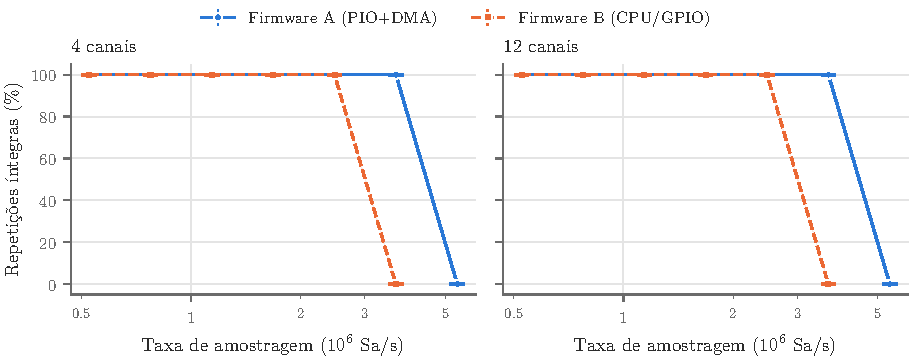
\includegraphics[width=\linewidth]{Cap04/img/m1_integras.pdf}
  \fonte{Autoria própria.}
\end{figure}

Pelo critério da Seção~\ref{sec:metricas} (tolerância de 0,1\,\% na
contagem), a taxa máxima sustentada do Firmware A é 3\,655,6\,kS/s e a do
Firmware B é 2\,480,2\,kS/s, tanto com 4 quanto com 12 canais. Os dois
firmwares, porém, falham de modos diferentes. Em A, a contagem de bordas
coincide com a da referência, a menos do corte da janela ($\pm 1$ borda),
em todas as repetições até 3\,655,6\,kS/s; na taxa seguinte, o firmware
detecta o transbordamento do \emph{buffer} e aborta a captura com o
marcador \texttt{!!!} do protocolo depois de entregar um único
\emph{buffer} de 1\,024 amostras. Em B, a captura nunca é abortada, mas o
\ac{DAQ} registra mais bordas do que a referência, e o excesso cresce com a taxa
(Figura~\ref{fig:m1-excesso}): a contagem é exata até 774,6\,kS/s, passa
a ter de 3 a 10 bordas a mais a partir de 1\,141,7\,kS/s, ainda dentro da
tolerância de 20 bordas, e salta para cerca de 28 bordas em
3\,655,6\,kS/s, quando todas as repetições falham.

\begin{figure}[htbp]
  \centering
  \caption{M1: excesso de bordas do DAQ em relação à referência.}
  \label{fig:m1-excesso}
  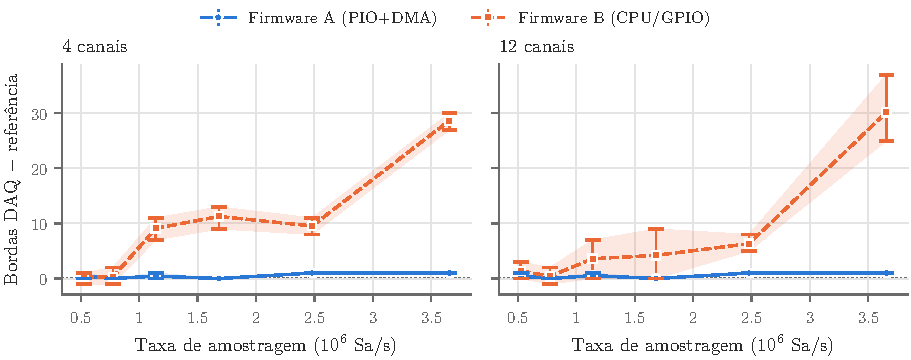
\includegraphics[width=\linewidth]{Cap04/img/m1_excesso_bordas.pdf}
  \fonte{Autoria própria.}
  \nota{repetições abortadas excluídas.}
\end{figure}

Bordas \emph{a mais} não podem vir de amostras perdidas em sequência
contínua; indicam que as amostras entregues cobrem um intervalo de tempo
maior que o nominal, isto é, que a amostragem foi interrompida e retomada
sem que o fluxo sinalizasse a interrupção. Uma pausa mais curta que meio
período do sinal não apaga bordas, mas desloca as seguintes; cada retomada
ocorre em fase arbitrária da onda, e o acúmulo dessas pausas faz a janela
de amostras se estender além de 0,2\,s e conter bordas extras. Esse é o
comportamento esperado de B quando o laço de amostragem é atrasado pelo
envio do bloco anterior. Se o critério de tolerância fosse reduzido a
$\pm 2$ bordas, suficiente para absorver o corte da janela, a taxa
sustentada de A não mudaria, enquanto a de B cairia para 774,6\,kS/s.

A comparação estatística usa a contagem de bordas de cada repetição nas
doze condições medidas pelos dois firmwares, de 525,5 a 3\,655,6\,kS/s
(Tabela~\ref{tab:m1-estat}). A partir de 1\,141,7\,kS/s, B conta mais
bordas que A em todas as condições, com separação completa ou quase
completa entre as repetições ($r \ge +0{,}90$): a diferença de medianas
vai de 2 a 12 bordas até 2\,480,2\,kS/s e chega a 27 a 30 bordas em
3\,655,6\,kS/s. Em 525,5 e 774,6\,kS/s a diferença é de no máximo duas
bordas e só é significativa em 525,5\,kS/s com 12 canais, ainda assim
dentro do corte da janela e sem relevância prática.

\begin{table}[H]
  \centering
  \caption{M1: comparação estatística da contagem de bordas (B $-$ A).}
  \label{tab:m1-estat}
  \begin{tabular}{@{}rrrrr@{}}
    \toprule
    \textbf{Canais} & \textbf{Taxa (kS/s)} & $\boldsymbol{r}$ &
    $\boldsymbol{p_{\mathrm{Holm}}}$ & \textbf{IC 95\,\% (bordas)} \\
    \midrule
    4 & 525{,}5 & $-0{,}14$ & $3{,}1 \times 10^{-1}$ & $[-1; 1]$ \\
    4 & 774{,}6 & $+0{,}20$ & $2{,}6 \times 10^{-1}$ & $[0; 1]$ \\
    4 & 1\,141{,}7 & $+1{,}00$ & $8{,}5 \times 10^{-11}$ & $[8; 10]$ \\
    4 & 1\,682{,}7 & $+1{,}00$ & $8{,}2 \times 10^{-12}$ & $[11; 12]$ \\
    4 & 2\,480{,}2 & $+1{,}00$ & $8{,}2 \times 10^{-12}$ & $[8; 9]$ \\
    4 & 3\,655{,}6 & $+1{,}00$ & $8{,}2 \times 10^{-12}$ & $[27; 28]$ \\
    \midrule
    12 & 525{,}5 & $+0{,}63$ & $2{,}9 \times 10^{-5}$ & $[0; 2]$ \\
    12 & 774{,}6 & $+0{,}27$ & $1{,}3 \times 10^{-1}$ & $[0; 1]$ \\
    12 & 1\,141{,}7 & $+0{,}93$ & $1{,}2 \times 10^{-9}$ & $[2; 4]$ \\
    12 & 1\,682{,}7 & $+0{,}90$ & $3{,}2 \times 10^{-10}$ & $[3; 6]$ \\
    12 & 2\,480{,}2 & $+1{,}00$ & $8{,}2 \times 10^{-12}$ & $[5; 6]$ \\
    12 & 3\,655{,}6 & $+1{,}00$ & $9{,}3 \times 10^{-12}$ & $[28; 30]$ \\
    \bottomrule
  \end{tabular}
  \fonte{Autoria própria.}
  \nota{$n = 30$ repetições por firmware; Mann--Whitney U com correção de Holm--Bonferroni dentro da família da métrica; $r$: correlação \emph{rank-biserial} ($r > 0$: mais bordas em B); IC 95\,\% da diferença de medianas (B $-$ A) por \emph{bootstrap}.}
\end{table}

\subsection{Discussão}

O resultado confirma a vantagem esperada do hardware dedicado
(Seção~\ref{sec:polling}): A sustenta uma taxa cerca de 1,5 vez maior que
B pelo critério de 0,1\,\%, e 4,7 vezes maior pelo de $\pm 2$ bordas. A
diferença qualitativa pesa tanto quanto a quantitativa: dentro da faixa
sustentada A entrega exatamente o sinal da referência e, fora dela,
recusa a captura explicitamente; B degrada em silêncio, entregando uma
janela completa cuja escala de tempo não corresponde à real.

Nenhum dos dois tetos vem do amostrador. O de B não é dado pelo custo do
laço, medido pelo próprio firmware em $C_{iter} = 35$ ciclos por amostra
com o contador \ac{DWT}, o que permitiria $\approx 4{,}29$\,MS/s pela
Equação~\ref{eq:fsmax}; B falha em 85\,\% desse teto, por causa das
pausas silenciosas que surgem a partir de $\approx 1{,}1$\,MS/s e crescem
abruptamente acima de 2,5\,MS/s. O de A não vem do \ac{PIO}, capaz de
amostrar a dezenas de MS/s, e sim do caminho que consome as amostras: a
\ac{CPU} ainda codifica cada amostra em \ac{RLE} (Seção~\ref{sec:res-m4})
e, quando não acompanha a taxa, o par de \emph{buffers} do \ac{DMA}, de
1\,024 amostras cada, se esgota. Como o par cobre apenas
$\approx 0{,}4$\,ms a 5\,MS/s, basta um atraso transitório: na captura
contínua (Seção~\ref{sec:res-m3}), a 5\,236,7\,kS/s a maioria das
capturas aborta logo após os dois primeiros \emph{buffers}, no início da
transferência \ac{USB}. A vantagem arquitetural de A só se converte em
taxa maior se o processamento do fluxo também sair da \ac{CPU}, ou se a
fila entre o \ac{DMA} e a \ac{CPU} for mais profunda.

Que o limite de A esteja no consumo das amostras, e não na arquitetura
\ac{PIO}+\ac{DMA}, é confirmado por projetos de código aberto: o analisador
de \citeonline{gusmanb_logicanalyzer}, com o mesmo encadeamento \ac{PIO}--\ac{DMA},
anuncia 100\,MS/s no RP2040 porque não transmite durante a captura, modo em
que o \ac{DMA} grava em um \emph{buffer} circular na \ac{SRAM} e o envio ao
\emph{host} só começa depois da janela, em troca de capturas limitadas à
memória. As duas abordagens são pontos distintos de uma mesma troca entre
taxa de amostragem e duração da captura, e não arquiteturas com
capacidades diferentes de amostragem.

Cabe registrar que a versão inicial do Firmware A rearmava o \ac{PIO} e a
\ac{DMA} a cada 1\,024 amostras nas capturas com disparo, deixando uma
lacuna não sinalizada de $\approx 1{,}5$\,\textmu s por bloco; o efeito
era o mesmo excesso de bordas observado em B e limitava a taxa sustentada
a 774,6\,kS/s. A correção passou a usar o \ac{DMA} encadeado em
\emph{ping-pong} também com disparo, e os resultados desta seção
referem-se à versão corrigida.

\section{M2: \emph{Jitter} de amostragem}\label{sec:res-m2}

\subsection{Resultado}

O ensaio usou a mesma onda quadrada de 100\,kHz da M1 (a referência
registra 19\,999 períodos por janela), janela de 0,2\,s após o disparo e
taxas de 2,0 a 4,05\,MS/s, o teto aceito pelo Firmware B. O período é medido
em amostras entre bordas de subida consecutivas e convertido para tempo pela
taxa solicitada. Um primeiro ensaio com onda de 1\,MHz foi descartado: nessa
frequência a codificação \ac{RLE} quase não compacta o fluxo, a demanda supera a
vazão do \ac{USB} Full-Speed (Seção~\ref{sec:res-m3}), e o Firmware A aborta a
captura enquanto o Firmware B entrega a janela com amostras faltando, de
modo que a medida passaria a refletir o barramento e não o amostrador.

O desvio-padrão medido $\sigma$ é confrontado com o limite de quantização
$\sigma_q$ de um amostrador ideal (Equação~\ref{eq:jitter-quant}), e apenas
o excedente $\sigma_{exc}$ (Equação~\ref{eq:jitter-exc}) é atribuído à
instabilidade do instante de amostragem. A Tabela~\ref{tab:m2-jitter} e a
Figura~\ref{fig:m2-std} trazem os valores medidos.

\begin{table}[H]
  \centering
  \caption{M2: desvio-padrão do período e diferença na contagem de períodos.}
  \label{tab:m2-jitter}
  \begin{tabular}{@{}rrrrrrrr@{}}
    \toprule
    & & & \multicolumn{2}{c}{$\boldsymbol{\sigma_B}$ \textbf{(ns)}} &
    & \multicolumn{2}{c}{$\boldsymbol{\Delta n_B}$} \\
    \cmidrule(lr){4-5}\cmidrule(l){7-8}
    \textbf{Taxa (MS/s)} & $\boldsymbol{\sigma_q}$ \textbf{(ns)} &
    $\boldsymbol{\sigma_A}$ \textbf{(ns)} & \textbf{4 can.} & \textbf{12 can.} &
    $\boldsymbol{\Delta n_A}$ & \textbf{4 can.} & \textbf{12 can.} \\
    \midrule
    2,00 &  15,8 &  12,2 & 183,9 & 216,8 & $-1$ & $+5$    & $+17$   \\
    2,25 & 222,3 & 222,3 & 247,3 & 295,8 & $-1$ & $-1$    & $+17{,}5$ \\
    2,53 & 181,8 & 181,7 & 263,3 & 271,1 & $-1$ & $-4{,}5$ & $+3$    \\
    2,85 & 175,2 & 175,2 & 263,0 & 205,0 & $-1$ & $+17$   & $+8$    \\
    3,20 &  36,2 &  36,7 & 252,6 & 293,1 & $-2$ & $+9$    & $+27{,}5$ \\
    3,60 &  25,6 &  22,5 & 330,2 & 309,0 & $0$  & $+18$   & $+20$   \\
    4,05 & 123,5 & 123,5 & 418,4 & 333,3 & $-2$ & $+42$   & $+8$    \\
    \bottomrule
  \end{tabular}
  \fonte{Autoria própria.}
  \nota{medianas de 30 repetições; $\sigma_q$: limite de quantização (Equação~\ref{eq:jitter-quant}); $\Delta n$: períodos do DAQ $-$ períodos da referência. Valores de A iguais com 4 e 12 canais.}
\end{table}

\begin{figure}[htbp]
  \centering
  \caption{M2: desvio-padrão do período por taxa de amostragem.}
  \label{fig:m2-std}
  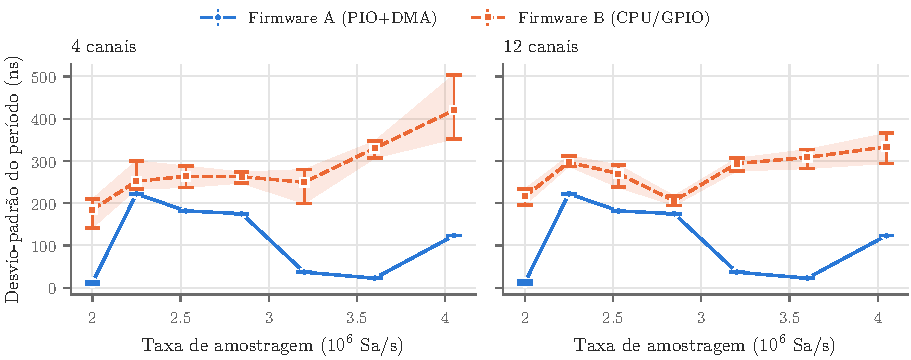
\includegraphics[width=\linewidth]{Cap04/img/m2_jitter_std.pdf}
  \fonte{Autoria própria.}
\end{figure}

O desvio-padrão do Firmware A coincide com o limite de quantização em toda
a faixa, a menos de 3,6\,ns (no máximo, um excedente de 5,9\,ns em
3,20\,MS/s), e acompanha inclusive as oscilações de $\sigma_q$ com a taxa;
as diferenças estão dentro da incerteza com que $f_{sig}$ é conhecida, o
que explica $\sigma_A$ ficar ligeiramente abaixo de $\sigma_q$ em algumas
taxas, já que $\sigma_q$ é calculado com a frequência aferida, e não com a
real.
As 30 repetições de A são praticamente idênticas, de modo que, nas figuras,
o intervalo entre o mínimo e o máximo de A fica menor que o próprio
marcador. O Firmware B fica acima de $\sigma_q$ em todas as condições, com
excedente de 106 a 400\,ns, o equivalente a 16 a 60 ciclos de \ac{CPU} a
150\,MHz, e com variação visível entre repetições. O valor pico a pico do
período separa ainda mais os dois: de 0,25 a 1,0\,\textmu s em A e de 6,3 a
13,3\,\textmu s em B, isto é, B registra intervalos entre bordas que
chegam a quase dois períodos do sinal.

A contagem de períodos (Figura~\ref{fig:m2-perdidos}) repete o padrão da
M1. Em A, a diferença para a referência fica entre $-2$ e 0, apenas o corte
da janela. Em B, a captura contém em geral \emph{mais} períodos que a
referência, até 42 a mais em 4,05\,MS/s com 4 canais (0,21\,\% da janela).

\begin{figure}[htbp]
  \centering
  \caption{M2: períodos ausentes em relação à referência.}
  \label{fig:m2-perdidos}
  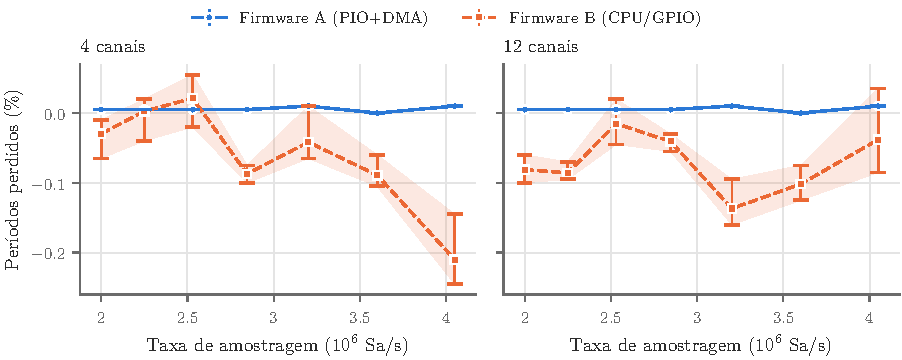
\includegraphics[width=\linewidth]{Cap04/img/m2_periodos_perdidos.pdf}
  \fonte{Autoria própria.}
  \nota{em percentual da janela; valores negativos indicam períodos a mais (sinal oposto ao de $\Delta n$ na Tabela~\ref{tab:m2-jitter}).}
\end{figure}

A comparação estatística cobre as 14 condições (sete taxas $\times$ duas
contagens de canais) e três medidas: o desvio-padrão do período, seu
valor pico a pico e a diferença na contagem de períodos
(Tabela~\ref{tab:m2-estat}). Nas duas primeiras, a separação é completa
em todas as condições ($r = +1{,}00$;
$p_{\mathrm{Holm}} \le 1{,}6 \times 10^{-10}$), com B acima de A por 20
a 311\,ns no desvio-padrão e por 5,3 a 13,1\,\textmu s no pico a pico.
Na contagem de períodos, B conta mais que A em 12 das 14 condições; a
diferença não é significativa em 2,25\,MS/s com 4 canais e se inverte
em 2,53\,MS/s com 4 canais, em até 6,5 períodos.

\begin{table}[H]
  \centering
  \caption{M2: comparação estatística das medidas de período (B $-$ A).}
  \label{tab:m2-estat}
  \resizebox{\linewidth}{!}{%
  \begin{tabular}{@{}rrrrrrr@{}}
    \toprule
    & & \multicolumn{2}{c}{\textbf{IC 95\,\% da diferença}} &
    \multicolumn{3}{c}{\textbf{Contagem de períodos} $\boldsymbol{\Delta n}$} \\
    \cmidrule(lr){3-4}\cmidrule(l){5-7}
    \textbf{Canais} & \textbf{Taxa (MS/s)} & $\boldsymbol{\sigma}$ \textbf{(ns)} &
    \textbf{pico a pico (\textmu s)} & $\boldsymbol{r}$ &
    $\boldsymbol{p_{\mathrm{Holm}}}$ & \textbf{IC 95\,\%} \\
    \midrule
    4 & 2{,}00 & $[166{,}4; 177{,}0]$ & $[10{,}2; 11{,}5]$ & $+1{,}00$ & $1{,}3 \times 10^{-11}$ & $[5{,}5; 7{,}5]$ \\
    4 & 2{,}25 & $[20{,}3; 34{,}3]$ & $[10{,}2; 10{,}7]$ & $+0{,}03$ & $8{,}1 \times 10^{-1}$ & $[-1{,}0; 1{,}0]$ \\
    4 & 2{,}53 & $[74{,}0; 90{,}1]$ & $[11{,}1; 11{,}5]$ & $-0{,}50$ & $7{,}0 \times 10^{-4}$ & $[-6{,}5; -1{,}0]$ \\
    4 & 2{,}85 & $[85{,}8; 89{,}8]$ & $[10{,}2; 10{,}9]$ & $+1{,}00$ & $1{,}3 \times 10^{-11}$ & $[18{,}0; 19{,}0]$ \\
    4 & 3{,}20 & $[208{,}3; 219{,}0]$ & $[10{,}9; 11{,}9]$ & $+0{,}97$ & $2{,}2 \times 10^{-11}$ & $[9{,}0; 12{,}0]$ \\
    4 & 3{,}60 & $[304{,}6; 310{,}8]$ & $[11{,}7; 11{,}9]$ & $+1{,}00$ & $1{,}3 \times 10^{-11}$ & $[17{,}0; 19{,}0]$ \\
    4 & 4{,}05 & $[281{,}8; 308{,}7]$ & $[11{,}4; 12{,}0]$ & $+1{,}00$ & $1{,}3 \times 10^{-11}$ & $[42{,}0; 47{,}0]$ \\
    \midrule
    12 & 2{,}00 & $[200{,}6; 210{,}2]$ & $[10{,}0; 11{,}0]$ & $+1{,}00$ & $1{,}3 \times 10^{-11}$ & $[17{,}0; 18{,}0]$ \\
    12 & 2{,}25 & $[70{,}9; 76{,}8]$ & $[10{,}2; 11{,}3]$ & $+1{,}00$ & $1{,}3 \times 10^{-11}$ & $[18{,}0; 19{,}0]$ \\
    12 & 2{,}53 & $[82{,}8; 94{,}6]$ & $[11{,}1; 11{,}5]$ & $+0{,}87$ & $2{,}2 \times 10^{-9}$ & $[3{,}0; 5{,}5]$ \\
    12 & 2{,}85 & $[28{,}1; 33{,}0]$ & $[5{,}3; 6{,}7]$ & $+1{,}00$ & $1{,}3 \times 10^{-11}$ & $[9{,}0; 10{,}0]$ \\
    12 & 3{,}20 & $[252{,}3; 262{,}8]$ & $[11{,}2; 11{,}6]$ & $+1{,}00$ & $1{,}3 \times 10^{-11}$ & $[28{,}0; 31{,}5]$ \\
    12 & 3{,}60 & $[281{,}8; 292{,}3]$ & $[12{,}5; 13{,}1]$ & $+1{,}00$ & $1{,}3 \times 10^{-11}$ & $[19{,}0; 22{,}0]$ \\
    12 & 4{,}05 & $[200{,}9; 220{,}8]$ & $[12{,}3; 12{,}8]$ & $+0{,}93$ & $1{,}3 \times 10^{-10}$ & $[8{,}0; 12{,}5]$ \\
    \bottomrule
  \end{tabular}}
  \fonte{Autoria própria.}
  \nota{$n = 30$ repetições por firmware; IC 95\,\% da diferença de medianas (B $-$ A) por \emph{bootstrap}. Em $\sigma$ e no pico a pico, $r = +1{,}00$ e $p_{\mathrm{Holm}} \le 1{,}6 \times 10^{-10}$ em todas as condições.}
\end{table}

\subsection{Discussão}

O resultado confirma o esperado (Seção~\ref{sec:determinismo}): a
amostragem pela \ac{CPU} introduz uma instabilidade de período que o
\ac{PIO} não apresenta. No Firmware A, o instante de cada amostra é
fixado pelo divisor de clock da máquina de estados e não depende
de software; o desvio observado é exatamente o de quantização, e a
medida é repetível entre capturas. No Firmware B, o laço usa prazos
absolutos no contador \ac{DWT} e ainda assim acumula dezenas de ciclos de
\emph{jitter}, porque o custo de cada iteração varia com o caminho
tomado (armazenamento, troca de \emph{buffer}, verificação de parada),
com as interrupções atendidas durante o laço, entre elas as da pilha
\ac{USB}, e com as esperas da execução a partir da flash (\acs{XIP}) e
da arbitragem de barramento.

Esse \emph{jitter} de ciclo a ciclo, porém, não explica o pico a pico de
B nem os períodos a mais: ambos apontam o mecanismo já identificado na
M1, o laço interrompido e retomado sem que o fluxo sinalize a pausa.
Acumuladas ao longo da janela, essas pausas fazem as amostras entregues
cobrirem mais que 0,2\,s, daí os períodos a mais; uma pausa que cobre um
pulso inteiro funde dois períodos em um, daí os intervalos de quase dois
períodos. A variação dessas pausas entre repetições é o que produz a
dispersão de B nas figuras, ausente em A.

\section{M3: Captura contínua e perda de amostras}\label{sec:res-m3}

\subsection{Resultado}

O ensaio aplicou a onda de 100\,kHz ao canal D3 e manteve a captura
contínua por 60\,s em cada uma das 30 repetições, com taxas a partir de
1,09\,MS/s (abaixo dela, o período tem menos de oito amostras e a detecção
de lacunas perde sensibilidade). A perda é medida de duas formas: pela
fração de amostras entregues em relação às solicitadas no tempo de captura
($f_s \times 60$\,s) e pelo número de lacunas, detectadas quando o
intervalo entre bordas se desvia do período nominal. A varredura de cada
contagem de canais para na primeira taxa em que todas as repetições
abortam ou que o firmware recusa.

O Firmware A sustentou a captura contínua em todas as 30 repetições até
3,54\,MS/s, com 4 e com 12 canais, entregando 100\,\% das amostras e sem
nenhuma lacuna (Tabela~\ref{tab:m3-resumo} e
Figuras~\ref{fig:m3-entregues} e~\ref{fig:m3-lacunas}). Em 5,24\,MS/s,
todas as repetições abortaram logo na partida, com a marca \texttt{!!!},
depois de entregar um ou dois \emph{buffers} de 1\,024 amostras
(Figura~\ref{fig:m3-abortadas}). O Firmware B recusa essa taxa na
configuração, por estar acima do teto do seu laço de amostragem, e não
abortou nenhuma captura nas taxas aceitas; em todas elas, porém, entregou
bem menos amostras do que o solicitado: de 75,7\,\% em 1,09\,MS/s a
57,3\,\% em 3,54\,MS/s, perda que cresce com a taxa e praticamente não
depende da contagem de canais.

\begin{table}[H]
  \centering
  \caption{M3: amostras entregues e lacunas em captura contínua de 60\,s.}
  \label{tab:m3-resumo}
  \begin{tabular}{@{}rrrrrrr@{}}
    \toprule
    & & \multicolumn{2}{c}{\textbf{Firmware A}} &
    \multicolumn{3}{c}{\textbf{Firmware B}} \\
    \cmidrule(lr){3-4}\cmidrule(l){5-7}
    \textbf{Canais} & \textbf{Taxa} & \textbf{Entregue} & \textbf{Lacunas} &
    \textbf{Entregue} & \textbf{Lacunas} & \textbf{Taxa efetiva} \\
    & (MS/s) & (\%) & & (\%) & & (MS/s) \\
    \midrule
    4  & 1,09 & 100,0 & 0 & 75,7 &  1\,774 & 0,83 \\
    4  & 1,62 & 100,0 & 0 & 71,2 & 10\,470 & 1,15 \\
    4  & 2,39 & 100,0 & 0 & 65,5 & 15\,398 & 1,57 \\
    4  & 3,54 & 100,0 & 0 & 58,5 & 63\,564 & 2,07 \\
    12 & 1,09 & 100,0 & 0 & 73,8 &  4\,789 & 0,81 \\
    12 & 1,62 & 100,0 & 0 & 69,5 &  8\,540 & 1,13 \\
    12 & 2,39 & 100,0 & 0 & 64,0 & 14\,882 & 1,53 \\
    12 & 3,54 & 100,0 & 0 & 57,3 & 69\,933 & 2,03 \\
    \bottomrule
  \end{tabular}
  \fonte{Autoria própria.}
  \nota{medianas de 30 repetições; taxa efetiva = amostras entregues / duração da captura.}
\end{table}

\begin{figure}[htbp]
  \centering
  \caption{M3: amostras entregues por taxa de amostragem.}
  \label{fig:m3-entregues}
  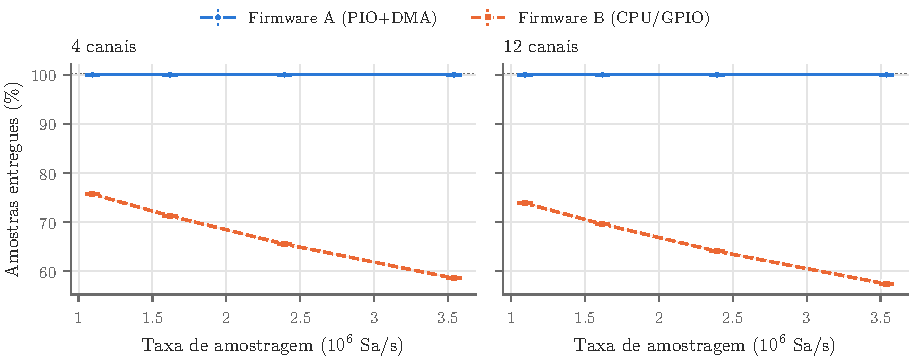
\includegraphics[width=\linewidth]{Cap04/img/m3_entregues.pdf}
  \fonte{Autoria própria.}
  \nota{em percentual das solicitadas; apenas condições sem aborto.}
\end{figure}

\begin{figure}[htbp]
  \centering
  \caption{M3: lacunas por minuto por taxa de amostragem.}
  \label{fig:m3-lacunas}
  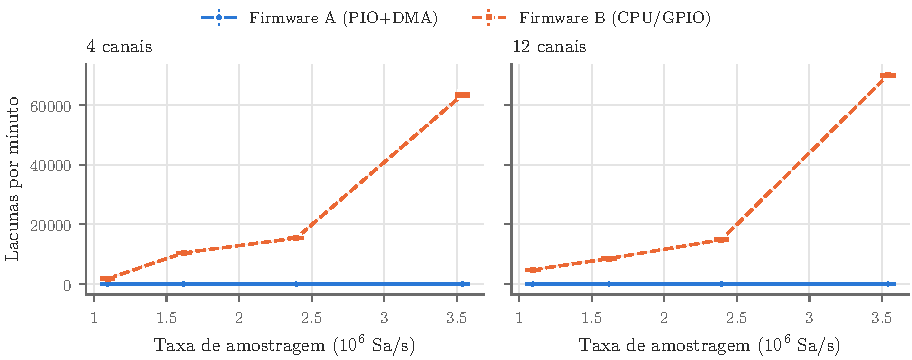
\includegraphics[width=\linewidth]{Cap04/img/m3_lacunas.pdf}
  \fonte{Autoria própria.}
  \nota{apenas condições sem aborto.}
\end{figure}

\begin{figure}[htbp]
  \centering
  \caption{M3: capturas abortadas por taxa de amostragem.}
  \label{fig:m3-abortadas}
  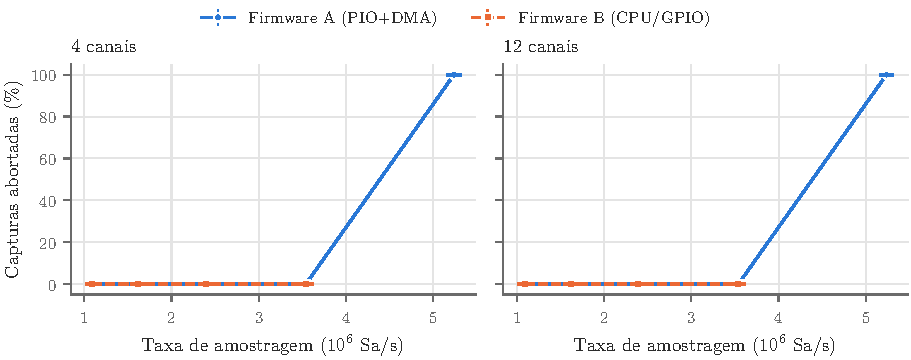
\includegraphics[width=\linewidth]{Cap04/img/m3_abortadas.pdf}
  \fonte{Autoria própria.}
\end{figure}

As duas medidas de perda de B devem ser lidas juntas. Como o sinal é
periódico, uma pausa que dure um número inteiro de períodos não altera o
intervalo entre bordas; a detecção enxerga apenas o resto da pausa em
relação ao período, e a lacuna detectada tem sempre menos de um período
(de 2 a 9 amostras, na mediana). O número de lacunas, de 1\,774 a 69\,933
por captura, é portanto um limite inferior do número de pausas, e o tamanho
das lacunas não mede a perda. A perda real é dada pela fração entregue: B
deixa de amostrar de 14 a 26\,s em cada captura de 60\,s, sem nenhuma
marca no fluxo que permita ao \emph{host} localizar esses trechos. As
lacunas de B não se concentram em nenhuma posição do bloco de $10^6$
amostras do modo contínuo (0,3\,\% delas nas primeiras 20 amostras), o que
as associa ao laço de amostragem, e não ao rearme de blocos.

Para separar o limite do barramento do limite do firmware, mediu-se
também a vazão \ac{USB} em captura contínua com sinal pouco compressível
(Figura~\ref{fig:usb-vazao}). O Firmware B satura o barramento em
$\approx 0{,}86$\,MB/s, 71\,\% do teto teórico do \ac{USB} Full-Speed
(1,216\,MB/s), e nesse regime entrega apenas 15 a 42\,\% das amostras
solicitadas. O Firmware A sustenta a captura sem perda enquanto a demanda
fica abaixo de $\approx 0{,}80$\,MB/s; acima de $\approx 0{,}92$\,MB/s,
ele aborta a captura em vez de descartar amostras.

\begin{figure}[htbp]
  \centering
  \caption{Vazão USB em captura contínua.}
  \label{fig:usb-vazao}
  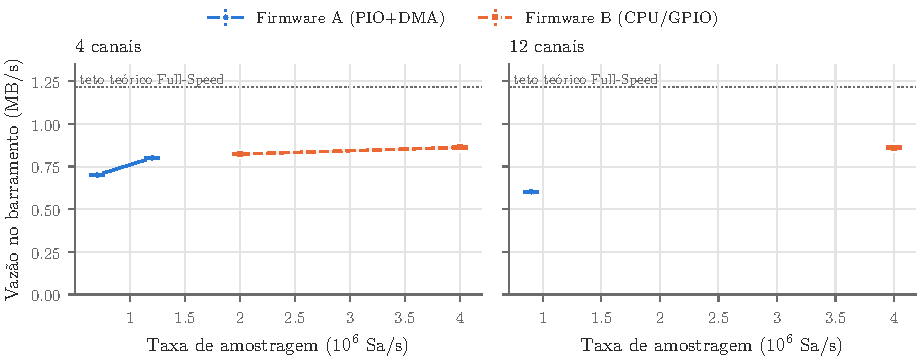
\includegraphics[width=\linewidth]{Cap04/img/usb_vazao.pdf}
  \fonte{Autoria própria.}
  \nota{apenas condições sem aborto; linha pontilhada: teto teórico do USB Full-Speed.}
\end{figure}

A comparação estatística usa as oito condições em que os dois firmwares
completaram a captura, quatro taxas $\times$ duas contagens de canais
(Tabela~\ref{tab:m3-estat}). Nas duas medidas, a separação é completa
em todas as repetições: B entrega uma fração menor das amostras
($r = -1{,}00$; $p_{\mathrm{Holm}} = 2{,}2 \times 10^{-10}$), de 24,3 a
42,7 pontos percentuais a menos, e apresenta mais lacunas
($r = +1{,}00$; $p_{\mathrm{Holm}} = 9{,}7 \times 10^{-12}$), de cerca
de 1\,800 a 70\,000 por captura. Os intervalos estreitos refletem a
baixa variação entre repetições, já que em cada condição a fração entregue
por B varia menos de 0,1 ponto percentual, isto é, a perda de B é
sistemática, e não ocasional.

\begin{table}[H]
  \centering
  \caption{M3: comparação estatística da perda de amostras (B $-$ A).}
  \label{tab:m3-estat}
  \begin{tabular}{@{}rrrr@{}}
    \toprule
    & & \multicolumn{2}{c}{\textbf{IC 95\,\% da diferença de medianas}} \\
    \cmidrule(l){3-4}
    \textbf{Canais} & \textbf{Taxa (MS/s)} &
    \textbf{Entregue (p.p.)} & \textbf{Lacunas} \\
    \midrule
    4 & 1{,}09 & $[-24{,}34; -24{,}34]$ & $[1\,748; 1\,818]$ \\
    4 & 1{,}62 & $[-28{,}79; -28{,}79]$ & $[10\,460; 10\,492]$ \\
    4 & 2{,}39 & $[-34{,}53; -34{,}53]$ & $[15\,388; 15\,410]$ \\
    4 & 3{,}54 & $[-41{,}49; -41{,}49]$ & $[63\,410; 63\,626]$ \\
    \midrule
    12 & 1{,}09 & $[-26{,}19; -26{,}19]$ & $[4\,766; 4\,822]$ \\
    12 & 1{,}62 & $[-30{,}46; -30{,}46]$ & $[8\,489; 8\,550]$ \\
    12 & 2{,}39 & $[-35{,}99; -35{,}99]$ & $[14\,869; 14\,896]$ \\
    12 & 3{,}54 & $[-42{,}68; -42{,}67]$ & $[69\,863; 70\,002]$ \\
    \bottomrule
  \end{tabular}
  \fonte{Autoria própria.}
  \nota{$n = 30$ repetições por firmware; IC por \emph{bootstrap}. Em todas as condições, $r = -1{,}00$ na fração entregue ($p_{\mathrm{Holm}} = 2{,}2 \times 10^{-10}$) e $r = +1{,}00$ nas lacunas ($p_{\mathrm{Holm}} = 9{,}7 \times 10^{-12}$).}
\end{table}

\subsection{Discussão}

O conflito entre amostrar e transmitir aparece apenas no Firmware B. Com
a onda de 100\,kHz, o fluxo compactado fica bem abaixo do teto do
\ac{USB} em toda a faixa, e A comprova isso ao entregar 100\,\% das
amostras até 3,54\,MS/s: a perda de B não vem do barramento, e sim da
disputa interna ao firmware. Em B, o laço de amostragem para enquanto um
bloco é entregue à pilha \ac{USB}, e o tempo dessas pausas cresce com a
taxa, de modo que a taxa efetiva sobe de 0,83 para apenas 2,07\,MS/s
enquanto a solicitada vai de 1,09 a 3,54\,MS/s. Em A, o \ac{DMA} continua amostrando
enquanto a \ac{CPU} transmite, e a fila de dois \emph{buffers} absorve a
variação do envio. A diferença qualitativa repete a da M1: A entrega um
fluxo sem perda dentro da faixa sustentada e aborta sinalizando fora
dela, pela mesma razão discutida na Seção~\ref{sec:res-m1} (a partida da
transferência \ac{USB} atrasa o consumo dos \emph{buffers}, e dois
\emph{buffers} cobrem menos de meio milissegundo a 5,24\,MS/s); B nunca
sinaliza e entrega, em toda a faixa, um fluxo que aparenta ser contínuo
mas em que um quarto a quase metade do tempo não foi amostrado.

Cabe registrar, como na M1, que a versão inicial do Firmware A rearmava
o \ac{PIO} e o \ac{DMA} a cada bloco de $10^6$ amostras do modo contínuo,
deixando cerca de uma lacuna silenciosa de 2,7 a 3,4\,\textmu s por
bloco, com 88,6\,\% delas nas primeiras 20 amostras. A correção passou a
armar o \ac{DMA} encadeado uma única vez por captura, e os resultados
desta seção referem-se à versão corrigida, que não apresentou nenhuma
lacuna em 240 capturas de 60\,s.

\section{M4: Ocupação de CPU}\label{sec:res-m4}

\subsection{Resultado}

A Figura~\ref{fig:m4-ocupacao} mostra a fração de ciclos em que a \ac{CPU}
esteve ocupada durante a captura, medida pelo contador \ac{DWT}, com a onda de
1\,MHz aplicada aos canais. A Tabela~\ref{tab:m4-ocupacao} traz valores
selecionados.

\begin{figure}[htbp]
  \centering
  \caption{M4: ocupação da CPU por taxa de amostragem.}
  \label{fig:m4-ocupacao}
  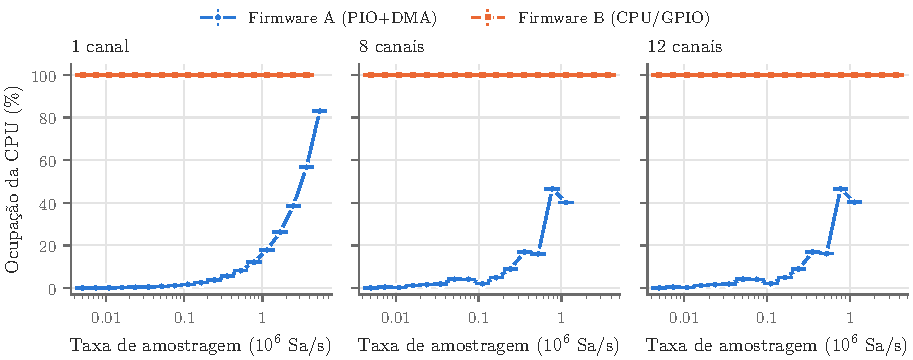
\includegraphics[width=\linewidth]{Cap04/img/m4_ocupacao.pdf}
  \fonte{Autoria própria.}
\end{figure}

\begin{table}[H]
  \centering
  \caption{M4: ocupação da CPU.}
  \label{tab:m4-ocupacao}
  \begin{tabular}{@{}rrrrr@{}}
    \toprule
    \textbf{Taxa (kS/s)} & \textbf{A, 1 canal} & \textbf{A, 8 canais} &
    \textbf{A, 12 canais} & \textbf{B (1, 8, 12 canais)} \\
    \midrule
    5,0      &  0,08 &  0,08 &  0,08 & 100,0 \\
    111,4    &  1,75 &  2,10 &  2,11 & 100,0 \\
    525,5    &  8,23 & 16,12 & 16,18 & 100,0 \\
    1\,141,7 & 17,84 & 40,16 & 40,26 & 100,0 \\
    3\,655,6 & 56,60 & ---   & ---   & 100,0 \\
    5\,388,0 & 82,95 & ---   & ---   & ---   \\
    \bottomrule
  \end{tabular}
  \fonte{Autoria própria.}
  \nota{em \%; medianas de 30 repetições.}
\end{table}

No Firmware A, a ocupação parte de 0,08\,\% e cresce com a taxa: 17,8\,\%
em 1,14\,MS/s com um canal e 83,0\,\% em 5,39\,MS/s, a maior taxa que
completou a captura. Com 8 e 12 canais, a ocupação é maior, até 46,6\,\%, e
as capturas abortam a partir de 1,68\,MS/s. No Firmware B, a ocupação é de
100\,\% em todas as condições (mínimo de 99,995\,\%), e as taxas acima de
$\approx 4{,}05$\,MS/s são recusadas pelo próprio firmware.

Esses limites não são comparáveis aos da M1, porque as condições diferem:
a M4 usa capturas curtas de quantidade fixa, com 65\,536 amostras, e onda de
1\,MHz, enquanto a M1 em 5,39\,MS/s, por exceder o limite de $10^6$
amostras, usou o modo contínuo (Seção~\ref{sec:metricas}). A causa exata
dessa diferença não foi isolada nos ensaios. Além disso, a ocupação é medida
de forma diferente nos dois firmwares: em A, conta-se como ocupado apenas o
tempo de codificação e transmissão, e não a espera pelo \ac{DMA}; em B, a captura
inteira. Os valores da M4 medem, portanto, o custo de processamento por
amostra, e não a taxa sustentada, que é dada pela M1 e pela M3.

Nas 48 condições medidas pelos dois firmwares, a separação é completa
($r = +1{,}00$, B maior em todas as repetições;
$p_{\mathrm{Holm}} \le 1{,}7 \times 10^{-10}$). Como a ocupação de B é
sempre 100\,\%, a diferença de medianas é apenas o complemento da
ocupação de A: vai de 99,9 pontos percentuais em 5\,kS/s a 43,4 pontos
em 3,66\,MS/s com um canal, e os \ac{IC}~95\,\% têm largura menor que
0,03 ponto percentual em todas as condições.

\subsection{Discussão}

A \ac{CPU} do Firmware B está, por construção, inteiramente dedicada ao
laço de amostragem: mesmo em 5\,kS/s, ela espera ativamente o prazo de
cada amostra. No Firmware A, a ocupação a baixas taxas confirma que a
\ac{CPU} fica fora do caminho de dados, mas, como previsto
(Seção~\ref{sec:metricas}), ela cresce proporcionalmente à taxa porque a
\ac{CPU} ainda percorre cada amostra para a codificação \ac{RLE}, a cerca
de 23 ciclos por amostra. É esse custo, e não a amostragem, que limita A
em taxas altas e com mais canais, quando a transição mais frequente
entre valores torna o \ac{RLE} mais caro. A arquitetura \ac{PIO}+\ac{DMA} retira a \ac{CPU} da
\emph{amostragem}, mas não do \emph{processamento} do fluxo; mover a
compactação para o \ac{PIO} ou para o segundo núcleo seria o passo seguinte para
aproximar A do ideal.

\section{Síntese e discussão}\label{sec:res-sintese}

O Quadro~\ref{qua:sintese} reúne o resultado das quatro métricas. Em todas
elas, a diferença entre os firmwares é estatisticamente significativa nas
condições em que se espera diferença, e o tamanho de efeito é, na
maioria das condições, o máximo possível ($|r| = 1$): todas as repetições
de um firmware ficam de um mesmo lado de todas as repetições do outro.

\begin{quadro}[H]
  \centering
  \caption{Síntese dos resultados.}
  \label{qua:sintese}
  \begin{tabularx}{\linewidth}{|l|>{\raggedright\arraybackslash}X|>{\raggedright\arraybackslash}X|}
    \hline
    \textbf{Métrica} & \textbf{Firmware A (\acs{PIO}+\acs{DMA})} & \textbf{Firmware B (\acs{GPIO}+\acs{CPU})} \\ \hline
    M1 & 3,66\,MS/s, contagem exata; acima disso, aborto sinalizado &
         2,48\,MS/s pelo critério de 0,1\,\% (774,6\,kS/s pelo de $\pm 2$
         bordas); bordas a mais sem sinalização \\ \hline
    M2 & $\sigma$ igual ao limite de quantização ($\le 3{,}6$\,ns de
         diferença), repetível entre capturas &
         106 a 400\,ns acima da quantização; pico a pico de até
         13\,\textmu s; até 42 períodos a mais \\ \hline
    M3 & 100\,\% das amostras e nenhuma lacuna até 3,54\,MS/s; aborto
         sinalizado em 5,24\,MS/s &
         57 a 76\,\% das amostras, sem sinalização, já a partir de
         1,09\,MS/s \\ \hline
    M4 & 0,08\,\% a 83\,\% de ocupação, proporcional à taxa (custo do \acs{RLE}) &
         100\,\% de ocupação em qualquer taxa \\ \hline
  \end{tabularx}
  \fonte{Autoria própria.}
  \nota{sinal de 100\,kHz em M1--M3 e de 1\,MHz em M4.}
\end{quadro}

\paragraph{Confronto com o esperado.} Dois comportamentos previstos na
fundamentação (Capítulo~\ref{cap:fundamentacao}) foram confirmados, o
primeiro por um mecanismo diferente do previsto (Seção~\ref{sec:res-m1}): a
arquitetura \ac{PIO}+\ac{DMA} sustenta uma taxa cerca de 1,5 vez maior (4,7 vezes
pelo critério estrito de $\pm 2$ bordas) e amostra com período fixado pelo
\emph{hardware}, sem \emph{jitter} além da quantização. O conflito entre
amostrar e transmitir apareceu apenas na arquitetura \ac{GPIO}+\ac{CPU}: com o mesmo sinal e o mesmo protocolo, A entregou o
fluxo completo enquanto B deixou de amostrar um quarto a quase metade do
tempo, o que mostra que a perda não vem do barramento, e sim de a \ac{CPU} de B
dividir o tempo entre as duas tarefas. Quanto à ocupação de \ac{CPU}, B a
ocupa por inteiro, como previsto, mas a ocupação de A só é
próxima de zero em taxas baixas, porque a codificação \ac{RLE} ainda passa por
cada amostra na \ac{CPU}.

\paragraph{Diferença qualitativa.} Mais do que os números, os dois
firmwares diferem no custo de detectar a própria falha. Em A, a condição de
falha é um evento de hardware: quando a fila de \emph{buffers} transborda, o
\ac{DMA} expõe esse estado à \ac{CPU} fora do caminho crítico da amostragem, e
o firmware converte o evento no aborto sinalizado pela marca \texttt{!!!} do
protocolo. Em B, a condição de falha é a perda de um prazo dentro do próprio
laço: a amostragem para enquanto os dados são transmitidos e, nas versões aqui
medidas, o fluxo entregue ao \emph{host} não marca essas pausas. O resultado é
uma captura que parece válida, mas cuja escala de tempo não corresponde à real,
o que se manifesta como bordas e períodos a mais (M1 e M2) ou como amostras
ausentes (M3). Para um analisador lógico, essa é a falha mais grave, porque o
usuário não tem como distingui-la de um comportamento real do circuito medido.

Cabe distinguir, porém, o que decorre da arquitetura do que decorre desta
implementação. A arquitetura impõe a \emph{existência} das pausas em B, já que
o mesmo núcleo amostra e transmite, e torna a falha de A observável sem custo
sobre a temporização da captura. A \emph{sinalização} da falha, ao contrário, é
decisão de projeto: o laço de B mantém prazos absolutos no contador \ac{DWT}
(Seção~\ref{sec:firmware-b}) e dispõe, portanto, da informação necessária para
contar os prazos perdidos e emitir um marcador de lacuna no fluxo, o que não
foi implementado nas versões aqui medidas. Que a distinção não é acadêmica
mostra-o a própria bancada: a primeira versão do Firmware A rearmava o \ac{PIO}
e o \ac{DMA} sem sinalizar a lacuna resultante e falhava em silêncio pelo mesmo
mecanismo, até receber a correção descrita na
Seção~\ref{sec:bancada-instrumentos}. O critério transferível a outras
plataformas é, assim, o custo de detectar a falha, nulo sobre o caminho
crítico quando o amostrador é um periférico independente e pago em ciclos do
laço quando o amostrador é a própria \ac{CPU}, e não a presença ou a
ausência de sinalização em um firmware específico.

O custo do laço de B ($C_{iter} = 35$ ciclos, teto de 4,29\,MS/s pela
Equação~\ref{eq:fsmax}) não explica o resultado: B falha bem abaixo desse
teto, por causa das pausas, e não por falta de ciclos.

\paragraph{Quando GPIO+CPU basta e quando PIO+DMA é indispensável.} Nas
condições medidas, a leitura de \ac{GPIO} pela \ac{CPU} basta para capturas com
disparo e janela fixa em taxas de até 774,6\,kS/s, em que a contagem de
bordas de B foi exata, e para aplicações que toleram centenas de
nanossegundos de incerteza no instante de cada amostra. Acima de
$\approx 1{,}1$\,MS/s em captura com disparo, e já a partir de
1,09\,MS/s, a menor taxa medida, em captura contínua, B passa a perder
tempo de amostragem sem sinalizar, e \ac{PIO}+\ac{DMA} se torna indispensável sempre
que a integridade do fluxo importa. \ac{PIO}+\ac{DMA} também é a única opção quando
a \ac{CPU} precisa ficar livre para outras tarefas durante a captura, já que B
a ocupa por completo. A arquitetura \ac{PIO}+\ac{DMA}, por sua vez, não elimina
todos os limites: o teto de A em 3,66\,MS/s vem da codificação \ac{RLE} na \ac{CPU}
e da fila de apenas dois \emph{buffers} do \ac{DMA}, e ambos podem ser
melhorados sem abandonar a arquitetura.

\paragraph{Ameaças à validade à luz dos dados.} Das ameaças previstas no
planejamento (Capítulo~\ref{cap:metodologia}), as que os dados não
descartam são tratadas como limitações do estudo
(Seção~\ref{sec:limitacoes}): o sinal único de M1--M3, que torna os tetos
dependentes da compressibilidade do fluxo; a variante de núcleo único do
Firmware B, a única medida; os \emph{buffers} de tamanhos diferentes, que
favorecem B e ainda assim o deixam atrás nas quatro métricas, mas tornam
o teto de A específico de sua fila de dois \emph{buffers}; e a bancada e
a plataforma únicas, cuja baixa dispersão entre repetições de A indica
que não introduziram variação relevante, sem eliminar vieses comuns às
duas arquiteturas.

\cleardoublepage
% % % % % % % % % % % % % % % % % % % % % % % % % % %
%\input{Cap05/Capitulo5}
%\cleardoublepage
% % % % % % % % % % % % % % % % % % % % % % % % % % %
%\input{Cap06/Capitulo6}
%\cleardoublepage
%%% % % % % % % % % % % % % % % % % % % % % % % % % % %
\chapter{Conclusão}\label{cap:conclusao}

Este trabalho avaliou experimentalmente o impacto da arquitetura de aquisição
em um analisador lógico embarcado de baixo custo, comparando, na mesma
plataforma RP2350 e com o mesmo protocolo, pilha \ac{USB} e codificação
\ac{RLE}, a amostragem por \ac{PIO} com transferência por \ac{DMA} (Firmware A)
e a leitura de \ac{GPIO} pela própria \ac{CPU} (Firmware B). A motivação era
transformar em dado experimental um argumento até então apenas teórico: o de
que a leitura por software é limitada pelo custo do laço e sujeita a
\emph{jitter} e a disputas com a comunicação, enquanto um periférico dedicado
amostra de forma determinística.

Os resultados mostram que a diferença entre as arquiteturas é maior no
\emph{modo de falhar} do que nos números. Dentro da faixa sustentada, o
Firmware A entregou um fluxo exato e repetível: contagem de bordas igual à da
referência até 3,66\,MS/s, \emph{jitter} igual ao limite de quantização e
nenhuma amostra perdida em captura contínua até 3,54\,MS/s; fora dessa faixa,
ele interrompe a captura e sinaliza o erro ao \emph{host}. O Firmware B, por
sua vez, nunca sinalizou falha, mas, a partir de $\approx 1{,}1$\,MS/s,
entregou capturas cuja escala de tempo não corresponde à real: bordas e
períodos a mais nas capturas com disparo e perda de um quarto a quase metade
das amostras em captura contínua. A causa não é o custo de cada iteração do
laço, que permitiria cerca de 4,29\,MS/s, mas as pausas do laço enquanto a
mesma \ac{CPU} transmite os dados. Em resposta ao objetivo geral
(Capítulo~\ref{cap:introducao}), a leitura de \ac{GPIO} pela \ac{CPU} em núcleo
único, com o mesmo núcleo amostrando e transmitindo, basta para capturas
curtas com disparo em taxas de até centenas de kS/s, quando
incertezas de centenas de nanossegundos no instante de amostragem são
aceitáveis; acima disso, e sempre que a captura é contínua ou a \ac{CPU}
precisa ficar livre, o par \ac{PIO} associado a \ac{DMA} é indispensável.

\section{Atendimento aos objetivos}

O objetivo geral foi atendido por meio de três frentes de trabalho:

\begin{enumerate}
  \item A segunda arquitetura de aquisição, por leitura de \ac{GPIO} pela \ac{CPU}, foi
        implementada mantendo idênticos o protocolo sigrok-pico, a pilha \ac{USB} e a
        codificação \ac{RLE}, de modo que as diferenças entre os firmwares comparados
        se limitam à arquitetura de aquisição e ao que dela decorre (disparo e tamanho
        dos \emph{buffers}) (Seções~\ref{sec:firmware-a} e~\ref{sec:firmware-b}).
  \item As quatro métricas (taxa máxima sustentada, \emph{jitter} de amostragem, perda
        de amostras em captura contínua e ocupação de \ac{CPU}) foram definidas e
        instrumentadas, incluindo a medição de ocupação pelo contador de ciclos
        \ac{DWT}, exposta ao \emph{host} por um comando dedicado do protocolo
        (Seção~\ref{sec:metricas}).
  \item A bancada foi montada com gerador de onda, analisador lógico de referência
        armado na mesma borda que o \ac{DAQ} e \emph{scripts} publicamente
        disponíveis \cite{dias2026artefatos}, que
        executaram de forma automatizada as 30 repetições de cada condição para os dois
        firmwares e a análise estatística correspondente (Seções~\ref{sec:bancada}
        e~\ref{sec:analise-estatistica}).
\end{enumerate}

\section{Contribuições}

A principal contribuição é a comparação controlada entre as duas arquiteturas
de aquisição na mesma plataforma, com o mesmo protocolo, a mesma pilha \ac{USB}
e a mesma codificação \ac{RLE}, lacuna identificada na literatura consultada,
em que as duas abordagens aparecem descritas, mas não medidas lado a lado sob
condições idênticas. Dela resulta o dado que o trabalho entrega a quem projeta
firmware de instrumentação embarcada, em especial analisadores lógicos,
osciloscópios de baixo custo e demais aquisições baseadas em microcontrolador:
a faixa de taxas em que a leitura de \ac{GPIO} por software ainda basta no
RP2350 é de até 774,6\,kS/s com contagem exata em captura com disparo e aquela
a partir da qual o periférico dedicado se torna indispensável é de $\approx
  1{,}1$\,MS/s em captura com disparo e já em 1,09\,MS/s, a menor taxa medida, em
captura contínua. A escolha da arquitetura de captura passa, assim, a poder se
apoiar em medida, e não em intuição ou na disponibilidade do periférico.

Além dos números, o trabalho mostra que o critério de escolha não deve ser
apenas a taxa máxima, mas também o custo de detectar a falha em cada
arquitetura. Quando o amostrador é um periférico independente, a condição de
falha é um evento de hardware, o transbordo da fila de \emph{buffers}, que a
\ac{CPU} observa fora do caminho crítico da amostragem, de modo que
recusar explicitamente a captura que não se consegue sustentar não custa nada
à temporização. Quando o amostrador é a própria \ac{CPU}, a condição de falha
é a perda de um prazo dentro do laço, e detectá-la consome ciclos do mesmo
laço que já é o recurso escasso. Nas versões aqui medidas, essa diferença
aparece na forma extrema: A aborta sinalizando, B degrada em silêncio,
entregando capturas que parecem válidas e cuja escala de tempo não corresponde
à real, falha mais grave em um instrumento de medição, porque o usuário não tem
como distingui-la de um comportamento real do circuito observado.

Convém, no entanto, separar arquitetura de implementação. O que a arquitetura
impõe é a existência das pausas na leitura por software, quando o mesmo núcleo
amostra e transmite, e a observabilidade da falha sem custo de temporização no
caminho por \ac{PIO} e \ac{DMA}. Já a sinalização é decisão de projeto: o laço
do Firmware B mantém prazos absolutos no contador \ac{DWT} e poderia contar os
prazos perdidos e marcar as lacunas no fluxo, o que não foi implementado. A
própria validação da bancada ilustra o ponto, pois a primeira versão do
Firmware A falhava em silêncio pelo mesmo mecanismo até ser corrigida
(Seção~\ref{sec:bancada-instrumentos}). O critério que se propõe como
transferível a outras plataformas é, portanto, o custo de detecção da falha, e
não o comportamento de um firmware específico.

O trabalho também deixa como produtos os dois firmwares, os \emph{scripts} de
medição e análise e os dados brutos, publicamente disponíveis
\cite{dias2026artefatos} para que o experimento possa ser auditado e repetido
por terceiros.

\section{Limitações e ameaças à validade}\label{sec:limitacoes}

Os resultados devem ser lidos dentro das condições em que foram obtidos. O
Quadro~\ref{qua:limitacoes} reúne as limitações do estudo e o alcance que cada
uma restringe.

\begin{quadro}[H]
  \centering
  \caption{Limitações do estudo.}
  \label{qua:limitacoes}
  \small
  \begin{tabularx}{\linewidth}{|>{\raggedright\arraybackslash}p{3.0cm}|>{\raggedright\arraybackslash}X|>{\raggedright\arraybackslash}X|}
    \hline
    \textbf{Limitação} & \textbf{O que ficou de fora}                                                                                                                                                                                                           & \textbf{Alcance do resultado} \\ \hline
    Sinal único em M1--M3
                       & Onda quadrada de 100\,kHz em um só canal; não se variou frequência nem densidade de transições
                       & Como o \ac{RLE} torna a demanda de banda dependente do sinal, sinais mais rápidos ou com mais transições reduzem os tetos dos dois firmwares, como mostrou o ensaio descartado a 1\,MHz                                                                                \\ \hline
    Apenas a variante de núcleo único do Firmware B
                       & A variante que dedica um núcleo à amostragem e outro à transmissão (Seção~\ref{sec:firmware-b})
                       & É justamente a que poderia reduzir as pausas observadas; o teto medido de B vale para a variante de núcleo único                                                                                                                                                       \\ \hline
    \emph{Buffers} de tamanhos diferentes
                       & 1\,024 amostras em A contra 8\,192 em B, sem equalização
                       & A diferença favorece B, de modo que não inverte as conclusões, mas o teto de A em M1 e M3 é específico de sua fila de dois \emph{buffers} de 1\,024 amostras                                                                                                           \\ \hline
    Bancada única
                       & Uma placa, um \emph{host} e um analisador de referência sem calibração rastreável
                       & A baixa dispersão entre repetições de A indica que a bancada não introduziu variação relevante, mas não elimina vieses comuns às duas arquiteturas                                                                                                                     \\ \hline
    Plataforma única
                       & Somente o RP2350 a 150\,MHz
                       & Os números são específicos dessa plataforma; a estrutura do resultado: \ac{CPU} dividida entre amostrar e transmitir contra um periférico que amostra sozinho, tende a se repetir em outros microcontroladores, com valores diferentes                                 \\ \hline
  \end{tabularx}
  \fonte{Autoria própria.}
\end{quadro}

Além dessas limitações, o planejamento do experimento
(Capítulo~\ref{cap:metodologia}) identificou ameaças à validade em quatro
categorias: \textbf{conclusão}, se as diferenças observadas são
estatisticamente confiáveis; \textbf{interna}, se elas se devem à arquitetura
de aquisição e não a outro fator; \textbf{construto}, se as métricas medem de
fato a propriedade pretendida; e \textbf{externa}, até onde os resultados se
generalizam. O Quadro~\ref{qua:ameacas} reúne cada ameaça e a mitigação
adotada.

\begin{quadro}[H]
  \centering
  \caption{Ameaças à validade e mitigações.}
  \label{qua:ameacas}
  \small
  \begin{tabularx}{\linewidth}{|>{\raggedright\arraybackslash}p{2.0cm}|>{\raggedright\arraybackslash}X|>{\raggedright\arraybackslash}X|}
    \hline
    \textbf{Categoria} & \textbf{Ameaça}                                                                                    & \textbf{Mitigação} \\ \hline
    Conclusão          & Poder estatístico limitado para efeitos pequenos, mesmo com $N = 30$ \cite{cohen1988}
                       & Tamanho de efeito e \acs{IC} reportados junto a cada teste                                                              \\ \cline{2-3}
                       & Múltiplos testes por métrica (taxas $\times$ canais)
                       & Correção de Holm--Bonferroni por família de métrica                                                                     \\ \hline
    Interna            & Variações do \emph{host} (escalonamento do sistema operacional, outras cargas \acs{USB})
                       & Mesmo \emph{host} dedicado, repetições e relato da dispersão                                                                   \\ \cline{2-3}
                       & Diferenças entre os firmwares além da amostragem: disparo e tamanho dos \emph{buffers}
                       & Diferenças restritas às que decorrem da arquitetura; \emph{buffers} maiores em B, o que o favorece                      \\ \cline{2-3}
                       & Referência com base de tempo sem calibração rastreável
                       & Erro do cristal (dezenas de ppm) muito abaixo das diferenças medidas                                                    \\ \cline{2-3}
                       & Esforço de depuração assimétrico: a sinalização de falha só foi implementada em A, cuja primeira versão falhava em silêncio até ser corrigida
                       & Distinção explícita entre o que decorre da arquitetura (existência das pausas, observabilidade do transbordo) e o que decorre da implementação (sinalização), tratada na Seção~\ref{sec:res-sintese} \\ \hline
    Construto          & Banda \acs{USB} dependente do sinal por causa do \acs{RLE}
                       & Mesmo sinal nos dois firmwares; 100\,kHz mantém o fluxo abaixo do teto do \acs{USB}                                     \\ \cline{2-3}
                       & Definição de ``ocupado'' diferente entre os firmwares em M4
                       & Definição explicitada (Seção~\ref{sec:metricas}) e ligada à arquitetura                                                 \\ \cline{2-3}
                       & Lacunas de duração múltipla do período não detectadas em M3
                       & Fração entregue como medida principal; lacunas como limite inferior                                                     \\ \hline
    Externa            & Um único sinal, em um único canal, em M1--M3
                       & Ensaio auxiliar com sinal pouco compressível (Seção~\ref{sec:metricas})                                                 \\ \cline{2-3}
                       & Uma placa, um \emph{host}, RP2350 a 150\,MHz e apenas a variante de núcleo único de B
                       & Generalização feita apenas de forma qualitativa                                                                         \\ \hline
  \end{tabularx}
  \fonte{Autoria própria.}
\end{quadro}

As mitigações reduzem, mas não eliminam, essas ameaças. As que permaneceram
relevantes à luz dos dados, em especial o sinal único e a variante de núcleo
único do Firmware B, são as retomadas no Quadro~\ref{qua:limitacoes} e nos
trabalhos futuros a seguir.

\section{Trabalhos futuros}\label{sec:trabalhos-futuros}

Os desdobramentos identificados organizam-se em três frentes, resumidas no
Quadro~\ref{qua:futuros}: \textbf{elevar os tetos} de cada arquitetura,
atacando as causas isoladas no Capítulo~\ref{cap:resultados}; \textbf{isolar as
  causas} que o experimento apontou mas não decompôs, em especial as fontes do
\emph{jitter} do Firmware B; e \textbf{ampliar a validade} dos resultados para
além das condições do Quadro~\ref{qua:limitacoes}.

\begin{quadro}[H]
  \centering
  \caption{Trabalhos futuros.}
  \label{qua:futuros}
  \small
  \begin{tabularx}{\linewidth}{|>{\raggedright\arraybackslash}p{2.1cm}|>{\raggedright\arraybackslash}X|>{\raggedright\arraybackslash}X|}
    \hline
    \textbf{Frente} & \textbf{Trabalho proposto}                                                                                                                                                       & \textbf{Origem e resultado esperado} \\ \hline
    Elevar os tetos
                    & Medir a variante de dois núcleos do Firmware B, com amostragem e transmissão em núcleos distintos (Seção~\ref{sec:firmware-b})
                    & As pausas do laço, e não o custo da iteração, limitam B (Seção~\ref{sec:res-m1}); separar as tarefas deve aproximar a taxa sustentada dos $\approx 4{,}29$\,MS/s do teto do laço                                        \\ \cline{2-3}
                    & Tirar a codificação \ac{RLE} da \ac{CPU} do Firmware A, por um programa \ac{PIO} ou pelo segundo núcleo, e aprofundar a fila de \emph{buffers} da \ac{DMA}, hoje limitada a dois
                    & O teto de A vem do consumo das amostras, não da amostragem (Seções~\ref{sec:res-m1} e~\ref{sec:res-m4}); ambos são melhoráveis sem trocar de arquitetura                                                                \\ \hline
    Isolar as causas
                    & Medir o \emph{jitter} do Firmware B com o laço executado da flash (\acs{XIP}) \emph{versus} da \ac{SRAM} e com interrupções habilitadas \emph{versus} desabilitadas
                    & A discussão da M2 atribui o \emph{jitter} a várias fontes somadas (Seção~\ref{sec:res-m2}); o ensaio diria o peso de cada uma                                                                                           \\ \cline{2-3}
                    & Medir externamente, por osciloscópio em modo histograma ou persistência, um pino de \emph{debug} comutado pelo laço de amostragem
                    & Verificação independente do \emph{jitter}, hoje obtido pela análise dos períodos capturados, sem depender do próprio caminho de dados sob teste                                                                         \\ \hline
    Ampliar a validade
                    & Repetir as medições com sinais de frequências e densidades de transição variadas, em vários canais simultaneamente
                    & Levanta a limitação do sinal único (Quadro~\ref{qua:limitacoes}) e separa o efeito do \ac{RLE} do efeito da arquitetura                                                                                                 \\ \cline{2-3}
                    & Avaliar a latência de disparo e a decodificação de protocolos reais nas duas arquiteturas
                    & Estende a comparação a propriedades que as quatro métricas não cobrem, mas que definem o uso prático de um analisador lógico                                                                                            \\ \hline
  \end{tabularx}
  \fonte{Autoria própria.}
\end{quadro}

Entre elas, a variante de dois núcleos do Firmware B é a mais imediata: é a
única que pode alterar a conclusão prática deste trabalho, já que ataca
exatamente o mecanismo que limita a arquitetura por software nas quatro
métricas medidas: as pausas do laço enquanto a mesma \ac{CPU} transmite os
dados.

\cleardoublepage
%%% % % % % % % % % % % % % % % % % % % % % % % % % % %
%%% % % % % % % % % % % % % % % % % % % % % % % % % % %
\markright{Referências}
%\renewcommand\bibname{Bibliography}

% % % % % % % % % % % % % % % % % % % % % % % % % % %
% Definir estilo bibliográfico  % % % % % % % % % % %
% % % % % % % % % % % % % % % % % % % % % % % % % % %

\bibliographystyle{abntex2-alf}
%%
{
	\renewcommand{\bibname}{REFER\^ENCIAS}
	\cleardoublepage
	\phantomsection
	\addcontentsline{toc}{chapter}{Referências}
	\bibliography{Ref/referencias}
}
\cleardoublepage
%%% % % % % % % % % % % % % % % % % % % % % % % % % % %
%%% % % % % % % % % % % % % % % % % % % % % % % % % % %

% Apendice vazio: reativar quando houver conteudo
%\appendix

\cleardoublepage

\end{document}
